
\documentclass[11pt]{article}
\usepackage[margin=1.1in]{geometry}
\usepackage{amsmath,amssymb,amsthm,mathtools}
\usepackage{booktabs}
\usepackage{array}
\usepackage[dvipsnames]{xcolor}
\usepackage{tikz}
\usetikzlibrary{arrows.meta,calc,shadings}
\usepackage[colorlinks=true,linkcolor=MidnightBlue,citecolor=MidnightBlue,urlcolor=MidnightBlue]{hyperref}

\newtheorem{theorem}{Theorem}[section]
\newtheorem{proposition}[theorem]{Proposition}
\newtheorem{lemma}[theorem]{Lemma}
\newtheorem{corollary}[theorem]{Corollary}
\theoremstyle{definition}
\newtheorem{definition}[theorem]{Definition}
\newtheorem{remark}[theorem]{Remark}
\newtheorem{example}[theorem]{Example}
\newtheorem{conjecture}[theorem]{Conjecture}
\newtheorem{fact}[theorem]{Fact}
\newtheorem{observation}[theorem]{Observation}
\newtheorem{premise}[theorem]{Premise}
\newtheorem{question}[theorem]{Question}

\newcommand{\Cl}{\mathrm{Cl}}
\newcommand{\R}{\mathbb{R}}
\newcommand{\C}{\mathbb{C}}
\newcommand{\T}{\mathbb{T}}
\newcommand{\Mat}{\mathrm{M}}
\newcommand{\End}{\operatorname{End}}
\newcommand{\tr}{\operatorname{tr}}
\newcommand{\id}{\mathrm{id}}
\newcommand{\ip}[2]{\langle #1, #2\rangle}
\newcommand{\br}[1]{\langle #1\rangle}
\newcommand{\Neff}{N_{\mathrm{eff}}}
\let\oldsection\section
\renewcommand{\section}{\clearpage\oldsection}   % every section starts on a new page (Leon, 2026-09-26)
\newcommand{\B}{\mathrm{B}}
\newcommand{\Sph}{\mathrm{S}}
\newcommand{\dS}{\mathrm{dS}}

\title{\bfseries Dark Matter and the Arrow of Time\\[4pt]
  \large\itshape The Dark Towers}
\author{Leon Butler\\ \normalsize\href{mailto:lbutler.math@gmail.com}{\texttt{lbutler.math@gmail.com}}\\ \normalsize ORCID: \href{https://orcid.org/0009-0006-4449-5617}{0009-0006-4449-5617}}
\date{Version 2.0, September 2026 \textperiodcentered{} Transport Papers, T14}

\begin{document}
\maketitle

\begin{abstract}
\normalsize
Transport runs in eight parallel towers, the residues of the Clifford clock. At the dimension nearest four (a flagged premise) two towers are sterile, $r = 4$ with no time and $r = 0$ with two (an imported fork): six can hold matter, five dark; the mirror is populated by indifference, the odd four by inference from the observed remainder. The residue is soldered, not algebraic, so the one metric superselects tower charge: exact stability, given the sector decomposition and the wall displacement. The mirror tower is proved a copy of whatever the Standard-Model paper derives: a second Standard Model, one visible share to half a percent, given one orientation. The orientation bit is the chirality of the pure spinor, its two halves in opposite families only at tower dimension a multiple of four, so the odd residues have no bit and asymmetric dark matter is the mirror tower's. The odd towers' symmetric relic needs a coupling rule the series lacks. One geometric rule, a common mass quantum per unit ball of each tower's space, returns the dark matter ratio as $(11\pi + 16)/(3\pi) = 5.364$ against $5.364 \pm 0.065$ observed, found by fitting, at observation level on three premises; the floor $5.255$ holds for every thickness. The mirror's share is the testable claim, already a quarter above the galactic bound on mirror matter. The same bit is argued to be the arrow of time, given a three-way classification of arrows. Tier C: nine premises and a hypothesis are attacked, refutations costed, every identity script-checked.
\end{abstract}

\medskip
\noindent\textbf{MSC 2020.} Primary 83F05, 81V25; Secondary 15A66, 81T12, 85A40.\\
\textbf{Keywords.} dark matter; hidden sectors; Clifford algebra periodicity; matter-antimatter asymmetry; arrow of time; effective number of neutrinos; self-interacting dark matter.

\newpage
\textbf{Authorship and disclosure. }The founding idea of the series is the author's: that division by zero in a Clifford algebra should be read not as a prohibition but as a transport into a higher-dimensional algebra, and that the transported division need not be accompanied by an inverse operation. The direction of investigation and the critical review of the results are likewise the author's. The mathematical development and the drafting of the text were carried out in extended collaboration with Claude Fable 5 (Anthropic), an AI system. The papers of the series are deposited in the Transport Papers community on Zenodo, \url{https://zenodo.org/communities/transport-papers}.

\newpage
\section{Introduction}\label{sec:intro}

The tower paper of this series proves that the (1,1) ascent preserves the signature residue $p - q$ modulo eight, so the transport construction runs in eight parallel towers, one per residue of the real Clifford clock \cite{ButlerT3}. Applied to the matter that gravitates and does not shine, the towers give the mirror's share of it by theorem, prove that the other four shares cannot be derived from the series as it stands, and then, by one geometric rule on three premises of its own, return the whole ratio as a closed form, $(11\pi + 16)/(3\pi) = 5.364$, found by fitting. The paper's level is Tier C: nine premises and a hypothesis, each stated before use, attacked in its own section and carried with its cost, and a falsifiability section that says how each claim would be refuted.

The chain, in outline. A residue fixes no signature, so one must be chosen for each; at the dimension nearest four (Premise P3, with the census of what other choices give) a residue has a single time when the chosen signature has exactly one timelike direction, and two residues fail, $r = 0$ with two times and $r = 4$ with none, the fixed points of the mirror map. Six towers can hold matter, this one and five dark; that they do is a theorem for the mirror (indifference along the reversal orbit) and an inference from the observed remainder for the odd four, since the framework has no other dark candidate (Observation \ref{obs:population}). The flag does not refine the sort (Witt's theorem), so the $r = 0$ exclusion rests on a two-time import alone, carried as a fork. The five are dark by superselection: the residue is an invariant of the algebra soldered to the metric, not of the algebra alone ($\Cl(1,3)$ and the sterile tower's $\Cl(0,4)$ are the same algebra, $\Mat(2, \mathbb{H})$), so no operator built from the one metric changes residue, and given the sector decomposition the towers are exactly stable, touching this one only by weight. The descent's one orientation, the flag bit, is the chirality of the pure spinor, and its two halves lie in opposite families only when the tower's dimension is a multiple of four: the odd residues cannot be oriented, the even ones can at their P3 representatives, and the asymmetric dark matter is the mirror tower's alone.

Of the five dark towers this paper derives the contribution of one, the mirror's, by theorem, and gives the other four by a rule:
\begin{gather*}
\frac{\Omega_{\mathrm{dark}}}{\Omega_{b}} \;=\; \underbrace{1}_{\text{mirror, derived, to half a percent}} \;+\; \underbrace{2 \cdot \frac{4}{3} + 2 \cdot \frac{8}{3\pi}}_{\text{four odd towers, the unit-ball rule, fitted}} \;=\; \frac{11\pi + 16}{3\pi} \;=\; 5.364,\\[6pt]
\text{against the survey's}\quad
\frac{\Omega_{c}}{\Omega_{b}} \;=\; 5.364 \pm 0.065.
\end{gather*}
The first term is a theorem (Theorem \ref{thm:share}). Everything the Standard-Model paper builds this tower's content from is invariant under the signature reversal that carries $(1,3)$ to the mirror's $(3,1)$, so the mirror tower is a second Standard Model, a massless mirror photon and mirror neutrinos included; with P2 its share is one to half a percent (the half percent is the mean mass per baryon of a helium mirror), at any mirror temperature, because the stored asymmetry is a charge of the descent and not a thermal number. The share is exact and fragile (one flavour's difference at the ceiling would move it by a factor between $4.89$ and $21.4$), and it is already at the edge of the record's bound on dissipative dark matter.

The second term is not derived: the odd towers carry no asymmetry (Theorem \ref{thm:paritybit}), and a symmetric relic's density needs a coupling rule the series does not supply (Proposition \ref{prop:norule}). What the paper offers instead is the unit-ball rule of Section \ref{sec:rule}: every populated tower holds one quantum of a common mass per unit ball of its own space, in one common unit, and its matter enters the one metric per unit of our volume through one cell radius of each direction its neighbour lacks. A tower's share is then the ratio of unit-ball volumes $V_{3}/V_{D}$: $\tfrac{4}{3}$ for each three-dimensional tower, $\tfrac{8}{3\pi}$ for each five-dimensional one.

The rule rests on three premises the series does not supply, and it was found by fitting. Its one length, the thickness of the direction we cannot see, is a premise; a contact mechanism returns its value from four clauses on how cells meet a world, each with an alternative the observation excludes, and that mechanism explains the value without deriving it. With the thickness left as a parameter the total has a floor at $5.255$, the family's one prediction independent of it, and meets the observed value at one unit and at $\tfrac{\pi}{2}$ units, the chord and the arc of a quarter turn of the nested spheres. The series' one length, the de Sitter radius, makes the spheres physical, but its reductions give totals of $5$, $5.67$ or $4.33$; the inverse-square law shows the thickness is not a gravitational quantity; and the three-dimensional towers' sheets, which momentum conservation displaces with the matter, respond to gravity in full, so that a Boltzmann computation returns the standard model's linear spectra for the rule's composition. All of this is at observation level with each cost stated (Table \ref{tab:costs}), and it changes nothing derived.

The rest of the paper: a projection lemma makes every tower's content dilute as this tower's does; the radiation audit closes the three-dimensional towers by theorem plus Polyakov and leaves the mirror (whose cost is a seeded temperature below $0.448$ of ours) and the five-dimensional towers as open channels; the orientation is shown to be the arrow itself (the seventeenth refutation); infall through this tower's horizons is routed through parallel boundary mode spaces at one wall; and the rung scale is valued conditionally at $3.5 \times 10^{11}$ to $6 \times 10^{14}$ GeV. The exposures are five species, gravity-only coupling, composite self-interaction in the three-dimensional towers, which the galaxy-cluster simulations exclude unless their matter is collisionless, dissipative mirror matter against the dark-disk and collisional-fraction bounds, dark neutron-star mergers with our tidal deformability and no counterpart, permanent direct-detection nulls, and a dimmed final burst for evaporating black holes; Section \ref{sec:premises} collects every prediction in one table.

\subsection*{Prior art}

The mod-8 periodicity of the real Clifford algebras is Bott's and Cartan's, imported through the taxonomy and tower papers \cite{ButlerT1, ButlerT3}. Hidden-sector and mirror-matter dark matter has a long literature \cite{FootMirror2004}; asymmetric dark matter, with its signature GeV-scale mass from a shared asymmetry, likewise \cite{Zurek2014}; the framework differs in deriving the sector count, the stability and the asymmetry's confinement to the oriented towers from one structure rather than positing them, and its exposure is the mirror share, mirror matter in Foot's sense. Confinement of compact three-dimensional electrodynamics is Polyakov's \cite{Polyakov1977}. The observational inputs (the $\Omega_{c}/\Omega_{b}$ ratio, the $\Neff$ cap, cluster-merger bounds on self-interaction) are the survey record's \cite{Planck2018, Clowe2006}, refreshed at submission. What this paper claims as new is listed under its contributions.

\subsection*{Contribution}

(1) Towers as residues, the single-clock filter under the nearest-dimension premise with its census, the Witt-theorem observation that the flag cannot refine the count, the spinor type by residue, and the residue as a soldered invariant (Section \ref{sec:towers}). (2) Dark and exactly stable by superselection, given the sector decomposition; the flag bit at tower dimension $0 \bmod 4$ and which towers can carry the arrow; the mode counts; the mirror tower a copy of this one, its share of one to half a percent the one derived share of the ratio; the asymmetry as a charge (Sections \ref{sec:towers}, \ref{sec:count}). (3) The asymmetry as the arrow counted, and the orientation as the arrow, both refutations carried as results (Section \ref{sec:arrow}). (4) The projection lemma, the radiation audit with its two open channels, the infall computation, and the valued ceiling (Section \ref{sec:audits}). (5) The unit-ball rule for the remainder: the odd towers' shares as ratios of unit-ball volumes, the closed form $(11\pi + 16)/(3\pi)$, a contact mechanism that returns its one length on four costed clauses, the one-parameter family as sensitivity with the floor it predicts, the de Sitter reading that fixes the unit but not the thickness, and the rule's consistency with locality, the inverse-square law and, by a recorded Boltzmann computation, the linear CMB and matter power spectra, all at observation level with the costs stated (Section \ref{sec:rule}). (6) The premises attacked, every claim stated with its cost, and every prediction collected with its level and test (Section \ref{sec:premises}). (7) Machine verification of every computational identity in exact arithmetic, including the census that could have falsified the sort \cite{ButlerVerifyT14}.

\section{Setting, premises, and imports}\label{sec:setting}

Five premises carry the derived content: P1 and P2 are the series' own, P3 and P4 this paper's, P5 decides the infall computation. Each is attacked and costed in Section \ref{sec:premises}; the unit-ball rule's premises are stated in Section \ref{sec:rule}.

\begin{premise}[P1: the single frozen point]\label{prem:single}
The descent was one event freezing one $I$ and making one orientation choice: all towers couple to one metric and are oriented, where they can be, by the one Witt flag of that event (Definition \ref{def:flag}). The orientation clause is used only on the reversal orbit, where the identification of the flag across the two towers is canonical. \emph{Support:} \cite[Thm.~4.7]{ButlerT6}, \cite[Obs.~7.4]{ButlerT12}; the orientation clause is this paper's. Structural premise.
\end{premise}

\begin{premise}[P2: indifference]\label{prem:indiff}
The descent cannot instantiate uncaused distinctions \cite[Principle~5.4]{ButlerT8}, \cite[\S2]{ButlerT13}: it equates along symmetry orbits and never equates inequivalent components. The residues are inequivalent as soldered algebras (Theorem \ref{thm:soldered}) except along the reversal $r \mapsto -r$ (exchanging $2 \leftrightarrow 6$, $1 \leftrightarrow 7$, $3 \leftrightarrow 5$, fixing $0$, $4$), so P2 equates along that orbit only; which of $2$, $6$ is visible is declared indexical. Structural premise.
\end{premise}

\begin{premise}[P3: nearest-dimension representatives]\label{prem:window}
Each tower is represented at the dimension nearest four; where two are equally near (the odd residues, three and five), the lower one with a single time, else the higher. \emph{Support:} P1's one metric read as minimality. Structural premise; Proposition \ref{prop:residues}(iii) records the other windows.
\end{premise}

\begin{premise}[P4: democracy of the asymmetry over the oriented towers]\label{prem:democracy}
The flag acts on every oriented tower's modes at one strength, $\epsilon_{r} = \epsilon$ per mode (not equal mode counts or masses). A theorem for the mirror (Theorem \ref{thm:mirror}(v)), void for the odd residues (Corollary \ref{cor:whocarries}), a premise only on the fork $r = 0$.
\end{premise}

\begin{fact}[imported: the eight towers and the mod-8 clock]\label{fact:towers}
The (1,1) ascent preserves $p - q$ and $\Cl(p+k, q+k) \cong \Mat(2^{k}, \Cl(p,q))$ (Bott), so the eight residues label eight parallel towers. \emph{Provenance:} \cite[Thms.~3.2, 3.6, Rem.~3.7]{ButlerT3}, \cite[\S7]{ButlerT1}.
\end{fact}

\begin{fact}[imported: gravity-only coupling]\label{fact:acoustic}
Within the s-wave current algebra, matter that gravitates on this metric and carries no shared gauge charge does nothing else observable. \emph{Provenance:} the acoustic no-go \cite[\S5]{ButlerT10}, at its mixed level: the sphere step conditional on the entropy paper's Indifference premise, the thermal state on the singularity paper's premise (Q).
\end{fact}

\begin{fact}[imported: the frozen norm and the registered $w = -1$]\label{fact:frozen}
The frozen point's norm is covariantly constant, $w = -1$, a registered stance \cite[Prop.~4.2]{ButlerT10}, proved on the Einstein region and conditional off it. Not used in any proof here.
\end{fact}

\begin{fact}[imported: the trichotomy and the descent's data]\label{fact:trichotomy}
\cite[Prop.~7.6]{ButlerT12}: (1) \emph{kinematic}: the rescaling covariance fixes every discrete invariant (proved), and no construction from the conformal class and pair structure alone fixes $N$ (observation level); (2) \emph{non-dynamical}: the frozen action is $N$-insensitive (imported); (3) \emph{conditional}: if kinematic, dynamical and initial-data are exhaustive (not proved), $N$ is initial data, located at the origin at observation level; (4) \emph{parameter of the laws} (imported): the three are not exhaustive, since under the action as written $N$ is constant on every solution and varies across $\Lambda$, a parameter of the laws \cite[Prop.~5.8]{ButlerT10}, so that (3) holds only if the frozen point's norm is promoted to the value of a Lagrange-multiplier field, a decision that paper records open. Wherever this paper calls a datum initial data of the descent ($\epsilon$, Proposition \ref{prop:arrow}, clause (1) only, as a stance; the orientation bit, Proposition \ref{prop:orientation}, clause (3) for its last step), these clauses are premises of the sentence, and clause (4) names the alternative for each, a parameter of the laws rather than data of the event: for the bit that would require the laws to distinguish the two orientations, for which the CPT covariance of the structures Proposition \ref{prop:orientation} lists leaves no room within them, so the bit is data if it is anything; for $\epsilon$ the paper takes no position.
\end{fact}

\begin{fact}[imported: the derived generation and the flag]\label{fact:flag}
The visible matter is the derived Standard Model generation \cite{ButlerT12}; the twistor Fock structure's three pairs are a Witt decomposition of the complexified conformal ambient \cite[Thm.~5.3]{ButlerT9}, two realised by real hyperbolic planes of $\R^{2,4}$, the third only in $V_{\C}$ \cite[proof of Thm.~3.1]{ButlerT9}; the one-handed listing choice on it is the particle-antiparticle orientation \cite[Prop.~5.6]{ButlerT12}, under that paper's Hypothesis (S), carried here; the condensate's alignment is \cite[Prop.~4.3]{ButlerT13}. Reading the listing choice as the descent's flag is this paper's (Definition \ref{def:flag}).
\end{fact}

\begin{definition}[The Witt flag]\label{def:flag}
On a rung's hyperbolic plane $H_k$ with null pair $(v_k, w_k)$, a \emph{flag} chooses one null line as the annihilated half; $v_k \leftrightarrow w_k$ exchanges the two. The \emph{descent's flag} chooses for every pair at once: a maximal isotropic $W$ of the complexified conformal ambient, the Fock vacuum's annihilator (Definition \ref{def:fock}), on the three-pair structure of Fact \ref{fact:flag}. Its conjugate exchanges all three halves, an odd number, which puts it in the other family (Proposition \ref{prop:families}(iii)) and makes the flag a bit (Theorem \ref{thm:paritybit}). A flag is an orientation datum, not a plane.
\end{definition}

\begin{premise}[P5: boundary modes hold entropy, not global charge]\label{prem:ledgercharge}
The ascended boundary mode space stores and returns information \cite[Thm.~11.5, Cor.~11.7]{ButlerT5}, quantified by its deficit theorem \cite[Thm.~9.3]{ButlerT5}, not global charge: Gauss-law charges are returned per tower by discharge (Fact \ref{fact:discharge}), baryon number is returned by no hole in any tower. This is what the imported flux \cite[Assembly~5.4]{ButlerT7} already implies here: a hole emits baryons only once $T_{\mathrm{H}} > m_{p}$, below $M = M_{\mathrm{Pl}}^{2}/8\pi m_{p} \approx 6 \times 10^{36}$ GeV, returning below $10^{-20}$ of a solar-mass progenitor's baryons. Declared premise, decisive for Proposition \ref{prop:infall}.
\end{premise}

\begin{fact}[imported: Schwinger discharge of a charged hole]\label{fact:discharge}
A charged hole whose horizon field exceeds $E_{c} = m_{e}^{2}c^{3}/e\hbar$ discharges by pair creation, faster than it evaporates, toward $Q_{c} = 4\pi\varepsilon_{0}E_{c}r_{+}^{2}$, into the lightest charged carrier (for the mirror, the mirror electron). $Q_{c}/Q_{\mathrm{ext}} \propto M$ reaches one at about $1.3 \times 10^{5}$ solar masses (at one solar mass $Q_{c} \approx 1.3 \times 10^{15}$ C, $7.5 \times 10^{-6}$ of extremal, with $E_{c} = 1.32 \times 10^{18}$ V/m), so below that mass discharge returns the Gauss-law charge and above it does not limit it. \emph{Provenance:} \cite{Gibbons1975, HiscockWeems1990}, from the record (the charged exterior is outside the Hawking paper's scope).
\end{fact}

\begin{fact}[imported: no remnant, the singularity paper's exhaustiveness clause]\label{fact:noremnant}
In the singularity paper's rate model the state space at every stage is $H_{L} \otimes H_{R}$ with no third factor, read here as no remnant. \emph{Provenance:} \cite[Premise~11.3(L)]{ButlerT5}, a premise there and here; used only in Proposition \ref{prop:infall}(v).
\end{fact}

\section{Towers, residues, and the flag filter}\label{sec:towers}

\begin{proposition}[Towers are residues, and the single-clock filter]\label{prop:residues}
The residue $r = p - q \pmod 8$ is invariant along every tower: the eight parallel towers are the eight residues, their parallelism derived rather than described. Call a signature $(p,q)$ \emph{causal} if $\min(p,q) = 1$: exactly one direction of the minority sign, the timelike one, whichever sign convention carries time. Labelling this world $(1,3)$, residue $6$, fixes the convention time $=$ plus, and the mirror residue $2$ reads $(3,1)$; under the opposite convention the two labels swap and the causal sort is unchanged, but every attribution of a Clifford type to a member of the reversal pair passes to the other member, since $\Cl(1,3) \cong \Mat(2,\mathbb{H})$ and $\Cl(3,1) \cong \Mat(4,\R)$ are not isomorphic. That attribution is fixed by a labelling convention Premise \ref{prem:indiff} declares indexical, and is so read below. Then:
\begin{enumerate}
\item[(i)] \emph{(Census; proved.)} Every residue contains causal signatures once the dimension is free: the lowest are $(1,1)$ at $r = 0$, $(2,1)$ at $r = 1$, $(3,1)$ at $r = 2$, $(4,1)$ at $r = 3$, $(1,5)$ or $(5,1)$ at $r = 4$, $(1,4)$ at $r = 5$, $(1,3)$ at $r = 6$, $(1,2)$ at $r = 7$. The residue alone therefore sorts nothing; a representative must be chosen.
\item[(ii)] \emph{(The sort under P3; proved given the premise.)} Under Premise \ref{prem:window} the representatives are $(1,3)$ at $r = 6$, this world; $(3,1)$ at $r = 2$, a mirror Minkowski with real (Majorana-type) spinors; $(2,2)$ at $r = 0$, two times; $(4,0)$ or $(0,4)$ at $r = 4$, none; $(2,1)$ and $(1,2)$ at $r = 1, 7$, three-dimensional; $(4,1)$ and $(1,4)$ at $r = 3, 5$, five-dimensional. Exactly two are sterile, $r = 0$ and $r = 4$ (Figure \ref{fig:clock}), and they are the fixed points of the mirror map $r \mapsto -r$: under P3 the towers without a single time are the towers that are their own mirrors.
\item[(iii)] \emph{(Sensitivity; proved.)} The sterile set is a function of the window. With any dimension up to five allowed, only $r = 4$ is sterile ($(1,1)$ is a causal signature for $r = 0$); with dimensions three to six, only $r = 0$ ($(1,5)$ is one for $r = 4$); with the upper bound removed, nothing is ($(1,9)$ is one for $r = 0$ at ten); and the literal lowest-dimensional representative of every residue, with no lower bound, is definite for $r = 6$ itself, namely $(0,2)$: without a lower bound the criterion would sterilise this world.
\end{enumerate}
Six admit matter: this one and five dark. Which of the six the descent populated is a further question, answered for the mirror by P2 and for the odd towers only by the record (Observation \ref{obs:population}). Structural level given P3; the two-time exclusion at $r = 0$ imports the standard instability of two-time dynamics, flagged, and the flag does not remove it (Proposition \ref{prop:flaggable}).
\end{proposition}

\begin{proof}
Invariance: the ascent adjoins one plus and one minus, fixing $p - q$; periodicity is Fact \ref{fact:towers}. (i): $(1,s)$ has residue $1 - s$, so every residue has a causal signature; the lowest per residue is the script's exhaustive census over all signatures of dimension at most ten. (ii): P3 fixes the dimension at four for the even residues, where the signatures are $(2,2)$, $(3,1)$, $(1,3)$, $(4,0)$, $(0,4)$ with residues $0, 2, 6, 4, 4$, of which the first has $\min = 2$ and the last two $\min = 0$; for the odd residues the candidates at dimension three are $(2,1)$, $(1,2)$, $(3,0)$, $(0,3)$ with residues $1, 7, 3, 5$, the first two causal and the last two definite, so P3 sends $r = 3, 5$ to dimension five, where $(4,1)$ and $(1,4)$ have residues $3, 5$ and are causal. The fixed points of $r \mapsto -r \pmod 8$ are $\{0, 4\}$, arithmetic. (iii) is the same census restricted to each window, script-run. The count: eight minus two sterile is six populated; minus this one is five dark.
\end{proof}

\begin{proposition}[The flag is insensitive to the residue: no flag-level strengthening]\label{prop:flaggable}
The sterile towers are not the unflaggable ones, and no flag-level strengthening of the count exists: in every nondefinite representative the isometry group acts transitively on hyperbolic planes and on the null lines within them (Witt's theorem), so no representative offers a distinguished plane or half of one, and the descent's flag is as uncaused in $(1,3)$ as in $(2,2)$. The definite representatives of $r = 4$ contain no hyperbolic plane, so no \emph{rung-level} flag can be chosen in them, but the descent's flag, a maximal isotropic of the complexified ambient, exists there as for every even residue (Theorem \ref{thm:paritybit}); the sterility of $r = 4$ is the single-clock filter restated. So the exclusion of $r = 0$ rests on the two-time instability import alone, and a stabilisation of two-time dynamics is an open fork: six causal towers, the $r = 0$ tower an \emph{oriented} one (Corollary \ref{cor:whocarries}), a Kleinian copy of the Standard Model with an asymmetric share of one, costed in Section \ref{sec:premises}.
\end{proposition}

\begin{proof}
A hyperbolic plane requires one plus and one minus among the representative's directions, and a definite signature has none. Otherwise Witt's theorem extends any isometry between nondegenerate subspaces to the whole space; two hyperbolic planes are isometric, so the isometry group is transitive on them, and composing with the isometry of a plane that exchanges its null lines gives transitivity on null lines. In $(1,3)$ the rotation $e_{1} \mapsto e_{2}$, $e_{2} \mapsto -e_{1}$ fixes $e_{0}$ and its orientation and carries $\mathrm{span}(e_{0}, e_{1})$ onto $\mathrm{span}(e_{0}, e_{2})$ and $\R(e_{0} + e_{1})$ onto $\R(e_{0} + e_{2})$: the time orientation distinguishes a time direction, not a plane or a null line, the candidate flags through a time axis forming the celestial sphere. In $(2,2)$ the totally isotropic planes form a one-parameter family per component and the hyperbolic planes a four-parameter family, likewise permuted transitively. The script checks the witnesses and the Jacobian rank exactly. The obstruction is the same in every nondefinite residue, so it cannot sterilise $r = 0$ while leaving $r = 6$ causal.
\end{proof}

\begin{definition}[Spinor module and type]\label{def:type}
For a representative $\Cl(p,q)$ let $S$ be an irreducible real module (a real spinor space), and let $D = \End_{\Cl(p,q)}(S)$ be its commutant, a real division algebra by Schur's lemma. Its \emph{type} is $D \in \{\R, \C, \mathbb{H}\}$ together with the number of inequivalent irreducible modules (one or two). The \emph{intrinsic group} of $S$ is the group of $D$-unitary automorphisms of $S$ commuting with the Clifford action, $U(1, D) = \{d \in D : d\bar{d} = 1\}$: $\mathbb{Z}_{2}$, $U(1)$ or $Sp(1)$.
\end{definition}

\begin{theorem}[Type by residue, and what each tower can carry intrinsically]\label{thm:types}
The type is a function of the residue alone: $D = \R$ with one irreducible module at $r = 0, 2$ and two at $r = 1$; $D = \C$ with one at $r = 3, 7$; $D = \mathbb{H}$ with one at $r = 4, 6$ and two at $r = 5$. Consequently, for the P3 representatives, in the labelling convention of Proposition \ref{prop:residues} (under the opposite one every attribution to a named member of a pair $\{r, -r\}$ passes to the other):
\begin{enumerate}
\item[(i)] the mirror tower $r = 2$ has real (Majorana) spinors with intrinsic group $\mathbb{Z}_{2}$: no continuous charge commutes with its ground Clifford action, and in particular no $U(1)$ under which its ground spinors are charged; the fork tower $r = 0$, also real with one module, has the same intrinsic group $\mathbb{Z}_{2}$;
\item[(ii)] the residues $r = 3$ (five-dimensional) and $r = 7$ (three-dimensional) have complex spinors with intrinsic group exactly $U(1)$, a distinguished complex structure and hence exactly one intrinsic abelian charge each;
\item[(iii)] this world $r = 6$, and $r = 4, 5$, have quaternionic spinors with intrinsic group $Sp(1)$: a two-sphere of complex structures and no distinguished $U(1)$;
\item[(iv)] the odd residues $r = 1, 5$ have two inequivalent irreducible modules, distinguished by the sign of the central volume element, and $r = 3, 7$ one, the volume element acting as the complex unit.
\end{enumerate}
The intrinsic group is a lower bound on a tower's internal symmetry, not the whole of it: the rungs adjoin ladder pairs whose flags are complex structures (Remark \ref{rem:flaglives}), and the derived content of this tower's $U(1)$ is a rung-level object \cite{ButlerT12}. What the theorem fixes is what the ground algebra carries by itself.
\end{theorem}

\begin{proof}
$\Cl(p,q)$ is semisimple, so it is $\Mat(m, D)$ or $\Mat(m, D) \oplus \Mat(m, D)$, and the commutant of an irreducible module is $D$. The centre is $\R$ when $n = p + q$ is even and $\R[\omega]$ when $n$ is odd, $\omega = e_{1} \cdots e_{n}$ the volume element, with $\omega^{2} = (-1)^{n(n-1)/2}(-1)^{q}$; so two components ($\omega^{2} = +1$) or a complex centre ($\omega^{2} = -1$) according to $n$ and $q$, which depend on $r$ as stated. For the division algebra, Lounesto's construction gives a primitive idempotent
\[
f \;=\; \prod_{i=1}^{k}\tfrac{1}{2}\bigl(1 + e_{T_{i}}\bigr)
\]
from a maximal set of $k$ commuting basis blades squaring to $+1$ generating a group of order $2^{k}$, and then $f\,\Cl(p,q)\,f \cong D$, of real dimension $1$, $2$ or $4$. Bott periodicity in the form $\Cl(p+1, q+1) \cong \Mat(2, \Cl(p,q))$ (Fact \ref{fact:towers}) preserves $D$ and the component count, so both depend on the residue alone; the dependence within one period is the classical table (Cartan, Bott), recomputed here: the script builds every $\Cl(p,q)$ of dimension at most five in \texttt{GA.py}, computes the centre by exact linear algebra, finds a primitive idempotent by exhaustive search over blade sets and computes $\dim_{\R} f\,\Cl(p,q)\,f$ by exact rank, agreeing with the table on all twenty signatures and on the eight P3 representatives. The intrinsic group is the unit group of $D$: $\{\pm 1\}$, $U(1)$, $Sp(1)$. (i) to (iv) read off the table; the two-sphere in (iii) is the set of imaginary unit quaternions.
\end{proof}

\begin{theorem}[The residue is a soldered invariant, not an algebraic one]\label{thm:soldered}
Let $(A, V)$ denote a Clifford algebra together with its generating vector subspace $V \subset A$ (the soldering: $V$ is the image of the metric's tangent space, and $v^{2} = g(v,v)$ for $v \in V$). Then:
\begin{enumerate}
\item[(i)] any algebra isomorphism $(A, V) \to (A', V')$ carrying $V$ onto $V'$ preserves the signature $(p,q)$, hence the residue: the residue is an invariant of the soldered algebra;
\item[(ii)] as abstract algebras, residues $0$ and $2$, $3$ and $7$, and $4$ and $6$ are pairwise isomorphic at equal dimension, $\Cl(1,1) \cong \Cl(2,0)$, $\Cl(1,2) \cong \Cl(3,0)$, $\Cl(1,3) \cong \Cl(0,4) \cong \Mat(2, \mathbb{H})$; in particular this world's algebra and the $r = 4$ tower's are the same algebra, and no isomorphism between them carries vectors to vectors.
\end{enumerate}
So the tower charge is an invariant of the operator algebra soldered to the metric, not of the algebra: what forbids a portal in Section \ref{sec:count} is the one metric, P1.
\end{theorem}

\begin{proof}
(i): the quadratic form $v \mapsto v^{2}$ on $V$ is intrinsic to $(A, V)$, an isomorphism carrying $V$ to $V'$ carries it to the quadratic form of $V'$, and signature is an invariant of real quadratic forms (Sylvester). (ii): the abstract isomorphisms are the classical table (Theorem \ref{thm:types} recomputes their invariants: same dimension, centre, division algebra, component count and module dimension for each pair); that none carries $V$ to $V'$ is (i) applied to the differing signatures, and is exhibited directly for the pair $(1,3)$, $(0,4)$: every vector of $\Cl(0,4)$ squares to $-|v|^{2} \leq 0$ while $e_{0} \in \Cl(1,3)$ squares to $+1$, so the image of $e_{0}$ under any isomorphism is not a vector. The script verifies the agreement of the abstract invariants for the three pairs and the sign statements on sampled rational vectors.
\end{proof}

\begin{definition}[Frozen-phase operators]\label{def:frozenops}
Two things are fixed, and they are different. The one gravitational metric is shared by every tower (Premise \ref{prem:single}); each tower $r$ has its own soldering $V_{r}$, the generating subspace of its own algebra $(A_{r}, V_{r})$, with $V_{6}$ the one metric's tangent space and the others the other towers' (Theorem \ref{thm:soldered}). The \emph{frozen-phase sector decomposition} is the hypothesis that the frozen phase's state space is the direct sum over residues of sectors, the $r$-th a module over the soldered algebra $(A_{r}, V_{r})$, and that a \emph{frozen-phase local operator} is a section of one tower's soldered Clifford bundle: built, fibrewise, from that tower's soldering by Clifford multiplication and the connection it defines, with gravity entering every sector only through the shared metric's stress-energy coupling. This is the operational reading of Premise \ref{prem:single}, stated as a hypothesis and carried as one.
\end{definition}

\begin{remark}[Where the flag is defined, and what it carries]\label{rem:flaglives}
Every tower has rungs, the $(1,1)$ ascent adjoining a hyperbolic plane at each floor (Fact \ref{fact:towers}), so at tower level every residue is flaggable (Definition \ref{def:flag}) and flaggability selects nothing. The flag counts no towers; it orients them (Section \ref{sec:arrow}), and it equips them: a flag on $H_{k}$ is equivalently the complex structure $J_{k}$ on $H_{k} \otimes \C$ whose $-i$ eigenline is the annihilated half (it lives in the complexification, since no real endomorphism squaring to $-1$ has the two real null lines as eigenlines), and the ladder pair's number operator generates a $U(1)$ commuting with the rest of the rung. So every flagged tower carries rung-level abelian charges, one per rung, whatever its ground type, as this tower's derived content acquires its $U(1)$ from three ladder pairs \cite{ButlerT12}.
\end{remark}

\begin{figure}[ht]
\centering
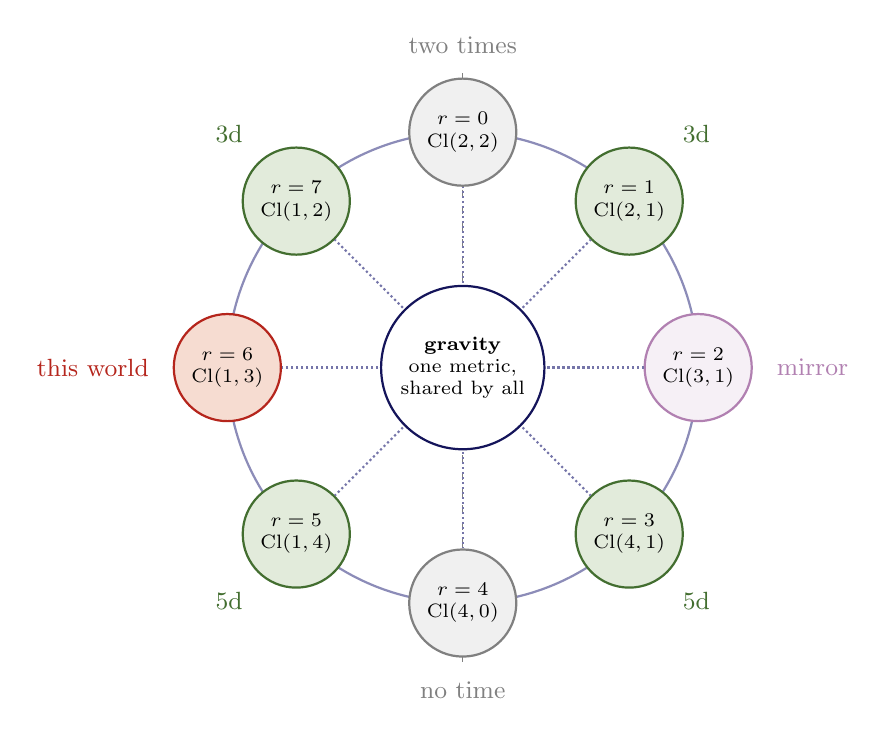
\begin{tikzpicture}[scale=1.15, >=stealth]
\draw[MidnightBlue!50, thick] (0,0) circle (2.6);
\draw[gray, dashed] (0,3.25) -- (0,-3.25);
\foreach \r/\lab/\col/\dims in {
  0/{$r=0$\\$\Cl(2,2)$}/gray/{two times},
  1/{$r=1$\\$\Cl(2,1)$}/OliveGreen!80!black/{3d},
  2/{$r=2$\\$\Cl(3,1)$}/Plum!80!black/{mirror},
  3/{$r=3$\\$\Cl(4,1)$}/OliveGreen!80!black/{5d},
  4/{$r=4$\\$\Cl(4,0)$}/gray/{no time},
  5/{$r=5$\\$\Cl(1,4)$}/OliveGreen!80!black/{5d},
  6/{$r=6$\\$\Cl(1,3)$}/BrickRed/{this world},
  7/{$r=7$\\$\Cl(1,2)$}/OliveGreen!80!black/{3d}}{
  \node[circle, draw=\col, thick, fill=\col!12, minimum size=1.36cm,
        font=\scriptsize, align=center] (n\r) at ({90-45*\r}:2.6) {\lab};
  \node[\col, font=\small, anchor={270-45*\r}] at ({90-45*\r}:3.36) {\dims};
  \draw[MidnightBlue!60, densely dotted, thick] (0,0) -- (n\r);
}
\node[circle, draw=MidnightBlue!80!black, thick, fill=white, minimum size=1.5cm, font=\scriptsize, align=center] at (0,0) {\textbf{gravity}\\one metric,\\shared by all};
\end{tikzpicture}
\caption{The eight towers as the residues of the mod-8 clock (Proposition \ref{prop:residues}), each labelled by its representative under P3, all joined to the one metric at the centre, the only way they touch. Our world is $r = 6$; its mirror $r = 2$, across the dashed axis $r \mapsto -r$, is a copy of it; the grey residues, $r = 0$ with two times and $r = 4$ with none, are sterile, the fixed points of that axis. The odd residues carry no flag bit on any window, the even ones carry it at these P3 representatives (Theorem \ref{thm:paritybit}), so the arrow exists at $r = 6$ and $r = 2$ only.}
\label{fig:clock}
\end{figure}

\begin{definition}[Null blades, the Fock ideal, and chirality]\label{def:fock}
Let $V_{\C}$ be the complexified ambient of a representative, of dimension $2m$ or $2m + 1$, and let $V_{\C} = W \oplus W'$ ($\oplus\, \C\ell$ in odd dimension) be a Witt decomposition into a maximal isotropic subspace $W$ and a dual isotropic complement $W'$, with null bases $w_{1}, \ldots, w_{m}$ of $W$ and $v_{1}, \ldots, v_{m}$ of $W'$ normalised so that $v_{i}w_{j} + w_{j}v_{i} = \delta_{ij}$, and, in odd dimension, an extra unit generator $\ell$ orthogonal to both. The \emph{null blade} of $W$ is $f = w_{1}w_{2}\cdots w_{m}$, and it is annihilated by $W$ from the left: $wf = 0$ for every $w \in W$. The \emph{pseudoscalar} is $I = e_{1}\cdots e_{\dim V}$ for an orthonormal basis, normalised by a fourth root of unity so that $I^{2} = 1$ (the sign of $I$ is a convention; only ratios of its eigenvalues are used below); in even dimension it anticommutes with every vector, in odd dimension it is central. The \emph{Fock ideal} is, in even dimension, the left ideal $S = \Cl(V_{\C})\,f$, spanned by the $2^{m}$ states $v_{i_{1}}\cdots v_{i_{k}}f$ ($i_{1} < \cdots < i_{k}$), the \emph{Fock grade}-$k$ states (counting creation operators, not the Clifford grade); it is the spinor module. In odd dimension the left ideal $\Cl(V_{\C})\,f$ has dimension $2^{m+1}$ and is the sum of the two irreducible modules; the Fock ideal is then either chirality-projected half, $S_{\pm} = \tfrac{1}{2}(1 \pm I)\,\Cl(V_{\C})\,f$, of dimension $2^{m}$, graded by the Fock grade of the projected states $\tfrac{1}{2}(1 \pm I)\,v_{i_{1}}\cdots v_{i_{k}}f$, on which $I$ acts as $\pm 1$ and the extra generator $\ell$ acts as that grade's parity up to a fixed scalar. A state $\psi \in S$ with $I\psi = \pm\psi$ has \emph{chirality} $\pm 1$. For a maximal isotropic subspace $U \subset V_{\C}$, a \emph{pure spinor of $U$} is a nonzero $\psi_{U} \in S$ with $U\psi_{U} = 0$.
\end{definition}

\begin{proposition}[The two families are the two chiralities]\label{prop:families}
In even dimension $2m$:
\begin{enumerate}
\item[(i)] every maximal isotropic $U$ has a pure spinor, unique up to scale, and it is a chirality eigenstate; the pure spinor of $W$ is the null blade $f$ itself, of Fock grade zero, and the pure spinor of $W'$ is the top state $v_{1}\cdots v_{m}f$, of Fock grade $m$;
\item[(ii)] the chirality of $\psi_{U}$ is preserved by even versors (the spin group) and reversed by odd versors (reflections), so the \emph{family} of $U$, defined as the chirality of its pure spinor, is an invariant of the connected isometry group and not of the full one;
\item[(iii)] there are exactly two families, and a Witt pair $W$, $W'$ lies in opposite families if and only if $m$ is odd.
\end{enumerate}
In odd dimension $2m + 1$ there is one family: the connected isometry group acts transitively on maximal isotropic subspaces, and the spin algebra does not preserve the grade parity of $S$.
\end{proposition}

\begin{proof}
(i) Existence for $W$: $w_{i}f = 0$ since $w_{i}$ anticommutes with the other $w_{j}$ and $w_{i}^{2} = 0$. Uniqueness: on the grade-$k$ state $v_{i_{1}}\cdots v_{i_{k}}f$, $w_{j}$ acts as zero if $j \notin \{i_{1}, \ldots, i_{k}\}$ and otherwise, using $w_{j}v_{i} = \delta_{ij} - v_{i}w_{j}$, removes the factor $v_{j}$ up to sign; so the common kernel of $w_{1}, \ldots, w_{m}$ on $S$ is the grade-zero line $\C f$. For $W'$ the same computation with the roles exchanged gives the top state, which every $v_{i}$ annihilates since $v_{i}^{2} = 0$. For a general $U$, Witt's theorem (as in Proposition \ref{prop:flaggable}) supplies an isometry $\rho$ with $\rho(W) = U$, and $\rho$ is the twisted adjoint action of a versor $R$, $\rho(x) = \pm RxR^{-1}$; then $U(Rf) = \pm R(Wf)R^{-1}R = 0$, so $Rf$ is a pure spinor of $U$, and it is the only one up to scale because $R$ is invertible on $S$. Chirality: $I$ commutes with every even element, so $I$ acts on each grade as a scalar; explicitly
\[
I \;\propto\; \prod_{i}(v_{i}w_{i} - w_{i}v_{i}) \;=\; \prod_{i}(2v_{i}w_{i} - 1),
\]
and the $i$-th factor is $-1$ on states without $v_{i}$ and $+1$ on states with it, so the grade-$k$ states have chirality $\epsilon(-1)^{m-k}$ with $\epsilon$ the normalisation; every pure spinor, being a versor image of $f$, is a chirality eigenstate by (ii).

(ii) In even dimension $e_{j}I = -Ie_{j}$ for every basis vector, so $I$ commutes with even versors and anticommutes with odd ones; if $I\psi = \chi\psi$ then $I(R\psi) = \pm R I\psi = \pm\chi(R\psi)$ with the sign that of $R$'s parity.

(iii) Both chiralities occur among pure spinors (reflect $W$ in any non-null vector), chirality is constant on each orbit of the connected group by (ii), and the full isometry group, which is the connected group together with one reflection, is transitive by Witt; so there are exactly two orbits, one per chirality. For the Witt pair, $f$ has grade $0$ and the top state grade $m$, so their chiralities are $\epsilon(-1)^{m}$ and $\epsilon$: opposite exactly when $m$ is odd. Odd dimension: $-1$ is an improper isometry ($\det(-1) = (-1)^{2m+1}$) that fixes every subspace, so every orbit of the full group is an orbit of the connected group, and Witt's transitivity gives one family; and on either half $S_{\pm}$ the extra generator $\ell$ acts as the Fock grade parity up to a scalar (script-checked in dimensions five and seven), while the spin-algebra bivector $e_{1}\ell$ anticommutes with $\ell$, so the spin algebra mixes the Fock grades within each irreducible module.

The script builds $I$, $f$ and the top state on the split real forms of dimensions four, six and eight in \texttt{GA.py} and checks that both are eigenstates of $I$ with eigenvalues in the ratio $(-1)^{m}$ exactly (only the ratio is invariant, the sign of $I$ being a convention; the chiralities agree at $m = 2, 4$ and differ at $m = 3$), that $I$ anticommutes with every generator in even dimension and commutes with every generator in dimensions five and seven, and exhibits the exchanging versors with their parities. The classical result, with the general criterion that two maximal isotropic subspaces lie in one family exactly when their intersection has dimension congruent to $m$ modulo two, is Chevalley's \cite[Ch.~III, \S1]{Chevalley1954}, see also \cite{LawsonMichelsohn1989}; only the Witt-pair case is used here, and it is proved here.
\end{proof}

\begin{theorem}[The flag bit exists exactly at tower dimension $0 \bmod 4$]\label{thm:paritybit}
Let a tower have dimension $n$ and conformal completion with ambient $V$ of dimension $n + 2$, and let $W, W' \subset V_{\C}$ be a Witt pair, the two halves of Definition \ref{def:flag} taken coherently across the pairs, with pure spinors the null blade $f$ and the top state (Definition \ref{def:fock}). Then the choice between $W$ and $W'$ is a discrete invariant of the connected conformal spin group, a \emph{bit}, if and only if $n \equiv 0 \pmod 4$ (ambient dimension $2m$ with $m$ odd), and the bit is the chirality of the pure spinor, that is, the parity of the Fock grade of the complementary half's pure spinor ($0$ for $f$, $m$ for the top state). (i) The odd residues are odd-dimensional for every signature in the class, so the ambient is odd-dimensional, the pseudoscalar central, an even versor carries $W$ to $W'$, and the spin algebra mixes the Fock grades: no bit, on any window. (ii) The even residues carry the bit exactly at tower dimension $0 \bmod 4$: under Premise \ref{prem:window} all four are at dimension four and carry it; the causal representatives of the alternative windows of Proposition \ref{prop:residues}(iii), $(1,1)$ of $r = 0$ and $(1,5)$ of $r = 4$, do not. So the towers that can be oriented are the even residues $\{0, 2, 4, 6\}$ given P3, and the odd residues cannot be, given nothing.
\end{theorem}

\begin{proof}
By Proposition \ref{prop:families}(iii) the Witt pair lies in opposite families exactly when $\dim V_{\C} = 2m$ with $m$ odd, and a choice between $W$ and $W'$ that the connected group cannot undo is exactly a difference of family, since the connected group is transitive within a family (Witt together with Proposition \ref{prop:families}(ii)): so the bit exists if and only if $m$ is odd, and it is the chirality $\epsilon(-1)^{m}$ against $\epsilon$ of the two pure spinors, the Fock-grade parity of the top state $v_{1}\cdots v_{m}f$. With $2m = n + 2$, $m$ is odd if and only if $n \equiv 0 \pmod 4$. For this tower and the mirror, $\dim V_{\C} = 6$, $m = 3$: opposite families, the choice a bit; in ambient dimensions four and eight ($m = 2, 4$: $(1,1)$ and $(1,5)$) the top state has even grade, the same chirality as $f$, and there is no bit.

For odd $n$, $\dim V_{\C}$ is odd and Proposition \ref{prop:families}'s odd case applies: one family, the exchanging even versor exhibited in dimensions five and seven. The script corroborates with the exchanging isometry's determinant, $(-1)^{m}$ in even dimension and $+1$ in odd.

The listing choice of \cite[Prop.~5.6]{ButlerT12} is the choice of which half of each pair annihilates, $f$ against the top state (Definition \ref{def:fock}). That odd residues are odd-dimensional only is $p - q \equiv p + q \pmod 2$, script-checked to dimension ten; a split real form suffices because every statement concerns $V_{\C}$, $S$ and $I$, shared by all real forms with the same complexification.
\end{proof}

\begin{corollary}[Which towers can carry the arrow]\label{cor:whocarries}
The descent's orientation, and with it the asymmetry the flag sets in Proposition \ref{prop:arrow}, is undefined in the odd residues: $1, 3, 5, 7$ cannot be oriented and carry no asymmetry, whatever their content or window. It is defined in the even residues at their P3 representatives, all four-dimensional. Of those, $6$ and $2$ have one time, $4$ has none, and $0$ has two; so the towers that are both oriented and causal are this one and the mirror.

The two-time fork therefore leads to an \emph{oriented} tower: $(2,2)$ has ambient $\R^{3,3}$, $\mathrm{Spin}(3,3) \cong SL(4,\R)$, real four-component twistors, three pairs, mass beginning at two by
\[
\det(\pi^{1}\tilde\pi^{1T} + \pi^{2}\tilde\pi^{2T}) \;=\; \br{\pi^{1}\pi^{2}}\br{\tilde\pi^{1}\tilde\pi^{2}}, \qquad \br{\pi\rho} = \pi_{1}\rho_{2} - \pi_{2}\rho_{1},
\]
for the two real spinor parts of $\mathrm{Spin}(2,2) \cong SL(2,\R) \times SL(2,\R)$, and the Standard-Model gauge algebra by that paper's Proposition 4.3 in dimension four \cite[Prop.~4.3]{ButlerT12}, whose two conditionalities (mass-begins-at-two in dimension $n \neq 4$ as a hypothesis, and the identification of the gauge algebra with the automorphisms of minimal massive compositeness) it carries: a Kleinian copy of the Standard Model. Its share would be one only on two equalities the paper cannot supply off this tower's reversal orbit: the asymmetry per mode (P4, a premise on the fork) and the ceiling coupling (Theorem \ref{thm:mirror}(iv), Proposition \ref{prop:norule}(c)). The two-time instability import keeps the fork closed.
\end{corollary}

\begin{proof}
Theorem \ref{thm:paritybit} with Proposition \ref{prop:residues}(ii); the $(2,2)$ mass identity is Cauchy-Binet on the two $2 \times 2$ matrices $(\pi^{1}\ \pi^{2})$ and $(\tilde\pi^{1}\ \tilde\pi^{2})$, script-checked on exact instances; the gauge algebra is the cited proposition at $n = 4$.
\end{proof}

\begin{remark}[Point of contact: what kind of dark matter this is]\label{rem:whatkind}
The towers are the transport construction's own parallel copies, not a sector added to explain a number. The nearest relatives are mirror matter and asymmetric dark matter \cite{FootMirror2004, Zurek2014}; what the framework adds is that the count, the stability, the mirror's share and the arrow's confinement to the oriented towers are derived from the one descent, which is also what puts them at risk (Section \ref{sec:premises}).
\end{remark}


\begin{remark}[The fork's cost restated: the causal criterion is a theorem, and the bit on the fork is read once]\label{rem:forkrepriced}
The foundations paper proves the causal criterion $\min(p, q) = 1$, a definition in Proposition \ref{prop:residues}, as a theorem about the cone: $\{Q > 0\}$ and $\{Q < 0\}$ have the components of $S^{p-1}$ and $S^{q-1}$, so a future/past split exists exactly in the causal signatures, while $(2,2)$ has an invariant ratio and no arrow \cite[Lem.~4.4(iv)]{ButlerT16}. This does not close the fork of Corollary \ref{cor:whocarries}, sterility being about population; it prices it. Under Hypothesis (S) the descent's bit is read twice, as the asymmetry sign and as the arrow (Proposition \ref{prop:orientation}), and the foundations paper proves the two readings inseparable at $\Cl(1,3)$ level under the same (S) \cite[Cor.~5.7]{ButlerT16}. On the $(2,2)$ fork the bit exists (Theorem \ref{thm:paritybit}) but the arrow does not, so the Kleinian Standard Model would be oriented but timeless: a sharper, algebraic cost than the imported two-time instability.
\end{remark}

\section{Dark, stable, counted}\label{sec:count}

\begin{proposition}[Superselected, hence dark and exactly stable]\label{prop:stable}
By Premise \ref{prem:single} and the acoustic programme (Fact \ref{fact:acoustic}), matter in a neighbouring tower gravitates on this metric and does nothing else: dark by structural necessity. Stability is then not suppressed but exact, in three steps, the first of which is proved given the sector decomposition of Definition \ref{def:frozenops}.
\begin{enumerate}
\item The tower charge $r$ is superselected in the frozen phase: frozen-phase operators are built from the one soldering and preserve its signature (Theorem \ref{thm:soldered}), so portal matrix elements between residues vanish identically away from walls.
\item The walls are unreachable: singular loci ascend within-tower, since the completion adjoins exactly $(1,1)$ and preserves the residue (Fact \ref{fact:towers}), while the mod-8 shadow walls that separate residues are displaced successively away from the physical region, by the wall-sequence theorem of the sheaf paper \cite[\S5]{ButlerT4}, under that theorem's hypotheses (a compact base and good couplings at every stage), carried here.
\item Therefore the only inter-tower event in the universe's history is the descent itself: the towers communicated once, at the origin, and have been in absolute mutual darkness but for weight ever since. The singular locus of a black hole is an inter-tower event for energy, as it already was for weight, and never for the residue of any quantum: energy crosses at the wall, the residue does not (Proposition \ref{prop:infall}).
\end{enumerate}
One residue is flagged at observation level: dark-tower matter crossing this tower's horizons carries superselected charge the four-dimensional boundary mode space cannot hold, which routes it into the tower-wise run of the singularity paper's ascend-then-descend structure \cite{ButlerT5}; the computation of that routing, with the mass range of its Gauss-law clause, is Proposition \ref{prop:infall}.
\end{proposition}

\begin{proof}
(1) Under the sector decomposition of Definition \ref{def:frozenops} every frozen-phase local operator is a section of one tower's soldered bundle and acts within that tower's sector, so its matrix elements between distinct residues vanish: the tower charge is superselected, exactly. The hypothesis cannot be weakened to an algebraic one: an operator straddling two sectors would need a fibrewise map between $(A_{r}, V_{r})$ and $(A_{r'}, V_{r'})$ respecting both solderings, and although such maps exist abstractly (Theorem \ref{thm:soldered}(ii)) none carries $V_{r}$ to $V_{r'}$. The shared metric is not a counterexample: gravity couples through stress-energy, which is built from the soldering and is residue-diagonal. (2) is the two imported theorems at their proved levels, the ascent's residue-invariance (Fact \ref{fact:towers}) and the sheaf paper's conservation of degeneracy. (3) is the conjunction: no operator, no reachable wall, hence no channel; the descent, which built all the towers at once, is the one shared event. This is the series' one-way-door argument run tower-wise, with soldered locality in place of locality.
\end{proof}


\begin{fact}[imported: the inputs of the Standard-Model chain]\label{fact:sminputs}
The derivation of the Standard-Model paper's Sections 3 to 5 uses these data and nothing else: (a) the conformal completion $\Cl(2,4)$ soldered to $V = \R^{2,4}$; (b) the complexification $V_{\C}$, its maximal isotropic subspaces and null blades (the pair count), pair systems and chirality halves (Definition \ref{def:fock}); (c) the even subalgebra $\Cl^{0}(2,4) \cong \Cl(2,3) \cong \Mat(4,\C)$, its spin group $SU(2,2)$, and the twistor space as the ideal $\Cl^{0}(2,4)\,f$ of a self-reverse primitive idempotent, with the helicity form $\bar{\psi}\varphi$ built from the ambient reversion (Clifford conjugation of $\Cl(2,3)$; read on this ideal, not on the null-blade Fock ideal, where at $m = 3$ it vanishes); (d) the mass formula $m^{2} = 2|\br{\pi^{1}\pi^{2}}|^{2}$; (e) the Segre lemma and hypercharge by pair counting; (f) Hypothesis (S) (Fact \ref{fact:flag}); (g) signature-free imports: the Cauchy decomposition, the anomaly coefficients, the Fock representation with its Bogoliubov group; (h) the tractor bundle, whose fibre is the completion's spinor space; (i) the two-kinds-of-action fact (MacDowell-Mansouri does not reach the internal factors, which enter through Yang-Mills functionals whose four-dimensional Hodge star depends on the conformal class alone, the $\theta$-terms being the singularity-surviving remainder); (j) one-loop running, in a conditional remark. \emph{Provenance:} \cite[\S\S2-5]{ButlerT12}, Facts 2.1 to 2.11 and Hypothesis (S); the list is this paper's reading, carried as a hypothesis.
\end{fact}

\begin{theorem}[The mirror tower is a copy of this one]\label{thm:mirror}
Every item of Fact \ref{fact:sminputs} is invariant under the signature reversal $(p,q) \mapsto (q,p)$ that carries this tower's signature $(1,3)$ to the mirror's $(3,1)$ (the proof runs the list item by item; the tractor bundle over a $(3,1)$ conformal structure has ambient $\R^{4,2}$ and the same complexified fibre, Hypothesis (S) has no signature in it, and one-loop running depends on the content alone). Hence:
\begin{enumerate}
\item[(i)] the mirror tower's derived content is a copy of this tower's: gauge algebra $\mathfrak{su}(2) \oplus \mathfrak{su}(3) \oplus \mathfrak{u}(1)$, the same global form, the same generation with the same hypercharges and the same chirality halves, including a massless mirror photon and mirror neutrinos;
\item[(ii)] the ground type (Theorem \ref{thm:types}: $\R$ for the mirror, $\mathbb{H}$ for this tower) does not enter: the derivation uses the conformal spin group and its complex representations, never the tower's real Clifford module;
\item[(iii)] the mirror's light content, and therefore its $\beta$-functions at every scale, equal this tower's, so that with a common ceiling $M$ and a common coupling there its confinement scale and composite spectrum equal ours exactly, $\Lambda_{2} = \Lambda_{6}$ and $c_{2} = c_{6}$, and under P4 its tower factor is $f_{2} = 1$ up to the ratio of mean mass per baryon of the two sectors, which their nuclear histories set (one on the proton-only branch, $0.995$ on the burning branch, Proposition \ref{prop:massbound}(i)): $\Omega_{\mathrm{mirror}} = \Omega_{b}$ to half a percent;
\item[(iv)] the common coupling in (iii) is the one place P2 applies across towers: the reversal is the automorphism of the configuration along whose orbit Premise \ref{prem:indiff} equates, so a coupling difference at the ceiling would be an uncaused distinction between the two members of one orbit, which the audit forbids; the odd towers, off that orbit relative to this one, get no such licence;
\item[(v)] the asymmetry per mode is equal in the two towers, $\epsilon_{2} = \epsilon_{6}$, by two routes, both carried: by the audit, as in (iv), a difference between two continuous data of one reversal orbit being an uncaused distinction; and, more weakly (isomorphic theories share the function, not thereby the value of a datum of theory plus initial condition), by inheritance, both towers being oriented by the one flag under Premise \ref{prem:single}'s orientation clause. So Premise \ref{prem:democracy} is discharged for the mirror, and the share of one in (iii) rests on P1, P2 and the copy.
\end{enumerate}
This is mirror matter in the sense of the literature \cite{FootMirror2004}, derived rather than posited: the framework's $r = 2$ tower is a second Standard Model.
\end{theorem}

\begin{proof}
The list of inputs is Fact \ref{fact:sminputs}, whose own lemmas (pair count, Segre) are statements about $V_{\C}$ and about tensor products of complex spaces. Invariance item by item.

Complexification: $\R^{2,4} \otimes \C = \R^{4,2} \otimes \C$ as quadratic spaces, there being no signature over $\C$. Even subalgebra: $e_{i} \mapsto e_{i}e_{n}$ ($i < n$) identifies $\Cl^{0}(p,q)$ with $\Cl(p, q-1)$ when $e_{n}^{2} = -1$; the script verifies the relations exactly for $(2,4)$ and $(4,2)$, and Theorem \ref{thm:types}'s computation gives $\Cl(2,3)$ and $\Cl(4,1)$ the same type, centre and module dimension, both $\Mat(4,\C)$. The spin group (even versors with $R\tilde{R} = 1$) and the invariant form $\bar{\psi}\varphi$ on $\Cl^{0}f$ are defined by the even subalgebra and the ambient reversion, which the reversal leaves unchanged, since $(p,q) \mapsto (q,p)$ changes the signs of vector squares and not the order of products. Under $e_{i} \mapsto e_{i}e_{n}$ the ambient reversion becomes Clifford conjugation of $\Cl(2,3)$, the antilinear involution a hermitian form needs, and the form so built has signature $(2,2)$: the spin group is $SU(2,2)$ in both cases, with the same twistor representation (likewise $\Cl^{0}(1,3) \cong \Cl(1,2)$ and $\Cl^{0}(3,1) \cong \Cl(3,0)$ are both $\Mat(2,\C)$, with the same Lorentz spin group and Weyl spinors).

Mass formula: $m^{2} = 2|\br{\pi^{1}\pi^{2}}|^{2}$ is the squared norm of $\pi^{1} \wedge \pi^{2}$ for Weyl spinors of the common $SL(2,\C)$. Segre and hypercharge: statements about $\C^{2} \otimes \C^{3}$ and mode counts. Hodge star: on two-forms in four dimensions
\[
(\star F)_{ab} \;=\; \tfrac{1}{2}\sqrt{|g|}\,\epsilon_{abcd}\,g^{ce}g^{df}F_{ef},
\]
even in $g$, so $F \wedge \star F$ and $F \wedge F$ are reversal-invariant.

(i) follows by running the paper's chain on the reversed data; (ii) is the observation that the real module of $\Cl(p,q)$ appears nowhere in the list. (iii): identical content gives identical $\beta$-functions in any scheme, to all orders; with $\alpha_{2}(M) = \alpha_{6}(M)$ the running solutions coincide, so $\Lambda_{2} = \Lambda_{6}$, and the composite spectra, being those of isomorphic theories, coincide, $c_{2} = c_{6}$; then, under P4,
\[
f_{2} \;=\; \frac{\epsilon_{2}}{\epsilon}\cdot\frac{n_{2}}{n_{6}}\cdot\frac{m_{2}}{m_{6}} \;=\; 1 \cdot 1 \cdot 1 .
\] (iv) is the audit clause of Premise \ref{prem:indiff} read in the direction it permits.
\end{proof}

\begin{theorem}[Mode counts: two modules, and which one the series' matter lies in]\label{thm:modes}
Let the towers be populated at a common rung height $k$ (one descent, P1). The tower paper's Fock module of tower $r$ at that height is $S_{r} \otimes \mathcal{F}_{k}$, the ground spinor module tensored with the Fock space of the $k$ ladder pairs, with $\tfrac{1}{2}\dim_{\R} S_{r} \cdot 2^{k}$ fermionic modes; the Standard-Model paper's derived matter is a different object, the state space $\Lambda^{\bullet}(\C^{2} \oplus \C^{3})$ of five twistor modes, built from the conformal spin group alone (Theorem \ref{thm:mirror}(ii)). Then:
\begin{enumerate}
\item[(i)] the rung factor does not depend on the residue: every populated P3 representative has Witt index $\min(p,q) = 1$, so the capacity at height $k$ is $1 + k$ in every tower \cite[Thm.~4.3]{ButlerT3} and the Fock factor $\mathcal{F}_{k}$ has dimension $2^{k}$ in every tower;
\item[(ii)] the ground factor is not: with both irreducible modules counted where the centre splits (Premise \ref{prem:indiff}: selecting one of two inequivalent modules by the sign of the volume element would be an uncaused choice), $\dim_{\R} S_{r}$ is $8$ at $r = 6$, $4$ at $r = 2$, $4$ at $r = 1$, $4$ at $r = 7$, $8$ at $r = 3$ and $16$ at $r = 5$; with one module each, $2$ at $r = 1$ and $8$ at $r = 5$;
\item[(iii)] hence the ground-module weighting of the five dark towers' Fock modes relative to this one's, in the labelling convention of Proposition \ref{prop:residues}, is
\[
\sum_{r \neq 6} \frac{n_{r}}{n_{6}} \;=\; \frac{1}{2} + \frac{1}{2} + \frac{1}{2} + 1 + 2 \;=\; \frac{9}{2} \qquad\text{(both modules)},\qquad\text{or}\qquad \frac{13}{4}\ \text{(one module each)},
\]
and in the opposite convention, where this world is the $4$-dimensional real module and the mirror the $8$-dimensional quaternionic one, $40/4 = 10$ and $30/4 = 15/2$: the weighting depends on the convention because it divides by a named member's module, and it counts modes, not anything that enters an asymmetric sum (Corollary \ref{cor:whocarries});
\item[(iv)] but the series' matter is the derived state space, not the full Fock module, and the mirror's is identical to this tower's (Theorem \ref{thm:mirror}), so $n_{2} = n_{6}$ and the mirror's weight is $1$, not $\tfrac{1}{2}$; for the odd towers the state space needs the twistor correspondence in dimensions three and five, which the series establishes only in four \cite{ButlerT9}, so $n_{1,7,3,5}$ are not determined here beyond the pair counts $2$ (three dimensions) and $3$ (five), and they do not enter the asymmetric count, the odd towers carrying no asymmetry.
\end{enumerate}
The $9/2$ (or $10$) of (iii) is the value of a computation in a convention, not the count, by (iv).
\end{theorem}

\begin{proof}
(i) is $\min(p,q) = 1$ for each of $(1,3)$, $(3,1)$, $(2,1)$, $(1,2)$, $(4,1)$, $(1,4)$, read off, and the tower paper's theorem that the Witt index rises by exactly one per rung. (ii): for $\Cl(p,q) \cong \Mat(m, D)$,
\[
\dim_{\R} S \;=\; m \dim_{\R} D, \qquad m \;=\; \sqrt{\frac{2^{n}}{c\,\dim_{\R} D}},
\]
with $c$ the number of simple components; $D$ and $c$ are Theorem \ref{thm:types}, and the script computes $m$ and $\dim_{\R} S$ for each P3 representative from its own exact determination of $D$ and $c$, returning the values listed. (iii) is the arithmetic of (ii) divided by $8$, and by $4$ in the other convention, script-checked as exact rationals. The identification of the tower's Fock module as $S_{r} \otimes \mathcal{F}_{k}$ is the tower paper's Fock-module theorem for the factor $\mathcal{F}_{k}$ and its commuting-copies theorem for the tensor factorisation with the ground module \cite[Thms.~4.2 and 3.2]{ButlerT3}, imported. (iv): the mirror equality is Theorem \ref{thm:mirror}(i); the odd pair counts are the pair-count lemma's maximal isotropic dimension $\lfloor (n+2)/2 \rfloor$ of $V_{\C}$ for $n = 3, 5$, with the script exhibiting that many orthogonal null vectors and the bound $\dim U^{\perp} = \dim V - m$ (the value is the formula's, the witnesses the script's); the scope statement is the twistor paper's own (four dimensions).
\end{proof}

\begin{proposition}[The population count: one share to half a percent, and a symmetric remainder]\label{prop:count}
For an oriented residue $r$ write $\epsilon_{r}$ for the asymmetry per mode, $n_{r}$ for the mode count of its derived matter and $m_{r}$ for the mass per unit of asymmetry, and
\[
f_{r} \;=\; \frac{\epsilon_{r}\,n_{r}\,m_{r}}{\epsilon_{6}\,n_{6}\,m_{6}}
\]
for the tower factor. Under Premises \ref{prem:single}-\ref{prem:democracy}, with every tower's matter diluting as this one's (Lemma \ref{lem:projection}):
\begin{enumerate}
\item[(i)] \emph{(Asymmetric.)} The asymmetric dark matter is the mirror tower's alone (Corollary \ref{cor:whocarries}: the odd towers carry none; residues $0$ and $4$ are sterile), and its share is exactly one (Theorem \ref{thm:mirror}(iii), assembled with its premises in Theorem \ref{thm:share}):
\begin{equation}\label{eq:ratio}
\frac{\Omega^{\mathrm{asym}}_{\mathrm{dark}}}{\Omega_{b}} \;=\; f_{2} \;=\; 1, \qquad\text{against the observed}\qquad \frac{\Omega_{c}}{\Omega_{b}} \approx 5.364 \pm 0.065,
\end{equation}
the one holding to half a percent on the burning branch (Proposition \ref{prop:massbound}(i)).
\item[(ii)] \emph{(Symmetric.)} The remainder, $4.364\,\Omega_{b}$, that is $\Omega h^{2} = 0.0976 \pm 0.0012$, is not asymmetric relic of anything in the framework. An odd tower's matter, if any, is what the descent deposited, heated afterwards only through gravity, the one channel superselection leaves open (Proposition \ref{prop:stable}, Appendix \ref{app:seeding}): a symmetric relic whose density is set by the sector's own dynamics (its lightest stable state, its number-changing rates, its temperature relative to ours), not by a conserved number.
\item[(iii)] \emph{(Scope: the remainder is not derived here.)} No rule relating an odd tower's dimensionful coupling to this tower's dimensionless one follows from the series (Proposition \ref{prop:norule}), and this paper supplies none: its derived claim on the ratio is the one share of (i). What it says about the remainder is the unit-ball rule of Section \ref{sec:rule}, a fitted relation at observation level on three premises of its own, returning $4.364$ as $2 \cdot \tfrac{4}{3} + 2 \cdot \tfrac{8}{3\pi}$; nothing in this proposition depends on it. Beyond this the framework fixes only a floor on the odd towers' temperature, from gravitational heating after the descent (Appendix \ref{app:seeding}: about three and a half parts in ten thousand of ours at the ceiling reheating for a nine-vector content, the deposit possibly more), which closes their radiation channels near the floor and says nothing about their matter density; supplying the coupling rule is successor problem (3).
\end{enumerate}
The profile: the mirror's dark matter is mirror baryons at the proton mass, cold and dissipative within its own sector; the odd towers' is symmetric, of undetermined mass; both couple to this tower by gravity alone. Two conditional stances are registered at the premises' level: permanent null results in direct detection, and no indirect-detection signal from dark decays or visible annihilation products. Observation level on the flagged premises; the observed ratio is the survey record's \cite{Planck2018}.
\end{proposition}

\begin{proof}
(i) is Theorem \ref{thm:mirror}(iii) with Corollary \ref{cor:whocarries} removing the odd towers from the asymmetric sum; $5.364 - 1 = 4.364$ and $4.364 \times 0.02237 = 0.0976$ are script-checked, with the survey uncertainties propagated as rational brackets. (ii) is the definition of a symmetric sector. (iii) is a scope statement resting on Corollary \ref{cor:whocarries} and Proposition \ref{prop:norule}; the rule it points to is used nowhere in this section and it asserts nothing about the remainder's value. The profile is Theorem \ref{thm:mirror}(i) for the mirror and Proposition \ref{prop:stable} for the coupling; the two stances follow from exact superselection and are costed in Section \ref{sec:premises}.
\end{proof}

\begin{proposition}[The stored asymmetry is a charge, not a number]\label{prop:charge}
Under the classification of Proposition \ref{prop:arrow}, with $\epsilon$ initial data of the descent, inherited rather than generated, and the boundary mode count $N$ common to the towers under P1:
\begin{enumerate}
\item[(i)] \emph{(Charge.)} The asymmetry stored in an oriented tower is the charge $Q = \epsilon N$, fixed by the descent's data and independent of the tower's temperature; it is not a thermal number $n - \bar{n} \propto g\,\mu T^{2}$. So the mirror share $f_{2} = 1$ holds at any mirror temperature: a cold mirror carries the same baryon charge as this tower in the same number of baryons, with negligible mirror radiation.
\item[(ii)] \emph{(Origin.)} The charge is the descent's and cannot be produced afterwards: the one channel superselection leaves open, gravitational production from the visible plasma (Appendix \ref{app:seeding}), yields $1.8$ to $2.7 \times 10^{-15}$ mirror quanta per unit entropy at the ceiling reheating against the $8.7 \times 10^{-11}$ baryons per unit entropy that our baryon number requires, more than four orders too few even counting every produced quantum as a baryon. Black holes are a sink for $Q$, not a source (Proposition \ref{prop:infall}(iv), under P5): a mass-preserving rearrangement that erodes each tower's free baryon count and moves no share.
\item[(iii)] \emph{(Temperature.)} The mirror's temperature ratio $\xi = T'/T$ is a datum of the descent, bounded below by the gravitational floor, $\xi$ between $2.8$ and $3.2 \times 10^{-4}$ at the ceiling reheating (Proposition \ref{prop:coefficients}(ii), the bracket the species-counting ambiguity; four parts in a thousand of this at the bottom of the ceiling range), and above by the $\Neff$ cap at $0.448$; a deposit of each unit of baryon number with energy of order the reheating temperature puts it at $\xi \approx 4 \times 10^{-3}$. The paper carries the whole interval. With $\eta = n_{B}/n_{\gamma} = 6.1 \times 10^{-10}$ here and equal baryon number,
\[
\eta' \;=\; \frac{\eta}{\xi^{3}}
\]
runs from $19$ to $26$ at the floor down to about $0.008$ at the hot deposit, crossing one at $\xi = \eta^{1/3} = 8.5 \times 10^{-4}$: at least $10^{7}$ times ours throughout, with $\Delta\Neff$ eight orders or more below the cap.
\item[(iv)] \emph{(The two readings.)} The thermal reading would give $f_{2} \sim \xi_{2}^{3}$ instead, at most $0.090$ under the $\Neff$ cap ($0.448^{3}$) and $10^{-7}$ or less anywhere in the interval; the two readings cannot both hold, and the paper's own classification decides for the charge.
\end{enumerate}
Level: the classification is Fact \ref{fact:trichotomy}'s; the incompatibility is arithmetic. The mirror's nucleosynthesis, which is not a copy of ours and on which the burning branch of Proposition \ref{prop:massbound}(i) and the composition caveat of refutation item 6 rest, follows the proof, at assembly level.
\end{proposition}

\begin{proof}
$f_{2} = (\epsilon_{2}/\epsilon)(n_{2}/n_{6})(m_{2}/m_{6})$ (Theorem \ref{thm:mirror}(iii)) has no temperature in it; $\eta = 2.74 \times 10^{-8}\,\Omega_{b}h^{2}$ and its cube root are script-evaluated. The yield comparison is Proposition \ref{prop:gravseed}'s $Y$ at the ceiling against $\eta$ times the photon-to-entropy ratio $0.1413$. The floor is Proposition \ref{prop:coefficients}(ii); the hot-deposit value is the energy fraction $3\,(n_{B}/s)\,T_{\mathrm{desc}}/(\rho/s)$ with $\rho/s = \tfrac{3}{4}T$, converted to $\xi$ as in Proposition \ref{prop:gravseed}. The nucleosynthesis arithmetic compares
\[
\Gamma_{\mathrm{weak}} \;\approx\; G_{F}^{2}T'^{5} \qquad\text{against}\qquad H \;=\; \frac{1.66\sqrt{g_{*}}\,T'^{2}}{\xi^{2}M_{\mathrm{Pl}}}
\]
(non-reduced $M_{\mathrm{Pl}}$) and solves for the crossing at both ends of the interval; it iterates
\[
\frac{B_{D}}{T'} \;=\; \ln\frac{1}{\eta'} + \frac{3}{2}\ln\frac{m_{p}}{T'}
\]
to a fixed point for the bottleneck; and it evaluates the entropy-evolution factor
\[
(g_{\mathrm{mir}}^{\mathrm{seed}}/g_{\mathrm{mir}})^{1/3}(g_{\mathrm{vis}}/g_{\mathrm{vis}}^{\mathrm{seed}})^{1/3},
\]
the photon energy per baryon $2.701\,T'/\eta'$ with the plasma budget $2.75$ times it, the completion-limit reheating factor $(1 + 7.07\ \mathrm{MeV}/E_{\mathrm{plasma}})^{1/4}$, the density and cosmic time at the bottleneck and the Saha recombination temperature, all script-bracketed in decimal arithmetic. The burning itself (the standard network at a baryon density eleven orders above ours, with photodisintegration active at the reheated temperature) is assembly level, a branch with its completion limit, not derived.
\end{proof}

\medskip\noindent\textbf{Discussion of Proposition \ref{prop:charge}: the interval, and the mirror's nucleosynthesis.} The paper's own mechanism favours the hot end (the tower charges are created at the freezing in quanta of order the reheating temperature), but the nucleosynthesis is computed at the floor, the one value the framework fixes, the hot end being the trivial case; the interval straddles the crossover of $\eta'$ at one, charge-dominated below it, and statements that hold only at the charge-dominated end are labelled ``at the floor''.

\smallskip\noindent\emph{Weak freeze-out and the burning branch.} The mirror's expansion rate is set by the visible plasma at $T = T'/\xi$, so its weak rate over the Hubble rate scales as $T'^{3}$: at the floor it crosses one at $T' \approx 0.43$ to $0.45$ GeV, above the mirror's QCD crossover at $155$ MeV At the floor the mirror's weak interactions froze out with its quarks free and the up-down ratio thermal (at the hot end the crossing falls below $100$ MeV, under the crossover but still where $n/p \approx 1$), so the neutron-to-proton ratio at hadronisation is near one and burning is the framework's expectation. A proton-only mirror would need a mirror lepton asymmetry large enough to bias that ratio, a datum the framework does not fix; it is carried as the alternative branch.

\smallskip\noindent\emph{The bottleneck and the reheat, at the floor.} The deuterium bottleneck opens near $T' = 0.23$ to $0.24$ MeV, not at our $0.062$, at a baryon density of $0.8$ to $1.2 \times 10^{31}\ \mathrm{cm^{-3}}$ and a cosmic time of microseconds, so mirror neutrons cannot decay first and whatever can burn, burns (by then $T'/T$ has risen by about $2.6$ from its seeded value through the two sectors' separate entropy conservation, leaving $\eta'$ within ten percent). The released $7.07$ MeV per nucleon enters a plasma carrying $25$ to $33$ keV of photon energy per baryon and $2.75$ times that with pairs (thermal pairs at zero chemical potential, a lower bound on the budget, so the reheating factor below is an upper bound), so complete burning would reheat the mirror by $3.0$ to $3.2$, to $T' \approx 0.70$ to $0.78$ MeV and $\eta' \approx 0.72$ to $0.81$. Photodisintegration makes the endpoint a nuclear-statistical-equilibrium problem that completes only as expansion cools it; the figures are the completion limit. At the hot end burning does not reheat the mirror appreciably.

\smallskip\noindent\emph{Recombination, and the caveat on imported bounds.} On the burning branch the mirror is helium. It recombines earlier than we do because its photons are fewer, at $T'$ between about $0.55$ eV at the hot end and $0.68$ eV at the floor after its burning ($0.85$ eV on the proton-only branch, and higher still for helium), at a visible temperature between $0.1$ and $0.8$ keV across the interval. So bounds derived for a mirror sector with our $\eta$ assume a baryon-to-photon ratio, and on the burning branch a composition, nothing like the mirror's; the mirror-galaxy analysis of refutation item 6 rescales $\eta'$ and includes a helium mirror, but only at the hot end of the interval.


\begin{proposition}[The mirror share is one, and how fragile that is]\label{prop:massbound}
Write $m_{r} = c_{r}\Lambda_{r}$, with $\Lambda_{r}$ the confinement scale of tower $r$'s non-abelian sector and $c_{r}$ the constituent factor of its lightest charge-carrying composite.
\begin{enumerate}
\item[(i)] \emph{(The mirror.)} By Theorem \ref{thm:mirror}(iii), $\Lambda_{2} = \Lambda_{6}$ and $c_{2} = c_{6}$ exactly, hence $f_{2} = 1$ under P4, an isomorphism of theories rather than a one-loop statement. As a ratio of mass densities it is a ratio of mean mass per baryon: ours is about $936.7$ MeV after helium, a mirror burnt entirely to helium (the completion limit of Proposition \ref{prop:charge}'s burning branch) gives $931.8$ MeV, so $f_{2}$ is $0.995$ in that limit and $1$ on the proton-only branch, a one-sided systematic of half a percent at assembly level.
\item[(ii)] \emph{(Fragility.)} The equality is unstable to any departure from the copy. Suppose the two towers shared a ceiling $M$ and coupling but differed in light content by $\Delta b$ over the running range, with $b_{6} \leq 11$; then at one loop
\[
\ln\frac{\Lambda_{2}}{\Lambda_{6}} \;\geq\; \frac{\Delta b}{b_{6} + \Delta b}\,\ln\frac{M}{\Lambda_{6}}.
\]
One Dirac flavour is $\Delta b = 2/3$, which with $\Lambda_{6} = 0.3$ GeV moves the mirror share by a factor between $4.89$ (bottom of the ceiling range, $b_{6} = 11$) and $21.4$ (top, $b_{6} = 7$), past the observed $5.364$ everywhere except at the bottom of the range on the most conservative branch. A coupling departure $\delta = \alpha_{2}(M)^{-1} - \alpha_{6}(M)^{-1}$ at the ceiling with identical content moves $\Lambda_{2}/\Lambda_{6}$ by $e^{-2\pi\delta/b}$, a factor $2.45$ per unit at $b = 7$, so the share stays within ten percent of one only for $|\delta| < 0.106$. So $f_{2} = 1$ is exact, P2-protected, and fragile.
\item[(iii)] \emph{(The odd towers.)} In three and five dimensions the gauge coupling is dimensionful and the confinement scale is set by the coupling itself ($\Lambda_{3} \sim g_{3}^{2}N$, $\Lambda_{5} \sim 1/g_{5}^{2}$), so nothing about $\Lambda_{1,7,3,5}$ follows without a rule the series does not derive (Proposition \ref{prop:norule}); the unit-ball rule of Section \ref{sec:rule} constrains that rule, as shares per unit of our volume, without supplying it.
\end{enumerate}
Level: (i) is Theorem \ref{thm:mirror}; (ii) is one-loop arithmetic under its stated assumptions, flagged; (iii) is a scope statement.
\end{proposition}

\begin{proof}
(i) is Theorem \ref{thm:mirror}(iii). (ii): one loop,
\[
\alpha(\mu)^{-1} \;=\; \alpha(M)^{-1} - \frac{1}{2\pi}\int_{\mu}^{M} b\,d\ln\mu'
\]
for an asymptotically free sector, with $\Lambda$ the scale at which $\alpha^{-1}$ vanishes. With equal $\alpha(M)^{-1}$ and $b_{2} - b_{6} \geq \Delta b$,
\[
\alpha_{2}(\mu)^{-1} \;\leq\; \alpha_{6}(\mu)^{-1} - \frac{\Delta b}{2\pi}\ln\frac{M}{\mu};
\]
at $\mu = \Lambda_{2}$ the left side vanishes, so
\[
\frac{\Delta b}{2\pi}\ln\frac{M}{\Lambda_{2}} \;\leq\; \alpha_{6}(\Lambda_{2})^{-1} \;\leq\; \frac{b_{6}^{\max}}{2\pi}\ln\frac{\Lambda_{2}}{\Lambda_{6}}.
\]
Writing $L = \ln(\Lambda_{2}/\Lambda_{6})$ and $L_{0} = \ln(M/\Lambda_{6})$,
\[
b_{6}^{\max}L \;\geq\; \Delta b\,(L_{0} - L), \qquad\text{so}\qquad L \;\geq\; \frac{\Delta b\,L_{0}}{b_{6}^{\max} + \Delta b};
\]
the script checks the chain as exact rational algebra and evaluates the factors at both ends of the ceiling range ($L_{0} = 35.23$ and $27.79$; $7.49$, $21.4$ at the top and $4.89$, $11.2$ at the bottom for $\Delta b = 2/3$; $18.84$ for $\Delta b = 1$). The coupling sensitivity is $\Lambda = M e^{-2\pi/(b\alpha(M))}$ differentiated, $d\ln\Lambda/d(\alpha^{-1}) = -2\pi/b$. (iii) is dimensional analysis: $[g^{2}] = \text{mass}^{4-d}$.
\end{proof}


\begin{theorem}[The mirror share, assembled]\label{thm:share}
Under Premises \ref{prem:single}, \ref{prem:indiff} and \ref{prem:democracy}, the Standard-Model paper's Hypothesis (S) as carried in Fact \ref{fact:flag}, and the input list of Fact \ref{fact:sminputs}, the mirror tower contributes exactly one visible share:
\[
f_{2} \;=\; \underbrace{\frac{\epsilon_{2}}{\epsilon_{6}}}_{\text{P2}}\cdot\;\underbrace{\frac{n_{2}}{n_{6}}}_{\text{derived}}\;\cdot\;\underbrace{\frac{m_{2}}{m_{6}}}_{\text{derived, given P2}} \;=\; 1\cdot 1\cdot 1 \;=\; 1, \qquad \Omega_{\mathrm{mirror}} \;=\; \Omega_{b},
\]
exactly on the proton-only branch and to half a percent on the burning branch (Proposition \ref{prop:massbound}(i)). The three factors are stated separately because they have three standings, and the exposure of the share is the weakest of them.
\begin{enumerate}
\item[(i)] \emph{(The mode ratio: derived, on no premise of this paper.)} $n_{2} = n_{6}$, the same state space.
\item[(ii)] \emph{(The mass ratio: derived, given P2.)} $m_{2} = m_{6}$ up to the two sectors' composition, the common ceiling coupling being P2 along the reversal orbit.
\item[(iii)] \emph{(The asymmetry ratio: premised on P2.)} $\epsilon_{2} = \epsilon_{6}$ by the audit along the same orbit (P1's orientation clause a weaker second route); P4 is discharged for the mirror, not assumed.
\item[(iv)] \emph{(No temperature in it.)} The share is one anywhere in the interval of Proposition \ref{prop:charge}(iii).
\end{enumerate}
\end{theorem}

\begin{proof}
The product is the tower factor of Proposition \ref{prop:count} evaluated at $r = 2$. (i) Fact \ref{fact:sminputs} lists the data the Standard-Model chain consumes and Theorem \ref{thm:mirror} shows each invariant under the reversal, so the mirror's derived content is this tower's, the ground type never entering (Theorem \ref{thm:mirror}(i), (ii)), and $n_{2}/n_{6} = 1$ (Theorem \ref{thm:modes}(iv)); this uses Fact \ref{fact:sminputs} and Hypothesis (S), and no premise of this paper. (ii) Identical content gives identical $\beta$-functions in any scheme and to all orders, so the common ceiling coupling, Premise \ref{prem:indiff} along the reversal orbit (Theorem \ref{thm:mirror}(iv)), gives $\Lambda_{2} = \Lambda_{6}$ and $c_{2} = c_{6}$; what remains of $m_{2}/m_{6}$ is the ratio of mean mass per baryon, $0.995$ in the helium completion limit and $1$ on the proton-only branch (Proposition \ref{prop:massbound}(i)). (iii) is Theorem \ref{thm:mirror}(v), first route. (iv) $Q = \epsilon N$ is a charge of the descent, $N$ common under P1, and no factor depends on $\xi$ (Proposition \ref{prop:charge}(i)); the thermal reading is excluded by that classification, not by this proof (Proposition \ref{prop:charge}(iv)). With the dilution of Lemma \ref{lem:projection}, common to the towers, $\Omega_{\mathrm{mirror}} = f_{2}\,\Omega_{b} = \Omega_{b}$.

Level: (i) proved given Fact \ref{fact:sminputs} and Hypothesis (S); (ii) proved given (i) and Premise \ref{prem:indiff}, the half percent at assembly level; (iii) premised on Premise \ref{prem:indiff}; (iv) proved given the classification of Proposition \ref{prop:arrow}. Proposition \ref{prop:massbound}(ii) prices any departure from (i).
\end{proof}

\begin{remark}[What the share is exposed to, and what it is not]\label{rem:shareexposure}
Every factor of Theorem \ref{thm:share} is a ratio between two towers, so the share is one whatever content $X$ the Standard-Model chain produces from Fact \ref{fact:sminputs}, correct or not: the reversal carries $X$ to $X$. It is exposed instead to that list's completeness and to P2: a non-invariant input off the list breaks the copy, priced by Proposition \ref{prop:massbound}(ii). The record's test is refutation item 6.
\end{remark}

\begin{observation}[Which towers are populated]\label{obs:population}
The census says which towers can hold matter; it does not say which the descent filled, and the two are at different levels. This tower is populated by observation. The mirror is populated by P2: residues $6$ and $2$ are equivalent under signature reversal, so a descent that filled one filled the other, at the same asymmetry (Theorem \ref{thm:mirror}(v)); this is the one case in which population is derived. The four odd towers are reached by nothing in the series: P2 does not equate them with this tower, the tower paper gives them algebras and not contents, and what the descent deposited in each is the pre-descent theory's, successor problem (2). What supports their population is the record read inside the framework: with the mirror's share exactly one, an empty set of odd towers would make the ratio $1$ against the observed $5.364$, and the framework has no other dark candidate, so, granted the framework, the observed remainder is the evidence that the odd towers hold matter. That is an inference at observation level, not a count, and it is what the unit-ball rule presupposes when it sums over six towers (Premise \ref{prem:R2}). Nothing derived in this paper depends on the odd towers being populated: the mirror share, the superselection, the parity theorem and the arrow are the same if they are empty, and refutation item 6 says so.
\end{observation}

\section{The arrow counted}\label{sec:arrow}

\begin{proposition}[The asymmetry: the arrow counted, and the fifteenth refutation]\label{prop:arrow}
The framework does not generate its asymmetry; it inherits it.
\begin{enumerate}
\item[(i)] \emph{(Sakharov.)} The Sakharov conditions are for generating an asymmetry dynamically from a symmetric state; a universe whose asymmetry is initial data does not need them. The descent supplies the reason the initial data need not be symmetric: it is irreversible (the lossy projection of the taxonomy paper's descent theorem \cite{ButlerT1}), it creates the tower charges, and it makes one orientation choice, the Witt flag, which is what particle-versus-antiparticle means (Fact \ref{fact:flag}). Each matches a Sakharov condition in name; none is a mechanism producing a number.
\item[(ii)] \emph{(The fifteenth refutation.)} A pre-descent $\theta$-term would source asymmetry through the topology of gauge bundles; but it integrates a characteristic class, of even degree, so the odd-dimensional towers carry no continuous $\theta$, and a $\theta$-term exists exactly where a flag bit does. In this tower it is excluded empirically: a $\theta$-routed asymmetry needs an angle of order one at the descent that does not relax before it acts, and the neutron dipole bound $|d_{n}| < 1.8 \times 10^{-26}\,e\,$cm \cite{Abel2020} gives $|\theta| \lesssim 10^{-10}$ today (through a hadronic matrix element with its own uncertainty). Not excluded, and not claimed: an angle that relaxes or rolls; and the mirror's angle, which equals ours only by P2 along the reversal orbit (Theorem \ref{thm:mirror}(iv)), the copy being of the functional, not its coefficient. Internally the paper says only that the orientation is the one mechanism the framework itself supplies; that locates the mechanism and does not refute the alternative.
\item[(iii)] \emph{(Confinement and universality.)} The orientation route is one bit spent once (uniqueness among all conceivable mechanisms is not claimed). A flag exists on every rung of every tower (Remark \ref{rem:flaglives}), but the flag \emph{bit} only in the even residues at their P3 representatives (Theorem \ref{thm:paritybit}), so the asymmetry is confined to the oriented causal towers, this one and the mirror, and the odd towers carry none by either route. Universality of the value is Premise \ref{prem:democracy}, a theorem for the mirror (Theorem \ref{thm:mirror}(v)) and not extendable to inequivalent towers, the asymmetry per mode depending on the tower's own charge structure.
\item[(iv)] \emph{(The value, a stance.)} $\epsilon$ is not derived here and not classified. The trichotomy's kinematic clause runs for it as for $N$ ($\epsilon$ is continuous), at that Fact's observation level; the dynamical clause does not, since generating an asymmetry from CPT-invariant dynamics is exactly what the Sakharov mechanism does. \emph{Stance, flagged and attacked in Section \ref{sec:premises}:} the framework inherits its asymmetry, and $\epsilon$ is initial data of the descent, refuted by any in-framework calculation that produces $\epsilon$ dynamically. The count uses only the equality of $\epsilon$ across the reversal orbit (Theorem \ref{thm:mirror}(v)), not its provenance. On the stance the unexplained numbers are two, $N$ and $\epsilon$, with the orientation bit of Proposition \ref{prop:orientation} a third datum of the same event.
\end{enumerate}
\end{proposition}

\begin{proof}
The refutation in (ii) is a degree count. A $\theta$-term integrates over the tower's space a characteristic class of the gauge bundle ($\tr F \wedge F$ in four dimensions); Chern and Pontryagin classes have even degree, so in odd dimension there is no top-degree class and no continuous $\theta$. Homotopy agrees: bundles on $S^{d}$ are classified by $\pi_{d-1}(G)$, zero in three dimensions ($\pi_{2}(G) = 0$), and in five $\pi_{4}(SU(2)) = \mathbb{Z}_{2}$ allows only a discrete angle, $0$ or $\pi$, with $\pi_{4}(SU(n)) = 0$ for $n \geq 3$; the odd-dimensional Chern-Simons term is a quantised level, not an angle. (iii) is Theorem \ref{thm:paritybit} with Premise \ref{prem:democracy} and Theorem \ref{thm:mirror}(v); (iv) is Fact \ref{fact:trichotomy}(1) at its level, $\epsilon$ being continuous. The degree computation is recorded in the script.
\end{proof}

\begin{proposition}[The orientation is the arrow: the seventeenth refutation]\label{prop:orientation}
The Standard-Model paper left one absolute bit undetermined, the particle-antiparticle orientation, expected to be fixed by the charge-zero condition. The expectation is refuted by a $\mathbb{Z}_{2}$ covariance argument parallel to the trichotomy's rescaling one, on three premises: that CPT conjugation is an isomorphism of every kinematic structure (checked in the proof for the metric, the completion, the pairing and the action; premised for the imported gauge sector and for structures later papers add); Hypothesis (S), under which the Standard-Model paper's chirality proposition, the source of the relative-versus-absolute split, is proved (Fact \ref{fact:flag}); and, for the last step only, the trichotomy's exhaustiveness (Fact \ref{fact:trichotomy}(3)).

Anything the structures determine is conjugation-invariant, and the orientation is not. The charge-zero condition fixes all \emph{relative} structure \cite[Prop.~5.6]{ButlerT12}; the absolute bit is kinematically underdetermined, untouched by the CPT-symmetric action, hence initial data, and it is the Witt flag of Proposition \ref{prop:arrow}: the open orientation of the content derivation and the arrow of time are one choice, made once.

The descent measure carries two numbers and one bit. The neutrino sector supplies no orientation refutation condition: the identification of $\nu_{R}$ with the hypercharge-zero singlet at grade zero is flag-covariant (the conjugate flag exchanges the singlet grades zero and three), so no completion of the orientation could exclude it \cite{ButlerT15}.

This is the seventeenth refutation (the sixteenth is the neutrino paper's \cite[Prop.~4.1(1)]{ButlerT15}), in the pattern of the thirteenth and the trichotomy: what the framework cannot determine, it can prove it cannot determine, and locate.
\end{proposition}

\begin{proof}
CPT conjugation acts on each tower's Clifford bundle as the composition of grade involution, reversal, and the flag conjugate $v_{k} \leftrightarrow w_{k}$ (Definition \ref{def:flag}); the grade involution negates every vector, the timelike one included (the T; the spatial inversion is the P). Structure by structure: the fibre metric is fixed by grade involution, reversal and the exchange of a null pair, which is an isometry of the completion's hyperbolic plane; the pairing on the Fock module sends the grade-$k$ state to the grade-$(3-k)$ state \cite[Prop.~5.6]{ButlerT12}, which is exactly what the flag conjugate does; and the action is the frozen point's, built from the metric and the completion. The derived gauge sector (Fact \ref{fact:sminputs}) is CPT-even by the standard theorem for local Lorentz-invariant actions, but that theorem concerns the antiunitary CPT operator of quantum field theory, whereas the composite here is a real linear $\mathbb{Z}_{2}$ automorphism of the kinematic data, which is not that operator (Wigner). The argument uses only the automorphism, which is checked; the gauge sector's CPT-evenness is imported and carried as a premise.

So conjugation is an automorphism of the kinematic data exchanging the flag's two orientations; a quantity the structures determine would be fixed by it, and the orientation is not; hence no kinematic or dynamical result determines it, and, if the trichotomy is exhaustive (the third premise), it is initial data. The relative-versus-absolute split is the Standard-Model paper's chirality proposition, imported under Hypothesis (S); the flag-covariance of the $\nu_{R}$ identification is the exchange of the singlet grades, which the script verifies on the three-pair Fock model.
\end{proof}

\begin{remark}[Point of contact: one datum for two questions]\label{rem:onebook}
Matter over antimatter and the direction of time are one datum, the descent's orientation bit, spent once and read twice: unexplained, provably, and named beside $N$ and $\epsilon$ \cite{ButlerT17}.
\end{remark}

\section{The audits}\label{sec:audits}

The count and the radiation audit both depend on how a tower of dimension other than four gravitates on the one metric, and the two can be made to contradict each other by answering it differently in two places (a five-dimensional photon diluting as $a^{-5}$ per volume of its own space while five-dimensional matter is counted as $a^{-3}$ per shared volume). The sourcing rule is fixed first, as the reading of P1 it is, and both audits are run from it.

\begin{lemma}[Projection: every tower's content dilutes as this one's]\label{lem:projection}
Read Premise \ref{prem:single} as the sourcing rule: the one metric is the four-dimensional one, a tower shares its three spatial directions and its time, and the tower's contribution to the metric's source is its energy per unit of the shared three-volume, its content taken homogeneous along every direction it has. Then, for a tower of any dimension, with the extra directions (if any) either co-expanding with the shared scale factor $a$ or static, and with a missing shared direction (the three-dimensional towers, which contain two of the three shared spatial directions) filled by a family of sheets, comoving in the background and displaced with the matter in perturbations (Proposition \ref{prop:sheetsmove}), one per unit of comoving length along the missing direction, the projected energy density of non-relativistic matter dilutes as $a^{-3}$ and that of radiation (the zero modes along any static extra direction) as $a^{-4}$, exactly as in this tower. No tower is diluted away or into prominence relative to this one.
\end{lemma}

\begin{proof}
Let the tower have $D$ spatial directions, $D - 3 = e \geq 0$ of them extra. Co-expanding case: number density per unit $D$-volume scales as $a^{-D}$, and a massless quantum's energy as $a^{-1}$, so the densities per $D$-volume are $a^{-D}$ (matter) and $a^{-(D+1)}$ (radiation); the extra directions have length proportional to $a$, so integrating over them multiplies by $a^{e}$, giving $a^{-3}$ and $a^{-4}$. Static case: the extra directions have fixed length, number density per $D$-volume scales as $a^{-3}$, a massless quantum with no momentum along the static directions redshifts as $a^{-1}$, and integration over the fixed length changes no power: $a^{-3}$ and $a^{-4}$ again (a quantum with momentum along a static direction keeps that momentum and behaves as a massive four-dimensional mode, hence as matter).

For $e < 0$, the three-dimensional towers, the missing shared direction is filled as the hypothesis states, by a comoving family of sheets: the density per unit two-volume within a sheet scales as $a^{-2}$ (matter) or $a^{-3}$ (radiation), and the number of sheets per unit proper length along the missing direction as $a^{-1}$, giving $a^{-3}$ and $a^{-4}$.

The other reading, a single sheet of fixed proper thickness, violates the rule's homogeneity clause and would give $a^{-2}$ and $a^{-3}$, under which the three-dimensional towers would grow relative to everything else; it is named because two of the four odd towers are exactly these. The exponent arithmetic is script-checked as a function of the rule (expanding directions, static extra directions, sheet families) for $D = 2, 3, 4$.
\end{proof}

\begin{proposition}[The radiation audit: what Theorem \ref{thm:types} closes, and what stays open]\label{prop:audit}
The cosmic microwave background caps extra relativistic energy at $\Delta\Neff \lesssim 0.3$ \cite{Planck2018}, and one massless photon-like species (two polarisations) at the visible temperature contributes $\Delta\Neff = (8/7)(11/4)^{4/3} \approx 4.4$, so five democratically filled sectors with such photons would contribute of order twenty. The audit proceeds tower by tower, at two levels fixed by Theorem \ref{thm:types} and Remark \ref{rem:flaglives}: the \emph{ground} level, where the type decides whether the tower's spinors carry an intrinsic $U(1)$ (exactly at the complex member of each odd pair, $r = 3, 7$ in the paper's convention), and the \emph{rung} level, where every flagged tower carries abelian charges from its ladder pairs.
\begin{enumerate}
\item \emph{(The mirror tower, $r = 2$.)} Open, by theorem: the mirror's derived content is a copy of ours (Theorem \ref{thm:mirror}), so it has a massless mirror photon and three light mirror neutrinos. The ground level is closed for the real member of the pair $\{2, 6\}$ (intrinsic group $\mathbb{Z}_{2}$, Theorem \ref{thm:types}(i); which member depends on the labelling convention, Proposition \ref{prop:residues}) and irrelevant, since the content is not at that level. This is the mirror-matter situation of the literature, costed in Proposition \ref{prop:openchannel}.
\item \emph{(The three-dimensional towers, $r = 1, 7$.)} Closed at both levels, by Polyakov: vector-like (no chirality in odd dimension), so Dirac masses are unforbidden and, absent an imposed parity, generic; with no massless charged matter left, every compact $U(1)$ in three dimensions, the intrinsic one of the complex member of $\{1, 7\}$ (Theorem \ref{thm:types}(ii)) and the rung-level ones of both, confines by monopoles \cite{Polyakov1977}, and the non-abelian factors confine likewise.
\item \emph{(The five-dimensional towers, $r = 3, 5$.)} Open at both levels: the complex member of the pair $\{3, 5\}$ carries an intrinsic $U(1)$ by theorem (Theorem \ref{thm:types}(ii); which member depends on the convention), both carry rung-level ones, no Polyakov mechanism exists in five dimensions, and by Lemma \ref{lem:projection} a surviving photon dilutes as $a^{-4}$, exactly as ours.
\item \emph{(The Goldstone exposure.)} Confining dark sectors with chiral breaking could leave massless dark pions. The framework supplies its own gap: any tower's accidental global symmetries are broken by its own tower's higher rungs (Fact \ref{fact:towers}), so the Goldstones are pseudo-Goldstones with masses of order $\Lambda_{\mathrm{conf}}^{2}/M_{\mathrm{rung}}$, the existence input a theorem and the mass estimate dimensional analysis.
\end{enumerate}
Conclusion: the three-dimensional towers are closed by theorem plus Polyakov; the mirror tower is open by theorem, with a known relativistic content, and closes only if it is cold; the five-dimensional towers are open with a content this paper does not derive. By Appendix \ref{app:seeding} (proved given the imported rate) every dark tower's temperature is bounded below by gravitational heating at a few parts in ten thousand of the visible temperature at the top of the ceiling range, and above by whatever energy the descent deposited, which the $\Neff$ cap limits to $0.448$ for the mirror and the paper's hot-deposit estimate puts near $4 \times 10^{-3}$ (Proposition \ref{prop:charge}); across that interval both the mirror's channel and the five-dimensional towers' close by eight orders or more (twelve at the floor; the one case below eight is a nine-vector tower at the hot end, at $7.4$). $\Delta\Neff \approx 0$ is therefore a conditional stance, conditional on the open channels closing by one of the routes of Proposition \ref{prop:openchannel} and on the deposit being no hotter than the estimate; so registered, and stated with that cost.

On self-interaction: in the three-dimensional towers it is at composite strength if their matter is the confined charged matter the closure leaves, which the series does not establish (Section \ref{subsec:simulated}); in the five-dimensional ones it is undetermined; and for the mirror the composite figure is the wrong one, since mirror matter recombines at a visible temperature of order a keV (Proposition \ref{prop:charge}) and enters structure formation as neutral mirror atoms, with an elastic cross-section per mass of order $2 \times 10^{8}$ (hydrogen) or $5 \times 10^{7}$ (helium) $\mathrm{cm^{2}\,g^{-1}}$, and as a plasma once ionised inside a halo: collisional and dissipative like our gas, tested by the collisional-fraction and dark-disk bounds of refutation item 6. The rung-breaking scale of channel (4) is valued in Proposition \ref{prop:ceiling}.
\end{proposition}

\begin{proof}
The $\Delta\Neff$ cost of a species: one neutrino species carries $(7/8)(4/11)^{4/3}$ of the photon energy density, so a two-polarisation boson at the photon temperature counts as $(8/7)(11/4)^{4/3} \approx 4.40$ neutrino species; the script brackets this exactly. (1) is Theorem \ref{thm:mirror}(i); the ground-level remark is Theorem \ref{thm:types}(i). (2) Odd-dimensional towers admit no chirality, so mass terms are unforbidden; Polyakov's theorem is imported at its own level and applies to every compact $U(1)$ once the charged matter is massive, whatever the charge's origin. (3) Theorem \ref{thm:types}(ii) for the intrinsic $U(1)$, Remark \ref{rem:flaglives} for the rung ones, Lemma \ref{lem:projection} for the $a^{-4}$; the absence of a Polyakov mechanism is the standard fact that monopole confinement of a compact $U(1)$ is specific to three dimensions. (4) is the effective-field-theory estimate with its existence input a theorem: the rung operators exist at every level (Fact \ref{fact:towers}) and break any accidental symmetry not protected by the tower's own structure. The conclusion is the conjunction.
\end{proof}

Read per sheet, the three-dimensional towers' composite-strength self-interaction is far above the galaxy-cluster bounds (Fact \ref{fact:simulated}(i)), so the composition of Section \ref{sec:rule} meets the galaxy-cluster record only if the odd towers' matter is collisionless (Section \ref{subsec:simulated}).

\begin{proposition}[The open channels, with their costs]\label{prop:openchannel}
\emph{The mirror tower.} Its relativistic content is a copy of ours, so at recombination its radiation is $\rho'_{\mathrm{rad}} = (T'/T_{\gamma})^{4}\,\rho_{\mathrm{rad}}$ with $T'$ the mirror photon temperature and the same internal thermal history; in neutrino units the visible radiation is
\[
\Neff^{\mathrm{tot}} \;=\; \frac{8}{7}\left(\frac{11}{4}\right)^{4/3} + 3.044 \;=\; 7.447, \qquad\text{so}\qquad \Delta\Neff^{\mathrm{mirror}} \;=\; 7.447\left(\frac{T'}{T_{\gamma}}\right)^{4},
\]
and the Planck cap requires $T'/T_{\gamma} < 0.448$ (three relativistic mirror neutrinos; if the heaviest is non-relativistic at recombination, true for $T'/T_{\gamma}$ below about $0.3$ at our masses, the coefficient is $6.40$ and the threshold $0.47$; the paper carries the conservative figure). A copy releases the same entropy as ours at the same epochs, so this ratio is the ratio \emph{seeded at the descent} (the copied history fails at the mirror's nucleosynthesis near the floor, where burning reheats its plasma by $3.0$ to $3.2$, Proposition \ref{prop:charge}; the bound is met by eight orders or more on either reading): route (a) below does not arise for the mirror, and the descent must have heated it to less than $0.448$ of the visible temperature, the standard requirement of mirror-matter cosmology \cite{FootMirror2004}. The structure meets it with one datum: after the descent the mirror is heated only through the shared metric (Proposition \ref{prop:stable}), which puts its temperature at a floor of about three parts in ten thousand of ours at the top of the ceiling range (Proposition \ref{prop:coefficients}(ii); $1.1 \times 10^{-3}$ even for a coefficient of ten, beyond the mirror's content), and above the floor the deposit sets it, near four parts in a thousand on the paper's estimate (Proposition \ref{prop:charge}). A cold mirror with our baryon number is what the framework predicts.

\emph{The five-dimensional towers.} A massless abelian species surviving in tower $r$ at temperature $T_{r}$ with $g_{r}$ light polarisations contributes
\[
\Delta\Neff \;=\; g_{r}\,\frac{4}{7}\left(\frac{11}{4}\right)^{4/3}\left(\frac{T_{r}}{T_{\gamma}}\right)^{4} \;\approx\; 2.2\,g_{r}\left(\frac{T_{r}}{T_{\gamma}}\right)^{4}
\]
($g_{r} = 2$ for a four-dimensional photon or a five-dimensional zero mode, $3$ if a fifth component is light). The cap $\Delta\Neff \lesssim 0.3$ is met by one such species if and only if $T_{r}/T_{\gamma} \lesssim (0.3/2.2\,g_{r})^{1/4}$, that is, $0.51$ for $g_{r} = 2$ and $0.46$ for $g_{r} = 3$, and by several jointly if their sum is under the cap.

Three routes close a channel, none proved here. (a) The sector is colder than the photons by a factor of about two, as a sector decoupled and releasing less entropy than ours is: the visible entropy release from the GeV epoch to today heats the photons relative to such a sector by $(g_{*}(\mathrm{GeV})/g_{*}(\mathrm{now}))^{1/3} \approx 2.51$, giving $\Delta\Neff \approx 0.11$ per two-polarisation species, so the two five-dimensional towers sit at $0.22$ with two light polarisations each, under the cap, and at $0.33$ with three, over it; a sector decoupled since the descent is colder still. (b) The abelian factor is Higgsed by the tower's own condensate, whenever that condensate carries the charge (this tower's neutral condensate is the accident that leaves our photon massless). (c) The rung-level charges, or the intrinsic $U(1)$, are not gauged in that tower once its content is derived as this tower's was. Route (a) is a thermal-history computation, (b) and (c) content derivations; all three are successor problem (1).

Observation level; the stance $\Delta\Neff \approx 0$ is registered conditional on them and on the mirror's seeded temperature.
\end{proposition}

\begin{proof}
The mirror total is the photon value plus the three-neutrino value $3.044$ (the record's Standard-Model $\Neff$); the threshold is $(0.3/7.447)^{1/4}$, script-bracketed. The single-species $\Delta\Neff$ formula is the ratio of the species' energy density to one neutrino species', $g_{r}/2$ times the two-polarisation value times $(T_{r}/T_{\gamma})^{4}$; the thresholds are its inversion, script-bracketed. The entropy-release factor is the standard $g_{*}^{1/3}$ scaling, $(61.75/3.91)^{1/3} \approx 2.51$ from the GeV epoch to today, and $4.40 \times 2.51^{-4} \approx 0.11$, script-bracketed. Routes (b) and (c) are stated, not proved.
\end{proof}

\begin{proposition}[The ceiling valued, and an inherited success]\label{prop:ceiling}
The families paper's alignment gives, within each sector, one vacuum direction and hence one rank-one Dirac mass at leading order \cite[Prop.~4.3]{ButlerT13}; it never equates magnitudes across sectors. This paper adds its own hypothesis, attacked below: \emph{Hypothesis (U)}, that the rank-one eigenvalues of the different sectors coincide at the ceiling, so that the neutrino's Dirac eigenvalue $m_{D}$ there is the common leading-order value, which the top retains and the second-order breaking splits for the down-type and charged-lepton sectors. With $m_{3}$ the heaviest light neutrino mass, the seesaw $m_{3} = m_{D}^{2}/M_{R}$ then values the scale on which two results depend, in a range whose ends are the two readings of (U):
\[
\frac{m_{b}^{2}}{m_{3}} \;\approx\; 3.5 \times 10^{11}\ \mathrm{GeV} \;\lesssim\; M_{\mathrm{rung}} \;=\; M_{R} \;=\; \frac{m_{D}^{2}}{m_{3}} \;\lesssim\; \frac{m_{t}^{2}}{m_{3}} \;\approx\; 6 \times 10^{14}\ \mathrm{GeV},
\]
the upper end if the neutrino's Dirac mass is retained unbroken like the top's, the lower if it is split like the bottom's, with (U) read at a common low scale (read at the ceiling, the running of $m_{t}$ and $m_{b}$ lowers both ends by about an order of magnitude, a systematic the range does not include); the ends differ by $(m_{t}/m_{b})^{2} \approx 1.7 \times 10^{3}$, and which applies is a condensate-component question the families paper leaves open. Conditional on (U) and flagged so; (U) is used in two results, the $M$ of Proposition \ref{prop:massbound}(ii) and the rung scale of Proposition \ref{prop:audit}(4). The same hypothesis puts the bottom and tau masses equal at the ceiling; whether their running reproduces the observed ratio near three is imported from the Standard-Model paper's run \cite{ButlerT12} at assembly level, a check to be passed, not one passed here.
\end{proposition}

\begin{proof}
The valuations are division under (U): with $m_{t} \approx 173$ GeV, $m_{b} \approx 4.18$ GeV and $m_{3} \approx 0.05$ eV the heaviest light neutrino mass (the record's atmospheric splitting read as a mass), $m_{t}^{2}/m_{3} \approx 6 \times 10^{14}$ GeV and $m_{b}^{2}/m_{3} \approx 3.5 \times 10^{11}$ GeV; the script verifies both as exact rational bounds, $5 \times 10^{14} < m_{t}^{2}/m_{3} < 7 \times 10^{14}$ and $3 \times 10^{11} < m_{b}^{2}/m_{3} < 4 \times 10^{11}$ for the stated input brackets, and the ratio of the ends. The conditionality is Hypothesis (U), named in the statement and attacked in Section \ref{sec:premises}.
\end{proof}

\begin{proposition}[Parallel boundary mode spaces at one wall: the infall computation]\label{prop:infall}
Matter of any tower crossing this tower's horizon meets the shared singular locus, which degenerates every tower's algebra, so each tower ascends its own ladder there, parallel boundary mode spaces at one wall. The fate of what fell in, for all towers and holes (clause (iii) limited in mass):

(i) \emph{Energy:} its rest energy joins the one metric (P1) and is returned democratically as Hawking radiation into every populated tower, in proportion to each tower's light degrees of freedom once the temperature exceeds their gaps, because barriers, transmission coefficients and occupancies belong to the exterior metric, which does not record which tower the mass came from; this is P1 with Definition \ref{def:frozenops} and the Hawking paper's greybody assembly under its interface premise, run tower by tower \cite[Assembly~5.4]{ButlerT7}. (ii) \emph{Information:} it ascends its own tower's boundary mode space and returns in its own tower's channel, at little entropy cost: a solar-mass hole's Bekenstein entropy is of order $10^{77}$ against its progenitor's $10^{58}$, so the singularity paper's deficit theorem and Page curve are untouched, tower by tower. (iii) \emph{Gauss-law charges,} for holes below about $1.3 \times 10^{5}$ solar masses, are returned per tower by that tower's own discharge (Fact \ref{fact:discharge}), at a cost of order the charge times the lightest charged mass, negligible against $M$; above that mass discharge does not limit the charge, and whether a supermassive hole returns it is left open here; no other clause uses (iii).

(iv) \emph{Global charges} are not returned in any tower, ours included (P5): information is returned at little cost because Hawking quanta are soft, and charge would cost the hole's mass to return because its lightest carrier is a GeV proton against a nanokelvin $T_{\mathrm{H}}$. (v) \emph{No remnant:} the singularity paper's exhaustiveness clause, imported as Fact \ref{fact:noremnant} at its level there, a premise.

The late-stage evaporation therefore dims the visible final burst by the ratio of the total light degrees of freedom to the visible ones, of order the tower count if the towers are comparable, a minor prediction for primordial-black-hole burst searches at observation level, unconditional on the charge regime since it follows from (i) alone. The charge-saturated case is clearest: a hole formed from mirror matter alone has $Q_{2}m_{2} = M$, and it does not return its charge, exactly as no astrophysical hole of this tower returns ours. The ascend-then-descend structure at the degenerate locus is imported from the singularity paper \cite{ButlerT5}.
\end{proposition}

\begin{proof}
The shared locus: the metric is one (P1), so its degeneration locus is one, and at it each tower's Clifford bundle meets its own corank condition; the ascent is within-tower (Fact \ref{fact:towers}), so each tower's boundary mode space opens separately over the same wall. Superselection (Proposition \ref{prop:stable}) constrains frozen-phase local operators, not counts: a mirror star collapsing and the hole radiating into every tower involves no operator with matrix elements between residues, the rest energy going into the shared metric and the emitted quanta being pair-created from each tower's own vacuum by that metric, the one channel Proposition \ref{prop:stable} leaves open; the clause that the four-dimensional boundary mode space cannot hold the superselected charge stays true and stays about the residue label.

(i) is the greybody assembly applied per tower, with democracy following from the metric's insensitivity to the residue. (ii) is arithmetic the script brackets: $S_{\mathrm{BH}} = 4\pi G M^{2}/\hbar c$ at one solar mass against a few nats per baryon over $1.2 \times 10^{57}$ baryons, ratio of order $10^{-19}$. (iii) is Fact \ref{fact:discharge}, with that Fact's mass range. (iv) is P5, whose arithmetic the script brackets: the mass at which $T_{\mathrm{H}} = m_{p}$, $M_{\mathrm{Pl}}^{2}/(8\pi m_{p})$, in GeV and in grams, the maximal number of baryons a hole of that mass can emit, $M/m_{p}$, against the $M_{\odot}/m_{p}$ swallowed, and their ratio, below $10^{-20}$. (v) is the imported clause (Fact \ref{fact:noremnant}).

Three consequences hold without changing any other result: the entropy accounting closes under democracy because the Hawking quanta are soft; the count is untouched, mass in holes still gravitating; and Proposition \ref{prop:charge}'s ``cannot be produced afterwards'' concerns production, holes being a permitted sink. The trichotomy for what fell in (exact charge return, democratic emission, no remnant) is decided by P5 against the first alternative, which would cost the Hawking paper's interface premise or the singularity paper's exhaustiveness. The dimming factor is greybody counting at observation level, the towers' degree-of-freedom counts not derived.
\end{proof}

\section{The dark matter ratio: the unit-ball rule}\label{sec:rule}

Proposition \ref{prop:count} derives one share of the survey ratio, the mirror's, and leaves the four odd towers' shares to a coupling rule the series does not supply (Proposition \ref{prop:norule}); that those towers are populated at all is the inference of Observation \ref{obs:population}. This section states one rule that returns the remainder as a closed form, and says what the rule assumes, what mechanism returns its one length, and what the geometry of the series does and does not fix about it. The rule is a reading of the sourcing rule of Lemma \ref{lem:projection} with three premises added, at observation level throughout; it is not a coupling rule. The standing of the result is Proposition \ref{prop:rule}, Proposition \ref{prop:Tc} and Observation \ref{obs:status}.

\emph{A note on placement.} The unit-ball rule was proposed by the author after the first version of this paper was complete, and it was added as a section of its own, after the audits, rather than worked through the earlier sections, so that no result numbered in Sections 2 to 6 would move and every citation of them from elsewhere in the series would stay valid. It therefore reads as an addition to the paper. It is not a peripheral one: the rule is the paper's central quantitative result, the step that carries the derived mirror share through to the full dark-to-baryon ratio.

\emph{The number to explain.} With the mirror's share one (Proposition \ref{prop:count}(i)), the ratio is
\begin{equation}\label{eq:sum}
\frac{\Omega_{\mathrm{dark}}}{\Omega_{b}} \;=\; 1 + 2 f_{3\mathrm{D}} + 2 f_{5\mathrm{D}}, \qquad f_{3\mathrm{D}} := f_{1} = f_{7}, \quad f_{5\mathrm{D}} := f_{3} = f_{5},
\end{equation}
where in this section $f_{r}$ is the share of the tower of residue $r$, its matter per unit of our volume in units of ours (not the asymmetric tower factor of Proposition \ref{prop:count}, which vanishes for odd $r$), and the two equalities are P2's audit along the reversal orbit, which exchanges $1$ with $7$ and $3$ with $5$. The comparison throughout is with the Planck 2018 column that includes temperature, polarisation, low-$\ell$ polarisation and lensing, $0.1200/0.02237 = 5.364 \pm 0.065$ \cite{Planck2018}; the same paper's other columns give $5.376$ without lensing and $5.322$ with baryon acoustic oscillations, and the ACT DR6 combination with Planck, lensing and DESI gives about $5.22$ \cite{ACTDR6}. Agreement to more than two decimals is agreement with one column's rounded central value and carries no weight beyond $\pm 0.065$. The number to explain is $4.36 \pm 0.07$ from the four odd towers.

\subsection{The nesting}\label{subsec:nesting}

$\B^{n} \subset \R^{n}$ is the unit ball, $\Sph^{k} = \partial\B^{k+1}$ the unit sphere, $V_{n}$ the volume of $\B^{n}$ and $|\Sph^{k}|$ the area of $\Sph^{k}$, all Euclidean. A Lorentzian ``unit ball'' is not compact, so nothing that depends on signature enters, and a tower and its signature-reversed partner have the same measures, consistent with the pairing in \eqref{eq:sum}.

Every tower shares this world's time and spatial directions as far as its signature allows (Lemma \ref{lem:projection}), its space being that of its representative under P3. A five-dimensional tower has one more spatial direction than ours; a three-dimensional tower has one fewer. So the towers' spaces nest in two chains, one through this world and one through the mirror:
\[
(1,2) \subset (1,3) \subset (1,4), \qquad (2,1) \subset (3,1) \subset (4,1),
\]
residues $7 \to 6 \to 5$ and $1 \to 2 \to 3$, each inclusion the hyperplane on which one coordinate vanishes. The two chains are exchanged by signature reversal, which is why the residue-$3$ tower, whose space contains the mirror's rather than ours, carries the same share as the residue-$5$ tower. Figure \ref{fig:geochains} shows the two chains as nested spaces, with the two sterile towers in their places. Figure \ref{fig:superpose} superimposes them: signature reversal is a reflection, so the two chains are the same shapes with the same measures about one centre, in one metric, and only the names change side, each tag in the figure naming the tower on its side.

\begin{figure}[htbp]\centering
\resizebox{\textwidth}{!}{%
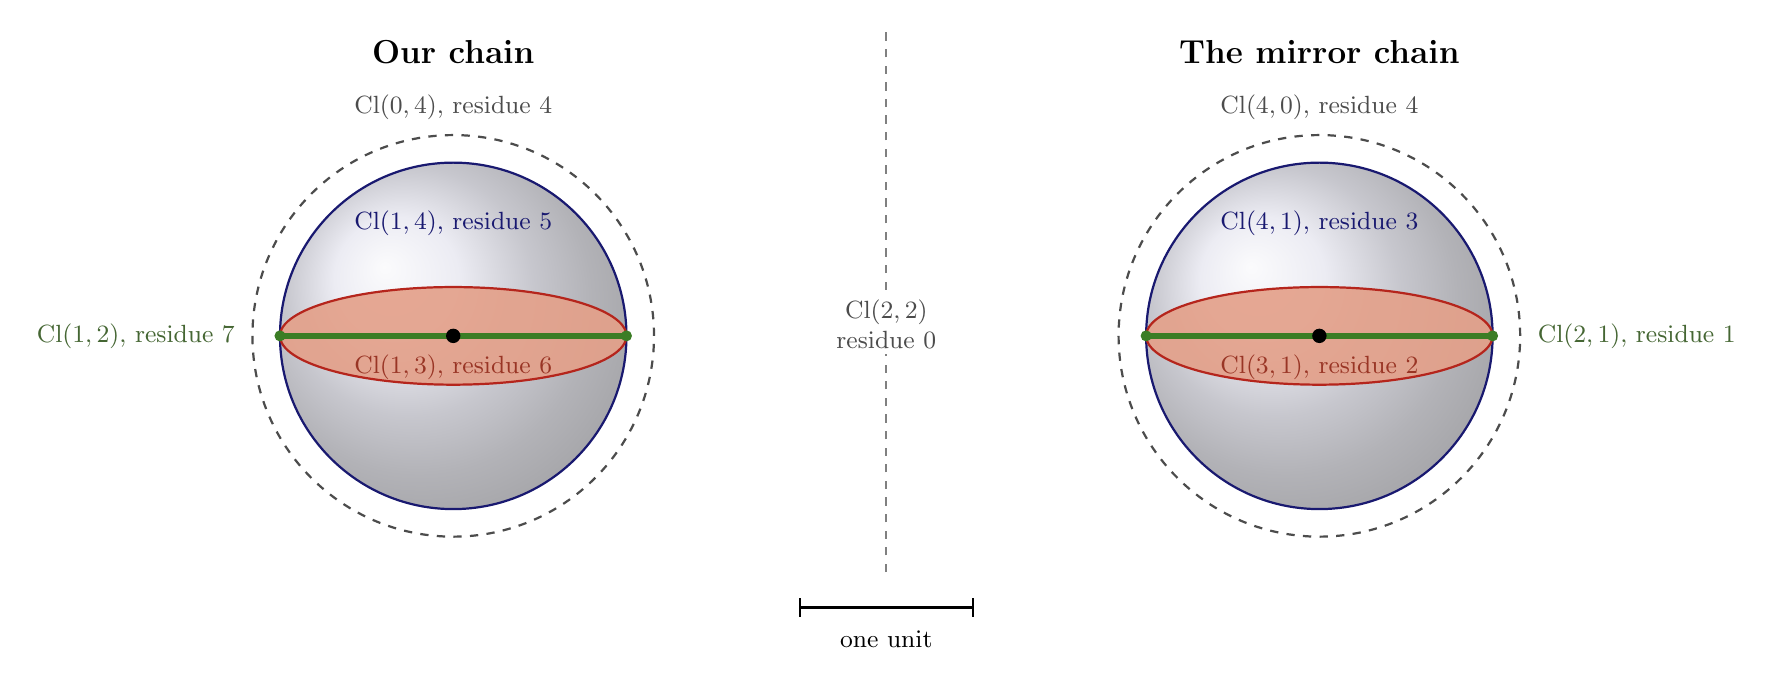
\begin{tikzpicture}[font=\small, >=Stealth]
\newcommand{\chainpic}[5]{%
  \draw[gray!60!black, dashed, thick] (0,0) circle (2.55);
  \shade[ball color=MidnightBlue!22, opacity=0.5] (0,0) circle (2.2);
  \draw[MidnightBlue, thick] (0,0) circle (2.2);
  \fill[BrickRed!35, opacity=0.9] (0,0) ellipse (2.2 and 0.62);
  \draw[BrickRed, thick] (0,0) ellipse (2.2 and 0.62);
  \draw[OliveGreen, line width=2.2pt] (-2.2,0) -- (2.2,0);
  \fill[OliveGreen] (-2.2,0) circle (2pt) (2.2,0) circle (2pt);
  \node[MidnightBlue, font=\small, anchor=south] at (0,1.15) {#1};
  \node[BrickRed!80!black, font=\small, anchor=north] at (0,-0.12) {#2};
  \node[OliveGreen!70!black, font=\small, anchor={\ifnum#5>0 east\else west\fi}] at ({#5*(-2.65)},0) {#3};
  \node[gray!60!black, font=\small, anchor=south] at (0,2.62) {#4};
  \fill[black] (0,0) circle (2.6pt);
}
\begin{scope}
\node[font=\large\bfseries] at (0,3.6) {Our chain};
\chainpic{$\Cl(1,4)$, residue $5$}{$\Cl(1,3)$, residue $6$}{$\Cl(1,2)$, residue $7$}{$\Cl(0,4)$, residue $4$}{1}
\end{scope}
\begin{scope}[xshift=11.0cm]
\node[font=\large\bfseries] at (0,3.6) {The mirror chain};
\chainpic{$\Cl(4,1)$, residue $3$}{$\Cl(3,1)$, residue $2$}{$\Cl(2,1)$, residue $1$}{$\Cl(4,0)$, residue $4$}{-1}
\end{scope}
\draw[gray, dashed, thick] (5.5,-3.0) -- (5.5,3.9);
\node[gray!60!black, font=\small, align=center, fill=white, inner sep=2pt] at (5.5,0.15) {$\Cl(2,2)$\\residue $0$};
\draw[black, thick] (4.4,-3.45) -- (6.6,-3.45);
\draw[black, thick] (4.4,-3.57) -- (4.4,-3.33) (6.6,-3.57) -- (6.6,-3.33);
\node[font=\small, anchor=north] at (5.5,-3.62) {one unit};
\end{tikzpicture}}\\[4pt]
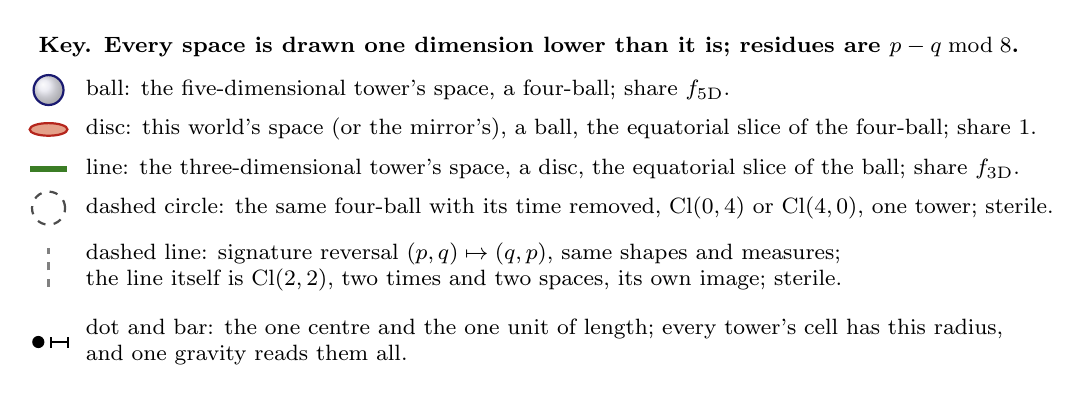
\begin{tikzpicture}[font=\footnotesize]
\node[anchor=west, font=\footnotesize\bfseries] at (0,0.55) {Key. Every space is drawn one dimension lower than it is; residues are $p - q \bmod 8$.};
\shade[ball color=MidnightBlue!22, opacity=0.5] (0.25,0) circle (0.19); \draw[MidnightBlue, thick] (0.25,0) circle (0.19);
\node[anchor=west] at (0.6,0) {ball: the five-dimensional tower's space, a four-ball; share $f_{5\mathrm{D}}$.};
\fill[BrickRed!35] (0.25,-0.5) ellipse (0.24 and 0.08); \draw[BrickRed, thick] (0.25,-0.5) ellipse (0.24 and 0.08);
\node[anchor=west] at (0.6,-0.5) {disc: this world's space (or the mirror's), a ball, the equatorial slice of the four-ball; share $1$.};
\draw[OliveGreen, line width=2pt] (0.02,-1.0) -- (0.48,-1.0);
\node[anchor=west] at (0.6,-1.0) {line: the three-dimensional tower's space, a disc, the equatorial slice of the ball; share $f_{3\mathrm{D}}$.};
\draw[gray!60!black, dashed, thick] (0.25,-1.5) circle (0.21);
\node[anchor=west] at (0.6,-1.5) {dashed circle: the same four-ball with its time removed, $\Cl(0,4)$ or $\Cl(4,0)$, one tower; sterile.};
\draw[gray, dashed, thick] (0.25,-2.5) -- (0.25,-2.0);
\node[anchor=west, align=left] at (0.6,-2.25) {dashed line: signature reversal $(p,q) \mapsto (q,p)$, same shapes and measures;\\the line itself is $\Cl(2,2)$, two times and two spaces, its own image; sterile.};
\fill[black] (0.12,-3.2) circle (2.2pt);
\draw[black, thick] (0.28,-3.2) -- (0.5,-3.2) (0.28,-3.27) -- (0.28,-3.13) (0.5,-3.27) -- (0.5,-3.13);
\node[anchor=west, align=left] at (0.6,-3.2) {dot and bar: the one centre and the one unit of length; every tower's cell has this radius,\\and one gravity reads them all.};
\end{tikzpicture}
\caption{All eight towers as nested spaces. Each world's space is the equatorial slice of the next, and the unit-ball rule compares the volumes of exactly these spaces, $V_{3}/V_{2}$ and $V_{3}/V_{4}$. The two sterile towers are where the picture runs out of time rather than space: residue $4$ is the five-dimensional tower's four-ball with its time removed, residue $0$ has two times and is the dividing line itself.}
\label{fig:geochains}
\end{figure}

\begin{figure}[htbp]\centering
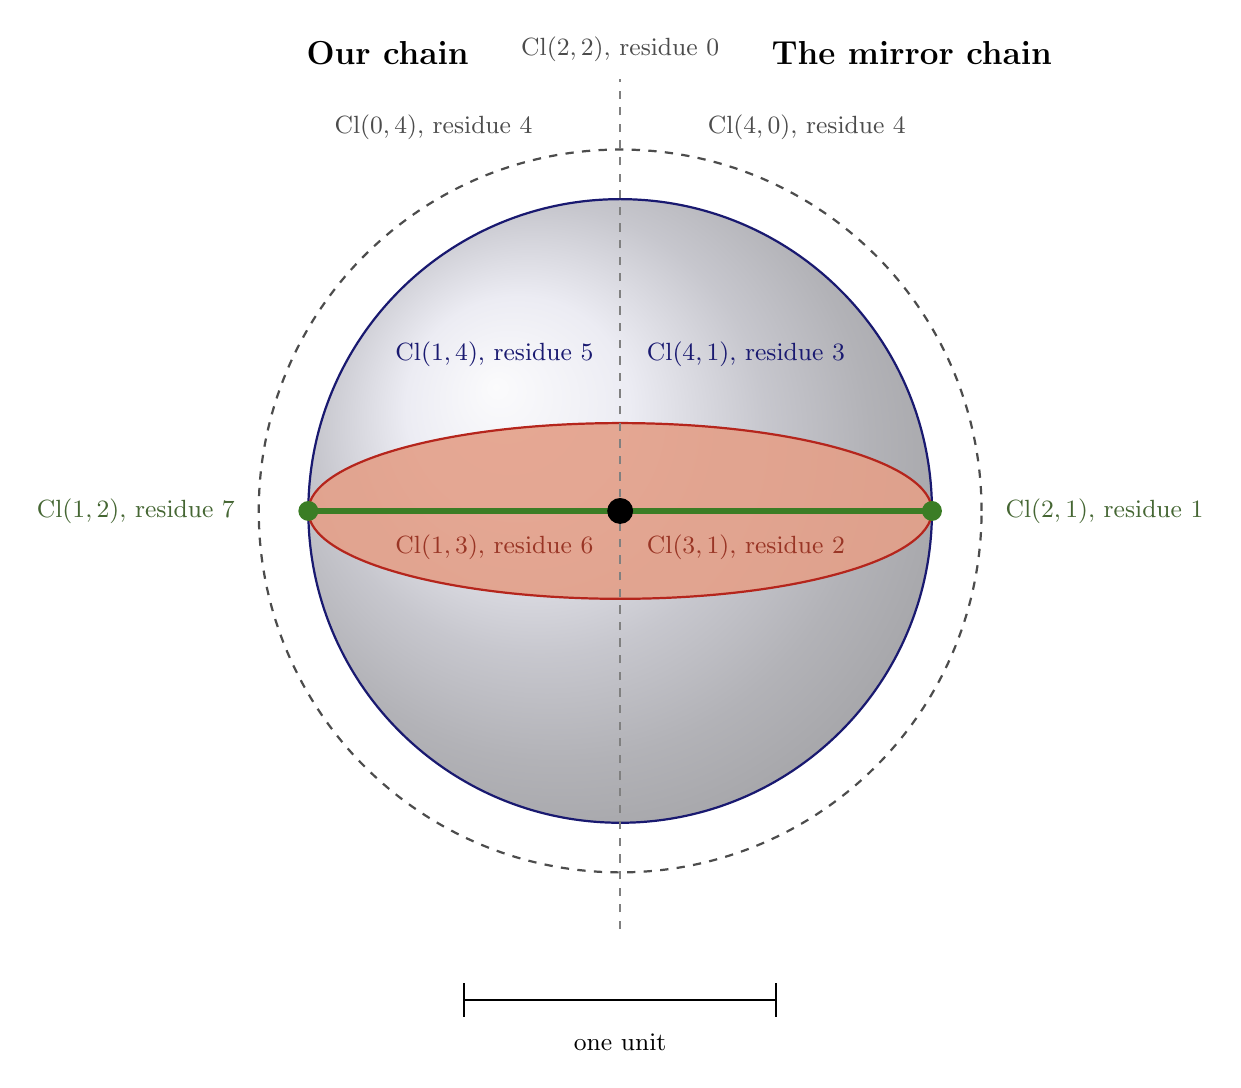
\begin{tikzpicture}[font=\small, >=Stealth, scale=1.8]
\draw[gray!60!black, dashed, thick] (0,0) circle (2.55);
\shade[ball color=MidnightBlue!22, opacity=0.5] (0,0) circle (2.2);
\draw[MidnightBlue, thick] (0,0) circle (2.2);
\fill[BrickRed!35, opacity=0.9] (0,0) ellipse (2.2 and 0.62);
\draw[BrickRed, thick] (0,0) ellipse (2.2 and 0.62);
\draw[OliveGreen, line width=2.2pt] (-2.2,0) -- (2.2,0);
\fill[OliveGreen] (-2.2,0) circle (2pt) (2.2,0) circle (2pt);
\draw[gray, dashed, thick] (0,-2.95) -- (0,3.05);
\fill[black] (0,0) circle (2.6pt);
\node[gray!60!black, font=\small, align=center, anchor=south] at (0,3.1) {$\Cl(2,2)$, residue $0$};
\node[font=\large\bfseries, anchor=south east] at (-1.0,3.08) {Our chain};
\node[font=\large\bfseries, anchor=south west] at (1.0,3.08) {The mirror chain};
\node[MidnightBlue, font=\small, anchor=south east] at (-0.12,0.95) {$\Cl(1,4)$, residue $5$};
\node[MidnightBlue, font=\small, anchor=south west] at (0.12,0.95) {$\Cl(4,1)$, residue $3$};
\node[BrickRed!80!black, font=\small, anchor=north east] at (-0.12,-0.1) {$\Cl(1,3)$, residue $6$};
\node[BrickRed!80!black, font=\small, anchor=north west] at (0.12,-0.1) {$\Cl(3,1)$, residue $2$};
\node[OliveGreen!70!black, font=\small, anchor=east] at (-2.65,0) {$\Cl(1,2)$, residue $7$};
\node[OliveGreen!70!black, font=\small, anchor=west] at (2.65,0) {$\Cl(2,1)$, residue $1$};
\node[gray!60!black, font=\small, anchor=south east] at (-0.55,2.55) {$\Cl(0,4)$, residue $4$};
\node[gray!60!black, font=\small, anchor=south west] at (0.55,2.55) {$\Cl(4,0)$, residue $4$};
\draw[black, thick] (-1.1,-3.45) -- (1.1,-3.45);
\draw[black, thick] (-1.1,-3.57) -- (-1.1,-3.33) (1.1,-3.57) -- (1.1,-3.33);
\node[font=\small, anchor=north] at (0,-3.62) {one unit};
\end{tikzpicture}
\caption{The same eight towers superimposed. Signature reversal is a reflection in the $\Cl(2,2)$ plane, so the mirror chain is the same ball, disc and line read from the other side of it; each tag names the tower on its side, and the dashed circle is one tower named twice. One centre, one unit, one gravity: nothing in the picture belongs to one chain rather than the other except the name, which is what the unit-ball rule assumes when it measures every tower against the same unit ball and the same mass quantum. The symbols are those of Figure \ref{fig:geochains}.}
\label{fig:superpose}
\end{figure}

\begin{proposition}[The nesting]\label{prop:nesting}
Let $H' \subset \R^{4}$ be the hyperplane $x_{4} = 0$.
\begin{enumerate}
\item[(i)] (Algebra.) In $\Cl(1,4)$ the generators $e_{0}, \ldots, e_{3}$ satisfy the relations of $\Cl(1,3)$: this world's algebra is the slice of the residue-$5$ tower's algebra on which the fifth generator is dropped. In $\Cl(1,3)$ the generators $e_{0}, e_{1}, e_{2}$ satisfy those of $\Cl(1,2)$. The mirror chain is the same with the signatures reversed.
\item[(ii)] (Balls of space.) $\B^{4} \cap H' = \B^{3}$ and $\B^{3} \cap \{x_{3} = 0\} = \B^{2}$: our unit ball of space is the equatorial section of the five-dimensional tower's four-ball of space, and the three-dimensional tower's disc of space is the equatorial section of our ball.
\item[(iii)] (Spheres of spacetime.) In $\R^{6} \supset \R^{5} \supset \R^{4}$, $\Sph^{5} \cap \{x_{6} = 0\} = \Sph^{4}$ and $\Sph^{4} \cap \{x_{5} = 0\} = \Sph^{3}$: each world's spacetime sphere is the equator of the next world's. The balls of (ii) carry the space dimension $D$, the spheres of (iii) the spacetime dimension $n = D + 1$, and the hat-box identity of Remark \ref{rem:forms} links the measures of the two.
\end{enumerate}
\end{proposition}

\begin{proof}
(i) The generators square to the diagonal of the smaller signature and anticommute pairwise; the script checks all relations in $\Cl(1,4)$, $\Cl(1,3)$, $\Cl(4,1)$ and $\Cl(3,1)$ with \texttt{GA.py}. (ii) and (iii): a point with one coordinate zero has the same Euclidean norm in the smaller space.
\end{proof}

\begin{figure}[htbp]\centering
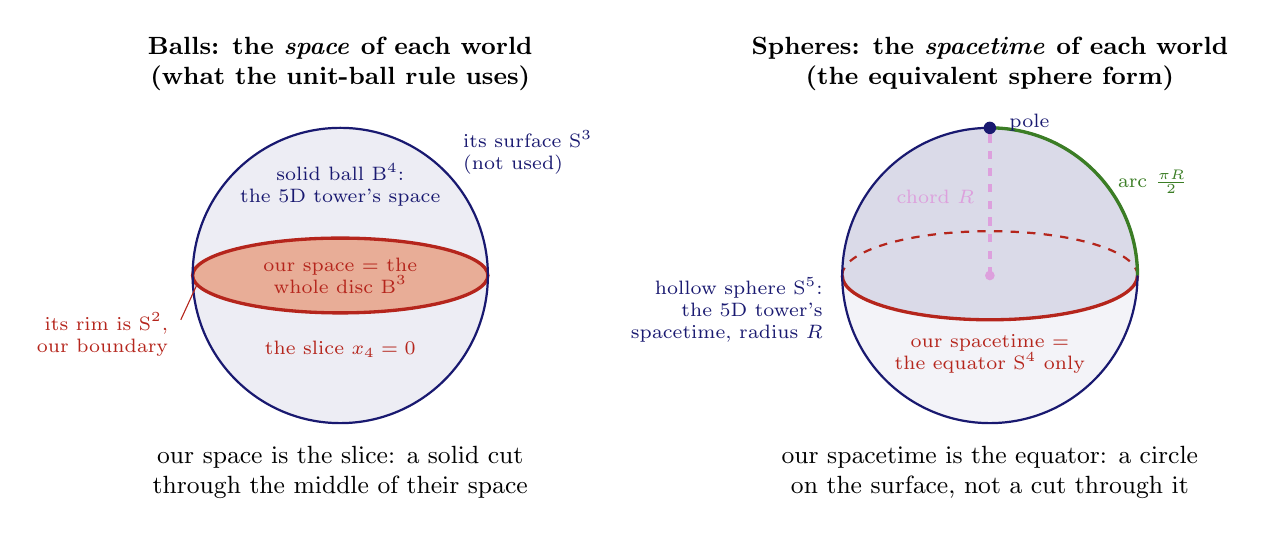
\begin{tikzpicture}[scale=1.25]
\begin{scope}
\fill[MidnightBlue!8] (0,0) circle (1.5);
\fill[BrickRed!30] (0,0) ellipse (1.5 and 0.38);
\draw[BrickRed, very thick] (0,0) ellipse (1.5 and 0.38);
\draw[MidnightBlue, thick] (0,0) circle (1.5);
\node[font=\small\bfseries, align=center] at (0,2.15) {Balls: the \emph{space} of each world\\(what the unit-ball rule uses)};
\node[MidnightBlue, font=\scriptsize, align=center] at (0,0.92) {solid ball $\B^{4}$:\\the 5D tower's space};
\node[MidnightBlue, font=\scriptsize, anchor=west, align=left] at (1.15,1.25) {its surface $\Sph^{3}$\\(not used)};
\node[BrickRed, font=\scriptsize, align=center] at (0,0.0) {our space = the\\whole disc $\B^{3}$};
\node[BrickRed, font=\scriptsize] at (0,-0.75) {the slice $x_{4} = 0$};
\node[BrickRed, font=\scriptsize, align=right, anchor=east] at (-1.65,-0.6) {its rim is $\Sph^{2}$,\\our boundary};
\draw[BrickRed, thin] (-1.62,-0.45) -- (-1.45,-0.08);
\node[font=\small, align=center] at (0,-2.0) {our space is the slice: a solid cut\\through the middle of their space};
\end{scope}
\begin{scope}[xshift=6.6cm]
\node[font=\small\bfseries, align=center] at (0,2.15) {Spheres: the \emph{spacetime} of each world\\(the equivalent sphere form)};
\fill[MidnightBlue!5] (0,0) circle (1.5);
\fill[MidnightBlue!16] (-1.5,0) arc (180:0:1.5) arc (0:-180:1.5 and 0.45) -- cycle;
\draw[BrickRed, dashed, thick] (1.5,0) arc (0:180:1.5 and 0.45);
\draw[BrickRed, very thick] (-1.5,0) arc (180:360:1.5 and 0.45);
\draw[MidnightBlue, thick] (0,0) circle (1.5);
\draw[OliveGreen, very thick] (1.5,0) arc (0:90:1.5);
\draw[Plum, very thick, dashed] (0,0) -- (0,1.5);
\fill[Plum] (0,0) circle (1.4pt);
\fill[MidnightBlue] (0,1.5) circle (1.8pt);
\node[MidnightBlue, font=\scriptsize, anchor=west] at (0.1,1.55) {pole};
\node[MidnightBlue, font=\scriptsize, anchor=east, align=right] at (-1.6,-0.35) {hollow sphere $\Sph^{5}$:\\the 5D tower's\\spacetime, radius $R$};
\node[BrickRed, font=\scriptsize, align=center] at (0,-0.8) {our spacetime =\\the equator $\Sph^{4}$ only};
\node[OliveGreen, font=\scriptsize, anchor=west] at (1.2,0.95) {arc $\tfrac{\pi R}{2}$};
\node[Plum, font=\scriptsize, anchor=east] at (-0.06,0.8) {chord $R$};
\node[font=\small, align=center] at (0,-2.0) {our spacetime is the equator: a circle\\on the surface, not a cut through it};
\end{scope}
\end{tikzpicture}
\caption{The two representations of the nesting. Left, balls of \emph{space} (Proposition \ref{prop:nesting}(ii), two dimensions suppressed): the five-dimensional tower's space is a solid four-ball and our space is the whole disc cut through its middle; the rim of that disc is our own boundary $\Sph^{2}$. This is what the unit-ball rule uses. Right, spheres of \emph{spacetime} (Proposition \ref{prop:nesting}(iii), four dimensions suppressed): the tower's spacetime is a hollow sphere, a surface only, and our spacetime is its equator, a circumference and not a cut. This is the equivalent sphere form of Remark \ref{rem:forms}. On the right, the shaded surface between the equator and one pole has extent $R$ along the polar axis (the chord) and $\tfrac{\pi R}{2}$ along the surface (the arc), the two readings of Proposition \ref{prop:pole}.}
\label{fig:ballsphere}
\end{figure}

\subsection{The rule}\label{subsec:rule}

The rule is stated inside the sourcing rule of Lemma \ref{lem:projection}: the one metric is the four-dimensional one, a tower shares this world's three spatial directions and its time, and the tower's contribution to the metric's source is its energy per unit of the shared three-volume, its content taken homogeneous along every direction it has. Three premises are added. None is supplied by the series.

\begin{premise}[R1: equal mass per quantum]\label{prem:R1}
The quanta of every populated tower carry the same mass $m$.
\end{premise}

\begin{premise}[R2: one quantum per unit ball]\label{prem:R2}
A populated tower whose space has $D$ dimensions ($2$, $3$ or $4$) holds one quantum per unit ball $\B^{D}$ of that space, in one unit of length common to all towers: every tower has the same Wigner-Seitz radius. The rule presupposes that all six towers are populated, which for the odd four is the inference of Observation \ref{obs:population}.
\end{premise}

\begin{premise}[R3: one cell per unshared direction]\label{prem:R3}
In the sourcing rule, a tower's matter counts through exactly one cell radius of each direction its neighbour lacks, on one side: a five-dimensional tower's matter through one radius of its extra direction, and a three-dimensional tower's sheets stacked one radius apart along the direction it lacks. Section \ref{subsec:free} gives a mechanism that returns this value and costs it.
\end{premise}

\begin{remark}[R1 against the series' mass formulas]\label{rem:massR1}
The odd-dimensional mass formulas can be written in a Pfaffian form or in the determinant form of this world's two-constituent formula \cite[Prop.~4.1]{ButlerT11}, and the two are normalised differently; compared across normalisations they make five-dimensional quanta appear at most half as heavy as ours, which would break R1 before it starts. In one normalisation the comparison is even. Let the tower have signature $(1, n-1)$, $n = 3, 4, 5$, with $\gamma^{0}$ Hermitian, $(\gamma^{0})^{2} = 1$, each spatial $\gamma^{k}$ anti-Hermitian, and define $j^{\mu} = \psi^{\dagger}\gamma^{0}\gamma^{\mu}\psi$ and $m^{2} = j_{\mu}j^{\mu}$. Then
\[
m^{2} \;=\; (\psi^{\dagger}\psi)^{2} - \sum_{k}(j^{k})^{2} \;\le\; (\psi^{\dagger}\psi)^{2},
\]
with equality exactly on the eigenvectors of $\gamma^{0}$, where every spatial current vanishes because $\gamma^{k}$ anticommutes with $\gamma^{0}$ and so maps each eigenspace to the other. So the heaviest quantum of unit norm has $m = 1$ in three, four and five dimensions alike (script: the three sets of matrices built exactly, the relations, the bound and its attainment in Gaussian-rational arithmetic). The five-dimensional spinor space is the four-dimensional Dirac space and the first four components of its current are the four-dimensional current, so one five-dimensional constituent is the same object as a four-dimensional Weyl pair, which is why mass begins at one in five dimensions and at two in four: the counts differ, the object does not. This compares the scale of the formulas, not actual masses, which each tower's dynamics sets and the series does not derive. R1 is not in conflict with the series; it is not derived.
\end{remark}

The balls the rule uses. With the standard closed form
\[
V_{D} \;=\; \frac{\pi^{D/2}}{\Gamma\!\left(\frac{D}{2} + 1\right)}, \qquad \Gamma(2) = 1, \quad \Gamma\!\left(\tfrac{5}{2}\right) = \frac{3\sqrt{\pi}}{4}, \quad \Gamma(3) = 2 :
\]
\begin{center}\small
\begin{tabular}{clcccc}
\toprule
$D$ & world & its space & $V_{D}$ & value & $\dfrac{V_{3}}{V_{D}}$ \\[6pt]
\midrule
$2$ & the three-dimensional towers, residues $7$ and $1$ & a disc & $\pi$ & $3.142$ & $\tfrac{4}{3} = 1.3333$ \\[3pt]
$3$ & this world and the mirror, residues $6$ and $2$ & a ball & $\tfrac{4\pi}{3}$ & $4.189$ & $1$ \\[3pt]
$4$ & the five-dimensional towers, residues $5$ and $3$ & a four-ball & $\tfrac{\pi^{2}}{2}$ & $4.935$ & $\tfrac{8}{3\pi} = 0.8488$ \\[3pt]
\bottomrule
\end{tabular}
\end{center}
The share falls with dimension because the unit ball's volume grows from $D = 2$ to $D = 4$ (it peaks at $D = 5$), and one quantum per unit ball is then a lower density.

\begin{proposition}[The unit-ball rule]\label{prop:rule}
Under R1 to R3, the share of a tower whose space has $D$ dimensions is $f = \tfrac{V_{3}}{V_{D}}$, and
\[
\frac{\Omega_{\mathrm{dark}}}{\Omega_{b}} \;=\; V_{3}\sum_{\text{dark }r}\frac{1}{V_{D_{r}}}
\;=\; \frac{V_{3}}{V_{3}} + 2\,\frac{V_{3}}{V_{2}} + 2\,\frac{V_{3}}{V_{4}}
\;=\; 1 + \frac{8}{3} + \frac{16}{3\pi} \;=\; \frac{11\pi + 16}{3\pi} \;=\; 5.36432\ldots
\]
against the observed $5.364 \pm 0.065$.
\end{proposition}

\begin{proof}
By R2 the number density of the tower of residue $r$ in its own space is $1/V_{D_{r}}$ in the common unit, and by R1 its mass density is
\[
\rho_{r} \;=\; \frac{m}{V_{D_{r}}}, \qquad \rho_{\mathrm{us}} \;=\; \frac{m}{V_{3}}.
\]
By R3 that density counts per unit of our three-volume without a further factor: a five-dimensional tower's density per unit four-volume, taken through one unit of the extra direction, is a density per unit three-volume; a three-dimensional tower's density per unit area, with sheets one unit apart, is a density per unit three-volume. Ours is $\rho_{\mathrm{us}}$, the mirror's too. Divide; $m$ cancels. The values are those of the table:
\[
\frac{V_{3}}{V_{2}} \;=\; \frac{4\pi/3}{\pi} \;=\; \frac{4}{3}, \qquad
\frac{V_{3}}{V_{4}} \;=\; \frac{4\pi/3}{\pi^{2}/2} \;=\; \frac{8}{3\pi}, \qquad
1 + 2(1.3333) + 2(0.8488) \;=\; 5.3643 .
\]
The script evaluates the closed form in $(5.36431, 5.36433)$ by rational bounds on $\pi$.
\end{proof}

\begin{remark}[Why the ball is in the denominator]\label{rem:denominator}
The share is a ratio of densities, not of sizes. One quantum per unit ball is a density of $\tfrac{1}{V_{D}}$, so a tower with a larger cell has its one quantum spread over more volume and is filled more thinly: the three-dimensional towers' disc ($3.14$) is smaller than our ball ($4.19$), so their filling is denser and their share exceeds one; the five-dimensional towers' four-ball ($4.93$) is larger, so their filling is sparser and their share is below one. The opposite reading, share proportional to the cell, would say that a larger world holds more matter, which is right for total mass at equal density but is not what gravity in our world sees (Lemma \ref{lem:projection}); it gives $\tfrac{3}{4}$ and $\tfrac{3\pi}{8}$ and a total of $4.856$, excluded at more than seven standard deviations.
\end{remark}

\begin{remark}[What the rule has and has not]\label{rem:rulehas}
One rule is applied identically to every tower, our world entering once, as $V_{3}$, in every comparison, so every share is a multiple of the one $\Omega_{b}$ gravity measures; there is no distinction between towers we contain and towers that contain us, and no observer in another tower would compute a different $\rho_{r}/\rho_{\mathrm{us}}$, because the rule is Lemma \ref{lem:projection} with the thickness R3 states. What the rule does not have is a reason for R1 or R2: R1 is consistent with the series' mass formulas (Remark \ref{rem:massR1}) but not derived; R2 asks every tower to be filled at the same spacing, which for this tower is set by baryon number, a charge the odd towers do not carry (Theorem \ref{thm:paritybit}). R3 is a length, fixed at one cell radius; Section \ref{subsec:free} gives a mechanism that returns that value and costs it. The rule is not the coupling rule of Proposition \ref{prop:norule}: it says nothing about the odd towers' scales, lightest states or number-changing rates, only how much of their matter, whatever it is, sources our metric per unit of our volume.
\end{remark}

\begin{remark}[The extra direction must co-expand]\label{rem:coexpand}
R2 defines one spacing in every direction of each tower's own space, and the spacing grows with the scale factor. If the extra direction were static, a case Lemma \ref{lem:projection} allows, the spacing along it would stay fixed while the spacing along the shared directions grew, so R2 could hold at one epoch only; under the lemma the projected density would still dilute as $a^{-3}$ and the ratio would stay constant, but at a value that is the rule's at one epoch alone. So R2, held at all times, selects the co-expanding case, and today the extra direction is about one baryon spacing, of order a metre comoving, growing with the universe. This is a cost of R2, not of the value R3 gives.
\end{remark}

\begin{remark}[Equivalent forms, and an assignment that is not]\label{rem:forms}
Archimedes' hat-box identity \cite{Archimedes},
\[
|\Sph^{n+1}| \;=\; 2\pi\,V_{n}
\]
(the uniform measure on $\Sph^{n+1}$, projected onto $\R^{n}$ by forgetting two coordinates, is $2\pi$ times the uniform measure on $\B^{n}$; script-checked for $n = 0$ to $6$), gives $|\Sph^{3}| = 2\pi^{2}$, $|\Sph^{4}| = \tfrac{8\pi^{2}}{3}$ and $|\Sph^{5}| = \pi^{3}$. Hence R2 is equivalent to one quantum per unit sphere $\Sph^{n}$, $n = D + 1$, of each tower's spacetime, up to a universal factor $2\pi$ that cancels, and in that form
\[
f_{3\mathrm{D}} = \frac{|\Sph^{4}|}{|\Sph^{3}|} = \frac{4}{3}, \qquad f_{5\mathrm{D}} = \frac{|\Sph^{4}|}{|\Sph^{5}|} = \frac{8}{3\pi}, \qquad
\frac{\Omega_{\mathrm{dark}}}{\Omega_{b}} = |\Sph^{4}|\sum_{\text{dark }r}\frac{1}{|\Sph^{n(r)}|},
\]
with $n(r)$ the tower dimension of residue $r$ and each world's sphere the equator of the next world's (Proposition \ref{prop:nesting}(iii), Figure \ref{fig:ballsphere}). A third assignment, our world as the ball $\B^{4}$ towards a tower we contain and as its boundary $\Sph^{3}$ towards a tower that contains us, $f_{3\mathrm{D}} = \tfrac{V_{3}}{V_{4}}$ and $f_{5\mathrm{D}} = \tfrac{|\Sph^{4}|}{|\Sph^{3}|}$, gives the same two numbers on the opposite towers, and so the same total. It is not physically consistent. Our own density stands in the denominator of every share, and by Lemma \ref{lem:projection} it is one quantity, our mass per unit of our three-volume; this assignment reads our world as a volume in one comparison and as a surface in the other, and so gives our own density two values at once, which one metric cannot see. It is not a mechanism, since no rule can count our own density two ways (script: no fixed divisor with unit regions reproduces that pair in that order), and Proposition \ref{prop:Tc} shows it is the family at thickness $\tfrac{\pi}{2}$, the arc of Proposition \ref{prop:pole} in place of the flat chord that R2's cells have. So the ball and sphere forms are one rule, the factor $2\pi$ cancelling, while the exchanged assignment agrees with them in the total only. The two differ in composition: under the rule dark matter is $18.6\%$ mirror, $49.7\%$ three-dimensional and $31.6\%$ five-dimensional, and under the exchanged assignment the last two are exchanged. The total cannot tell them apart, and that difference is what the galaxy-cluster tests of Section \ref{subsec:simulated} probe. Read at composite strength (Proposition \ref{prop:audit}), the colliding share of the dark matter, the mirror's included, is $68\%$ under the rule and $50\%$ under the exchanged assignment, and both fail the Bullet Cluster and the shapes of galaxy clusters. With the odd towers' matter collisionless both collide only the mirror's $18.6\%$, and those tests cannot separate them. Either way the choice between the two rests on the consistency argument above, not on the clusters.
\end{remark}

\subsection{The thickness: a contact mechanism}\label{subsec:free}

R3 is a premise: it fixes the thickness at one cell radius, on one side, and nothing in the series does. This subsection gives a mechanism that returns that value. The count is made in the towers' own spaces, by asking which quanta of a tower are in contact with a world whose space is a slice of the tower's, the count being made on the nested world's space and carried to the containing world's by reciprocity. The mechanism has four clauses on how cells make contact. They were chosen with the value known, each has a stated alternative that the observation excludes (Table \ref{tab:excludes}), and the mechanism holds for one nesting at a time and does not compose across two (Remark \ref{rem:scope}). So what follows explains R3's value and does not derive it, and the tier of the rule is unchanged. The one-parameter family in which the thickness is a parameter is recorded afterwards as the sensitivity analysis. Throughout, $d_{b}$ is the common spacing of R2, the Wigner-Seitz radius, lengths are in units of it, a quantum's \emph{cell} is the ball of radius one about it in its tower's space, and a count is \emph{downward} when a world counts the cells of the tower whose space contains its own.

\emph{The four clauses.} (C) Contact: a quantum sources a world whose space is a slice of its tower's exactly when its cell meets that slice. (I) Indivisibility: a quantum that sources a world counts whole, its mass $m$ and not a fraction of it set by how much of its cell the slice cuts. (S) The side: across the direction a nesting adds or lacks, sourcing runs on one side only, the side named by the sign of the central volume element $\omega$ of the odd member of the nesting, whether that member is the tower counted or the world counting; where the odd member has two modules (residues $1$ and $5$) each module names a side, and a sheet of the three-dimensional tower holds one module. (O) Reciprocity: the ratio of two nested towers' densities found by the downward count on the nested world's space is the ratio read on the containing world's space. S postulates the side; Lemma \ref{lem:fifth} only says what a side is. O is the equality of R3's two thicknesses in another form (Proposition \ref{prop:thickness}(iii)).

\begin{lemma}[The direction a nesting adds, in the algebra]\label{lem:fifth}
Write $P$ for the even world's pseudoscalar, the ordered product of its generators, and $\omega$ for the central volume element of the odd tower. In the four nestings of Proposition \ref{prop:nesting}(i):
\begin{enumerate}
\item[(i)] (Residue $5$, $\Cl(1,4) \supset \Cl(1,3)$.) $\omega = e_{0}e_{1}e_{2}e_{3}e_{4}$ is central with $\omega^{2} = +1$, $P = e_{0}e_{1}e_{2}e_{3}$ has $P^{2} = -1$, and the fifth direction is
\[
e_{4} \;=\; P^{-1}\omega .
\]
Reversing our orientation, $P \mapsto -P$ with $\omega$ fixed, reverses $e_{4}$. The central idempotents $\tfrac{1}{2}(1 \pm \omega)$ cut out the two simple components on which the two irreducible modules live (Theorem \ref{thm:types}(iv)), and $e_{4}$ acts on them as $\pm P^{-1}$. The reflection through our world, $x_{4} \mapsto -x_{4}$, fixes $P$ and sends $\omega \mapsto -\omega$: it exchanges the two components.
\item[(ii)] (Residue $3$, $\Cl(4,1) \supset \Cl(3,1)$.) The mirror's algebra is the slice $\{e_{0}, e_{1}, e_{2}, e_{4}\}$ with $P = e_{0}e_{1}e_{2}e_{4}$, $P^{2} = -1$; $\omega^{2} = -1$, one module; the added direction is $e_{3} = -P^{-1}\omega$, reversed by $P \mapsto -P$.
\item[(iii)] (Residue $7$, $\Cl(1,2) \subset \Cl(1,3)$.) $\omega = e_{0}e_{1}e_{2}$ is central in the slice with $\omega^{2} = -1$, and the direction the three-dimensional tower lacks is $e_{3} = \omega^{-1}P$.
\item[(iv)] (Residue $1$, $\Cl(2,1) \subset \Cl(3,1)$.) The slice is $\{e_{0}, e_{1}, e_{3}\}$, $\omega = e_{0}e_{1}e_{3}$ is central in it with $\omega^{2} = +1$, two modules, and the lacking direction is $e_{2} = -\omega^{-1}P$.
\end{enumerate}
These are identities: $\omega$ is the ordered product $P e_{4}$ (or $\omega_{3}e_{3}$), so each equation restates the ordering, and its sign under $P \mapsto -P$ is immediate. What they fix is the meaning of a side: given the even world's orientation, the sign of $\omega$ is the sign of the direction the nesting adds or removes. Where $\omega^{2} = +1$ (residues $5$ and $1$) that sign is a label a quantum carries, its simple component; where $\omega^{2} = -1$ (residues $3$ and $7$) $-\omega$ is the conjugate complex structure on the same real module, and the sign is a convention for the tower as a whole. The lemma supplies no half-space: that a quantum sources on the side its sign names is clause S.
\end{lemma}

\begin{proof}
Direct computation in each slice, the minus signs in (ii) and (iv) coming from moving one generator past another; $e_{4}\cdot\tfrac{1}{2}(1 \pm \omega) = \pm P^{-1}\cdot\tfrac{1}{2}(1 \pm \omega)$ since $\omega(1 \pm \omega) = \pm(1 \pm \omega)$; the reflection $v \mapsto -e_{4}ve_{4}^{-1}$ fixes $e_{0}$ to $e_{3}$ and negates $e_{4}$. Centrality and the squares of $\omega$ are the centre computation in the proof of Theorem \ref{thm:types}. The script computes all of it in \texttt{GA.py}.
\end{proof}

\begin{proposition}[The contact mechanism returns R3]\label{prop:thickness}
Under R1, R2 and the clauses C, I, S and O:
\begin{enumerate}
\item[(i)] a five-dimensional tower's matter sources this world through exactly one cell radius of its extra direction, so $f_{5\mathrm{D}} = \tfrac{V_{3}}{V_{4}}$;
\item[(ii)] a three-dimensional tower's sheets are one cell radius apart, so $f_{3\mathrm{D}} = \tfrac{V_{3}}{V_{2}}$;
\item[(iii)] hence the mechanism returns R3: its unit is the cell radius R2 chose, its one side is S, which supplies a factor one half against the two-sided count, and the equality of its two thicknesses is O. The spacing $d_{b}$ cancels and the total is Proposition \ref{prop:rule}'s.
\end{enumerate}
\end{proposition}

\begin{proof}
(i) Take coordinates on the five-dimensional tower's space $\R^{4}$ with our space the hyperplane $x_{4} = 0$ (Proposition \ref{prop:nesting}(ii)). By R2 the quanta's centres have density $1/V_{4}$ per unit four-volume. A cell, the unit ball about a centre at height $x_{4} = h$, meets the hyperplane exactly when $|h| \leq 1$ (C); each such quantum counts whole (I); and each sources on one side only (S), the side its sign of $\omega$ names through Lemma \ref{lem:fifth}(i). Which side is immaterial to the number: the quanta of one sign source our world from the slab $0 \leq h \leq 1$ and those of the other from $-1 \leq h \leq 0$, and whether the tower holds both signs at half the density each or one sign at the whole density, the quanta sourcing our world per unit of our three-volume number
\[
\int_{0}^{1}\frac{dh}{V_{4}} \;=\; \frac{1}{V_{4}},
\]
one cell radius of the extra direction; with R1 the density is $m/V_{4}$ against ours, $m/V_{3}$.

(ii) The contact count runs downward only. A cell of the containing tower is a solid region meeting the nested world's space in a region of positive measure, whereas the cells of a tower nested in this world are discs in a sheet, and no count of discs per unit of our three-volume is defined until the sheets' spacing is. So count on the three-dimensional tower's own space, the plane $x_{3} = 0$ in ours (Proposition \ref{prop:nesting}(ii)), where our quanta are the containing tower's: their centres have density $1/V_{3}$ per unit three-volume, a cell meets the plane when $|x_{3}| \leq 1$, it counts whole, and each sheet is sourced from one side, the side named by the sheet's own $\omega$ across the direction it lacks (Lemma \ref{lem:fifth}(iii) or (iv); at residue $1$ each module names a side, and S takes each sheet to hold one module, so a sheet of either kind is sourced from one side; a sheet holding both would be sourced from both, at $2/V_{3}$). Per unit area of the plane our quanta number $1/V_{3}$ and the tower's own $1/V_{2}$, so on that world
\[
\frac{\rho_{\mathrm{us}}}{\rho_{3\mathrm{D}}} \;=\; \frac{V_{2}}{V_{3}} .
\]
By O the same ratio holds read on our space, $\rho_{3\mathrm{D}}/\rho_{\mathrm{us}} = V_{3}/V_{2}$. A family of sheets $s$ apart, each of density $m/V_{2}$ per unit area, has density $m/(V_{2}s)$ per unit three-volume, so $s = 1$: the sheets are one cell radius apart, which is the sheet clause of Lemma \ref{lem:projection} with its unit named. The nestings over the mirror (residues $3$ and $1$) are not reached by the count, since the residue-$3$ tower's space contains the mirror's and not ours; $f_{3} = f_{5}$ and $f_{1} = f_{7}$ are P2's audit along the reversal orbit, as in \eqref{eq:sum}.

(iii) (i) and (ii) are R3's two clauses with the value one cell radius. The unit is R2's: with any other cell convention the contact slab has another width (the mean spacing is $n^{-1/3} = 1.61\,d_{b}$, and cubic cells give the $5.000$ of Table \ref{tab:costs}). Two-sided contact gives $2/V_{4}$, so S is the factor one half. In (ii) the downward count fixes $\rho_{\mathrm{us}}/\rho_{3\mathrm{D}}$ on the sheet, and for sheets $s$ apart the ratio read on our space is $V_{3}/(sV_{2})$; O sets the two equal, which is $s = 1$, so O is the equality of the sheet spacing and the extra length. Every count is a number of quanta per unit region of radius $d_{b}$, so $d_{b}$ cancels in each ratio as $m$ does by R1. The script recomputes the slab count as an integral, the downward count, the total, the alternatives of Table \ref{tab:excludes}, and the non-composition of Remark \ref{rem:scope}.
\end{proof}

\begin{table}[htbp]\centering\small
\begin{tabular}{lcccc}
\toprule
Clause withdrawn & $f_{5\mathrm{D}}$ & $f_{3\mathrm{D}}$ & total & against $5.364 \pm 0.065$ \\
\midrule
none (the mechanism) & $\tfrac{8}{3\pi}$ & $\tfrac{4}{3}$ & $5.364$ & $0\sigma$ \\[2pt]
S: both sides count & $\tfrac{16}{3\pi}$ & $\tfrac{2}{3}$ & $5.729$ & $5.6\sigma$ high \\[2pt]
I: a cut cell counts by its section, one side & $\tfrac{1}{2}$ & $2$ & $6.000$ & $9.8\sigma$ high \\[2pt]
I and S: by section, both sides & $1$ & $1$ & $5.000$ & $5.6\sigma$ low \\[2pt]
O: the sheet spacing is not the extra length & $\tfrac{8}{3\pi}$ & free & $1 + \tfrac{16}{3\pi} + 2f_{3\mathrm{D}}$ & $c_{3} \in [0.976, 1.025]$ \\[2pt]
C: the homogeneous integral of Lemma \ref{lem:projection} & $\tfrac{8c}{3\pi}$ & $\tfrac{4}{3c}$ & $T(c)$ & the family below \\
\bottomrule
\end{tabular}
\caption{The mechanism's four clauses and the nearest alternative to each. The section weighting counts a cut cell by the measure of its section relative to the maximal section, one normalisation among several: a unit $D$-ball cut at height $h$ has section measure $V_{D-1}(1 - h^{2})^{(D-1)/2}$, and relative to $V_{D-1}$ these weights integrate over both sides to $V_{D}/V_{D-1}$, which for $D = 4$ is $\tfrac{3\pi}{8}$, the $\cos^{4}$ factor of the zero-mode reduction (Proposition \ref{prop:reduction}(i)); that reduction is the five-dimensional count with I and S withdrawn. With C withdrawn the sourcing rule reverts to the homogeneous integral over a length $c$, which is Proposition \ref{prop:Tc}. The list is the paper's, not exhaustive; other cell conventions and other normalisations of a partial count are not on it.}
\label{tab:excludes}
\end{table}

\begin{remark}[What S uses, and what it does not]\label{rem:Sfork}
S needs a side for each sourcing quantum or sheet, and the side is postulated. What the lemma supplies is that a side exists: in an odd tower $\omega$ is central, so its sign is a label a quantum carries where the centre splits and a convention for the tower where it does not, and in the even neighbour's frame that sign is the sign of the direction the nesting adds; the even towers have no such sign, their centre being $\R$. S selects no module: where $\omega^{2} = +1$, Theorem \ref{thm:modes}(ii) counts both modules under P2, R2 with S then puts each at half the density on its own side, and the two slabs sum to one cell radius, exactly as if one module held the whole density. Where $\omega^{2} = -1$ the sign is a convention for the tower, every quantum sources the same side, and the count is one cell radius at full density. S uses no orientation off the reversal orbit: reversing the neighbour's $P$ exchanges every side at once and the count is unchanged, so P1's orientation clause stays where Premise \ref{prem:single} keeps it. And S does not orient the odd tower's family: Theorem \ref{thm:paritybit} concerns the flag bit, and the sign of $\omega$ is a different object. What is postulated is the one-sidedness itself, and for the residue-$1$ sheets the further stipulation that a sheet holds one module; without the first both sides count and the total is $5.729$ (Table \ref{tab:excludes}), and without the second the residue-$1$ sheets are sourced from both sides.
\end{remark}

\begin{remark}[Scope of the mechanism]\label{rem:scope}
Two limits keep the mechanism an explanation of R3's value rather than a derivation of it. First, it does not compose. For the double nesting of the three-dimensional tower's plane in the five-dimensional tower's space, R3 gives $\rho_{5\mathrm{D}}/\rho_{3\mathrm{D}} = V_{2}/V_{4} = 0.637$, one cell radius for each of the two unshared directions; counting the five-dimensional cells that meet the plane directly by C and I gives $V_{2}^{2}/V_{4} = 2$ on the full transverse disc, $1$ on a half-disc and $\tfrac{1}{2}$ on a quadrant, and S is undefined there, $P^{-1}\omega$ across two directions being a bivector. So C with I holds for adjacent nestings only, which is where the rule uses it, and O is not tested there; R3, which composes, is the statement, and the mechanism is a reading of one step. Second, C restricts the homogeneous integral of Lemma \ref{lem:projection} to one cell radius, and under it the five-dimensional tower's matter further from this world sources the one metric not at all. With P1 that matter is either absent, so that the extra direction is about one cell deep (the co-expanding direction of Remark \ref{rem:coexpand}, forced rather than allowed) and C adds nothing to the integral over it, which is R3; or present and inert to gravity, against Proposition \ref{prop:sourcing}(i), which takes the integral over the whole direction as the only covariant choice. On the first branch C is R3; on the second it contradicts a proposition the paper calls forced. On neither is it a foundation.
\end{remark}

\paragraph*{Sensitivity.} The rest of this subsection records the total's dependence on the thickness taken as a parameter, which is where the observation's constraint on R3 lives.

\begin{proposition}[The total as a function of the thickness]\label{prop:Tc}
Let the five-dimensional towers' matter count through a length $c\,d_{b}$ of the extra direction and the three-dimensional towers' sheets be stacked $c\,d_{b}$ apart, with R1, R2 and the sourcing rule otherwise as before. Then
\[
T(c) \;:=\; \frac{\Omega_{\mathrm{dark}}}{\Omega_{b}} \;=\; 1 + \frac{8}{3c} + \frac{16c}{3\pi},
\]
and:
\begin{enumerate}
\item[(i)] $T(c) = T\!\left(\dfrac{\pi}{2c}\right)$ for every $c > 0$;
\item[(ii)] $T$ has a single minimum,
\[
c_{\ast} = \sqrt{\frac{\pi}{2}} = 1.2533, \qquad T_{\ast} = 1 + 2\sqrt{\frac{128}{9\pi}} = 5.2554,
\]
which is $1.7\sigma$ below the observed value; no thickness gives less;
\item[(iii)] $T(c) = 5.3643$ exactly at $c = 1$ and $c = \tfrac{\pi}{2}$, the two roots of one quadratic, with product $\tfrac{\pi}{2}$;
\item[(iv)] against $5.364 \pm 0.065$ the allowed thicknesses are $c \in [0.943, 1.086]$ or $c \in [1.447, 1.667]$ at one standard deviation, and the single interval $c \in [0.898, 1.750]$ at two;
\item[(v)] the three-dimensional fraction of dark matter, which self-interacts if that matter is at composite strength (Proposition \ref{prop:audit}), is
\[
\frac{2 f_{3\mathrm{D}}}{T(c)} \;=\; \frac{8}{3c\,T(c)} : \qquad 49.7\% \text{ at } c = 1, \quad 40.5\% \text{ at } c_{\ast}, \quad 31.6\% \text{ at } c = \tfrac{\pi}{2}.
\]
\end{enumerate}
\end{proposition}

\begin{proof}
Per unit of our three-volume the three densities are
\[
\rho_{5\mathrm{D}} = \frac{m\,c}{V_{4}\,d_{b}^{3}}, \qquad
\rho_{3\mathrm{D}} = \frac{m}{c\,V_{2}\,d_{b}^{3}}, \qquad
\rho_{\mathrm{us}} = \frac{m}{V_{3}\,d_{b}^{3}},
\]
so the shares are
\[
f_{3\mathrm{D}} = \frac{V_{3}}{c\,V_{2}} = \frac{4}{3c}, \qquad f_{5\mathrm{D}} = \frac{c\,V_{3}}{V_{4}} = \frac{8c}{3\pi},
\]
and the sum is \eqref{eq:sum}. (i) Substitute. (ii) $T$ is of the form $1 + \frac{A}{c} + Bc$ with $A = \frac{8}{3}$ and $B = \frac{16}{3\pi}$; by the arithmetic-geometric inequality
\[
\frac{A}{c} + Bc \;\geq\; 2\sqrt{AB}, \qquad \text{with equality at } c = \sqrt{\frac{A}{B}} = \sqrt{\frac{\pi}{2}} .
\]
(iii) $T(c) = T(1)$ is the quadratic
\[
Bc^{2} - \bigl(T(1) - 1\bigr)c + A = 0, \qquad c_{1}c_{2} = \frac{A}{B} = \frac{\pi}{2};
\]
$c = 1$ is a root by construction and $\frac{\pi}{2}$ is the other. (iv) and (v) are evaluation. The script checks (i) as an identity in $\pi$ for rational $c$, brackets $T_{\ast}$ and the window endpoints by rational bounds on $\pi$ and on the square root, and evaluates the fractions.
\end{proof}

\begin{figure}[htbp]\centering
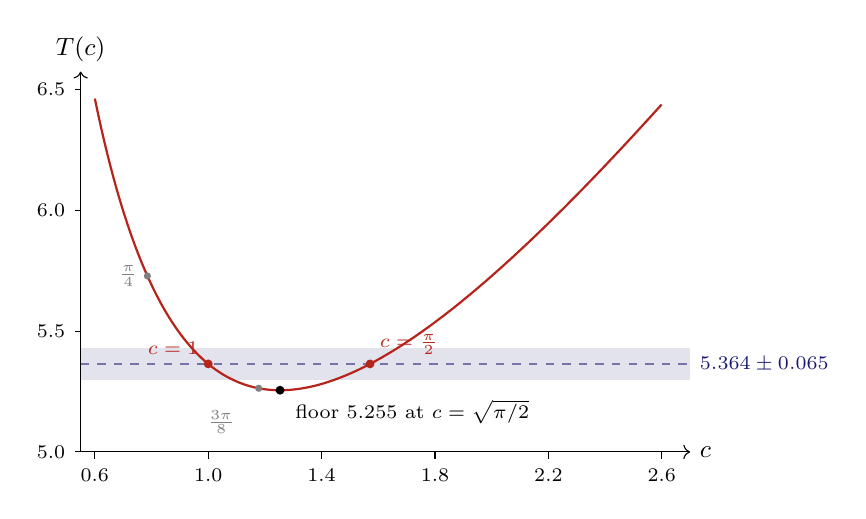
\begin{tikzpicture}[x=3.6cm, y=4.6cm]
\draw[->] (0.55,0) -- (2.7,0) node[right, font=\small] {$c$};
\draw[->] (0.55,0) -- (0.55,1.05) node[above, font=\small] {$T(c)$};
\foreach \x in {0.6,1.0,1.4,1.8,2.2,2.6} { \draw (\x,0) -- (\x,-0.02) node[below, font=\scriptsize] {\x}; }
\foreach \y/\lab in {0/5.0,0.3333/5.5,0.6667/6.0,1.0/6.5} { \draw (0.55,\y) -- (0.53,\y) node[left, font=\scriptsize] {\lab}; }
\fill[MidnightBlue!12] (0.55,0.1993) rectangle (2.7,0.2860);
\draw[MidnightBlue!60, dashed] (0.55,0.2427) -- (2.7,0.2427) node[right, font=\scriptsize, MidnightBlue] {$5.364 \pm 0.065$};
\draw[BrickRed, thick, domain=0.6:2.6, samples=120, smooth] plot (\x, {(1 + 8/(3*\x) + 16*\x/(3*pi) - 5)/1.5});
\fill[BrickRed] (1,0.2429) circle (1.6pt) node[above left, font=\scriptsize] {$c = 1$};
\fill[BrickRed] (1.5708,0.2429) circle (1.6pt) node[above right, font=\scriptsize] {$c = \tfrac{\pi}{2}$};
\fill[black] (1.2533,0.1703) circle (1.6pt) node[below right, font=\scriptsize, xshift=2pt] {floor $5.255$ at $c = \sqrt{\pi/2}$};
\fill[gray] (1.1781,0.1757) circle (1.3pt);
\node[gray, font=\scriptsize, anchor=north east] at (1.13,0.14) {$\tfrac{3\pi}{8}$};
\fill[gray] (0.7854,0.4857) circle (1.3pt) node[left, gray, font=\scriptsize] {$\tfrac{\pi}{4}$};
\end{tikzpicture}
\caption{The total $T(c) = 1 + \tfrac{8}{3c} + \tfrac{16c}{3\pi}$ against the thickness $c$ in units of the spacing (Proposition \ref{prop:Tc}), with the Planck-with-lensing band. The curve is symmetric under $c \mapsto \tfrac{\pi}{2c}$ and has its floor at $c = \sqrt{\pi/2}$. The observed value is met at $c = 1$ (R3) and at $c = \tfrac{\pi}{2}$ (the exchanged assignment of Remark \ref{rem:forms}). The grey points are the two thicknesses the de Sitter reductions of Section \ref{subsec:unit} produce, $\tfrac{3\pi}{8}$ and $\tfrac{\pi}{4}$; neither is on the band.}
\label{fig:Tc}
\end{figure}

\begin{proposition}[The two roots are the chord and the arc of a quarter turn]\label{prop:pole}
In the sphere form of the rule, represent the five-dimensional tower's spacetime by a sphere of radius $R$ with our spacetime as its equator. The region between the equator and one pole has extent $R$ along the polar axis (the chord) and $\tfrac{\pi R}{2}$ along the surface (the arc). With $R = d_{b}$: counting the tower's matter per unit chord over that region is the unit-ball rule, $c = 1$; counting it per unit arc is the exchanged assignment, $c = \tfrac{\pi}{2}$; and the two totals agree because Proposition \ref{prop:Tc}(i) exchanges them, while their compositions differ (Remark \ref{rem:forms}). R2 selects the chord: its cells are unit balls of the tower's flat space, whose measure along the added direction is the radius. Between the equator and both poles the values are $c = 2$ and $c = \pi$, giving $5.729$ and $7.182$, both excluded.
\end{proposition}

\begin{proof}
The chord from the equatorial plane to a pole is the radius; the arc is a quarter of a great circle. With both poles,
\[
T(2) = 1 + \frac{4}{3} + \frac{32}{3\pi} = 5.729, \qquad T(\pi) = 1 + \frac{8}{3\pi} + \frac{16}{3} = 7.182 ;
\]
the script brackets both and confirms that each misses by more than four standard deviations. The clock reflection $r \mapsto 4 - r$, which exchanges each three-dimensional tower with a five-dimensional one, is the bookkeeping image of (i) and not a symmetry of the physics, the two odd types differing in gauge content and algebra type.
\end{proof}

\begin{remark}[The common thickness, and the curve if the two differ]\label{rem:twoc}
R3 takes the extra length and the sheet spacing equal; in the mechanism that equality is clause O. Let them differ, $c_{5}$ and $c_{3}$. With $c_{5} = 1$ kept, the observation confines $c_{3}$ to $[0.976, 1.025]$ at one standard deviation and nothing else constrains it; with both free it fixes a curve,
\[
\frac{8}{3c_{3}} + \frac{16c_{5}}{3\pi} \;=\; 4.364,
\]
whose two intersections with the diagonal $c_{3} = c_{5}$ are the roots of Proposition \ref{prop:Tc}(iii), and off the diagonal nothing natural lands on it ($c_{3} = \tfrac{4}{3}$ needs $c_{5} = 1.39$, $c_{3} = 2$ needs $c_{5} = 1.79$).
\end{remark}

\subsection{What could fix the unit: the de Sitter reading}\label{subsec:unit}

The rule needs one length common to all towers. The series fixes exactly one length, and this subsection follows it.

\begin{fact}[imported: the frozen point and the de Sitter radius]\label{fact:dsradius}
On the Einstein region with $\Lambda > 0$ the parallel scale tractor $I$ has squared norm $\ip{I}{I} = \tfrac{\Lambda}{3}$, its stabiliser is the de Sitter group $SO(1,4)$, its orthogonal complement $I^{\perp}$ carries the induced form of signature $(1,4)$, and the flat-model section is the de Sitter hyperboloid of radius $\ell$, $\ell^{2} = \tfrac{3}{\Lambda}$. Under the action as written, $\Lambda$ is a parameter of the laws, not initial data. \emph{Provenance:} \cite[Thm.~4.7, Prop.~4.10, Prop.~4.4]{ButlerT6}; \cite[Fact~2.1, Thm.~3.1, Prop.~5.8]{ButlerT10}.
\end{fact}

By Fact \ref{fact:dsradius}, our world with $\Lambda > 0$ is de Sitter space of radius $\ell = \sqrt{\tfrac{3}{\Lambda}}$ at the level of the frozen point, and Euclidean de Sitter space $\dS_{4}$ is $\Sph^{4}$ of radius $\ell$, the boundary of $\B^{5}$ of radius $\ell$. The towers share one gravity, and $\Lambda$ is a parameter of the laws, so every tower has the same $\Lambda$ and its own Euclidean de Sitter sphere $\Sph^{n(r)}$ of the same radius $\ell$; the nesting of Proposition \ref{prop:nesting}(iii) is the nesting of these spheres by equators. So the objects of the rule's sphere form (Remark \ref{rem:forms}), and the common unit R2 needs, are already in the series, with the unit the de Sitter radius rather than a microscopic spacing.

\begin{premise}[D: democracy of the total mass]\label{prem:D}
Every populated tower carries the same total mass $M_{\mathrm{tot}}$ on its de Sitter sphere. This is a democracy of mass, distinct from P4's democracy of the asymmetry, which the odd towers do not carry.
\end{premise}

\begin{proposition}[Democracy at the de Sitter radius is the unit-ball rule]\label{prop:democracy}
Under D, with the thickness set to $\ell$ (R3 with $\ell$ as the unit), the shares are $\tfrac{|\Sph^{4}|}{|\Sph^{n}|}$, the sphere form of Remark \ref{rem:forms}, and the total is that of Proposition \ref{prop:rule}.
\end{proposition}

\begin{proof}
A tower of dimension $n$ has density $\frac{M_{\mathrm{tot}}}{|\Sph^{n}|\,\ell^{n}}$ on its sphere; through a thickness $\ell$ of the direction we cannot see, or with sheets $\ell$ apart, that becomes a density per unit of our four-measure, and the share is
\[
f \;=\; \frac{M_{\mathrm{tot}}}{|\Sph^{n}|\,\ell^{4}} \Bigg/ \frac{M_{\mathrm{tot}}}{|\Sph^{4}|\,\ell^{4}} \;=\; \frac{|\Sph^{4}|}{|\Sph^{n}|} . \qedhere
\]
\end{proof}

This reading removes the two costs Remarks \ref{rem:rulehas} and \ref{rem:coexpand} record: no conserved count is needed to fill the odd towers at one microscopic spacing, and there is no metre-scale expanding extra dimension. Two things stand against it. First, under the sourcing rule a five-dimensional tower's fifth direction is a direction of its own space, not of spacetime, so the residue-$5$ tower cannot be identified with our own tractor ambient $I^{\perp}$; the reading survives only as ``each tower has its own $\dS_{n}$ at the shared $\Lambda$'', which the series permits and does not make. Second, the thickness is still R3's, now at one de Sitter radius: within the series as written there is no $\dS_{5}$ to slice, because there is no five-dimensional Einstein equation for it to solve, and $c$ is exactly the freedom P1 leaves, which R3 fixes, the contact mechanism of Section \ref{subsec:free} explains, and the geometry does not reach. To compute the thickness at all one must promote the fifth direction to a metric direction, against the sourcing rule. Doing so: $\dS_{5}$ of radius $\ell$ is foliated by $\dS_{4}$ slices,
\begin{equation}\label{eq:warp}
ds_{5}^{2} = \ell^{2}d\theta^{2} + \cos^{2}\theta\; ds_{4}^{2}, \qquad \theta \in (-\pi/2, \pi/2),
\end{equation}
with our world the equator $\theta = 0$. Let the five-dimensional tower's dust fill the bulk at density $\rho_{5}$, comoving with the slices, and let ours sit on the equator with four-dimensional density $\rho_{\mathrm{us}}$. Two standard ways of extracting a four-dimensional Friedmann equation exist, and both are computed here.

\begin{fact}[imported: the induced equations on a hypersurface]\label{fact:sms}
For a timelike hypersurface in a five-dimensional bulk with Einstein equations $G_{ab} = \kappa_{5}^{2}T_{ab}$, the induced Einstein tensor on the hypersurface contains, from the bulk stress tensor, the term
\[
\frac{2\kappa_{5}^{2}}{3}\Bigl[\,T_{\mu\nu} + \bigl(T_{ab}n^{a}n^{b} - \tfrac{1}{4}T\bigr)g_{\mu\nu}\Bigr],
\]
with $n$ the unit normal and $T = g^{ab}T_{ab}$, together with terms quadratic in the hypersurface's own extrinsic curvature and the projected bulk Weyl tensor. \emph{Provenance:} \cite[eq.~(15)]{SMS2000}.
\end{fact}

\begin{proposition}[The two reductions]\label{prop:reduction}
In the setting of \eqref{eq:warp}:
\begin{enumerate}
\item[(i)] (Zero mode.) Integrating the five-dimensional Einstein-Hilbert and matter actions over $\theta$, the gravitational term, the bulk dust and the equatorial sheet acquire the factors
\[
\ell\int_{-\pi/2}^{\pi/2}\cos^{2}\theta\,d\theta = \frac{\pi\ell}{2}, \qquad
\ell\int_{-\pi/2}^{\pi/2}\cos^{4}\theta\,d\theta = \frac{3\pi\ell}{8}, \qquad 1,
\]
so $G_{4} = \frac{2G_{5}}{\pi\ell}$. Newton's constant cancels in the ratio, and the five-dimensional tower's effective thickness is
\[
L_{\mathrm{eff}} \;=\; \frac{3\pi}{8}\,\ell \;=\; \frac{V_{4}}{V_{3}}\,\ell .
\]
\item[(ii)] (Local projection.) For dust comoving with the slice, $T_{ab}n^{a}n^{b} = 0$ and $T = -\rho_{5}$, so the bulk term of Fact \ref{fact:sms} contributes on the slice the energy density
\[
\frac{2\kappa_{5}^{2}}{3}\left(\rho_{5} - \frac{\rho_{5}}{4}\right) \;=\; \frac{\kappa_{5}^{2}\,\rho_{5}}{2} .
\]
With the $G_{4}$ of (i) this is an effective thickness $L_{\mathrm{eff}} = \frac{\pi}{4}\,\ell$.
\item[(iii)] (The sheets.) A comoving family of three-dimensional sheets carrying total mass $M_{\mathrm{tot}}$ over our $\Sph^{4}$ of radius $\ell$, each at the three-dimensional tower's own density $\frac{M_{\mathrm{tot}}}{|\Sph^{3}|\,\ell^{3}}$, has spacing
\[
s \;=\; \frac{|\Sph^{4}|}{|\Sph^{3}|}\,\ell \;=\; \frac{4}{3}\,\ell
\]
along the polar arc.
\end{enumerate}
Consequently, under D: (i) with (iii) gives every share $1$ and the total $5.000$; (ii) with (iii) gives $4.333$; (i) with sheets one radius apart gives $5.667$; (ii) with sheets one radius apart gives $5.000$ again (Table \ref{tab:reductions}). The rule's $L_{\mathrm{eff}} = \ell$ is produced by neither reduction.
\end{proposition}

\begin{proof}
The integrals are Wallis's. Foliating $\Sph^{n+1}$ by latitude $\phi$, the latitude sphere is an $\Sph^{n}$ of radius $\cos\phi$, so
\[
|\Sph^{n+1}| \;=\; |\Sph^{n}|\int_{-\pi/2}^{\pi/2}\cos^{n}\phi\,d\phi, \qquad \int\cos^{n} \;=\; \frac{n-1}{n}\int\cos^{n-2}, \qquad \int\cos^{0} = \pi, \quad \int\cos^{1} = 2,
\]
which give
\[
\int\cos^{2} \;=\; \frac{\pi}{2}, \qquad \int\cos^{3} \;=\; \frac{4}{3} \;=\; \frac{|\Sph^{4}|}{|\Sph^{3}|}, \qquad \int\cos^{4} \;=\; \frac{3\pi}{8} \;=\; \frac{V_{4}}{V_{3}}
\]
(script: the recursion and the three values as identities in $\pi$). (i) For the warped product \eqref{eq:warp}, $\sqrt{g_{5}} = \ell\cos^{4}\theta\sqrt{g_{4}}$ and the scalar curvature contains $\cos^{-2}\theta\,R_{4}$ plus terms independent of $g_{4}$, so the coefficient of $\sqrt{g_{4}}R_{4}$ is $\ell\int\cos^{2}$; a bulk density uniform in $\theta$ integrates with $\sqrt{g_{5}}$ to $\ell\int\cos^{4}$; a density $\rho_{\mathrm{us}}\delta(\ell\theta)$ on the equator integrates to $\rho_{\mathrm{us}}$. Both matter terms feed the same four-dimensional equation with the same $G_{4}$, so their ratio is
\[
\frac{3\pi\,\ell\,\rho_{5}}{8\,\rho_{\mathrm{us}}}.
\]
(ii) Contract the bracket of Fact \ref{fact:sms} with $u^{\mu}u^{\nu}$, $u^{2} = -1$: the energy density is $\rho_{5} - \rho_{5}/4$. (iii) With $s$ the spacing, the family's mass is
\[
\int_{-\pi/2}^{\pi/2}\frac{M_{\mathrm{tot}}}{|\Sph^{3}|\,\ell^{3}}\;|\Sph^{3}|\,\ell^{3}\cos^{3}\phi\;\frac{\ell\,d\phi}{s}
\;=\; \frac{4M_{\mathrm{tot}}\ell}{3s},
\]
which equals $M_{\mathrm{tot}}$ when $s = \tfrac{4}{3}\ell$. The consequences: under D,
\[
\frac{\rho_{5}\,\ell}{\rho_{\mathrm{us}}} \;=\; \frac{|\Sph^{4}|}{|\Sph^{5}|} \;=\; \frac{8}{3\pi}, \qquad
f_{5\mathrm{D}}^{\mathrm{(i)}} \;=\; \frac{3\pi}{8}\cdot\frac{8}{3\pi} \;=\; 1, \qquad
f_{5\mathrm{D}}^{\mathrm{(ii)}} \;=\; \frac{\pi}{4}\cdot\frac{8}{3\pi} \;=\; \frac{2}{3};
\]
(iii) gives $f_{3\mathrm{D}} = 1$, and sheets one radius apart give $\tfrac{4}{3}$. The totals follow from \eqref{eq:sum}; the script brackets each and its distance from the observation.
\end{proof}

\begin{table}[htbp]\centering\small
\begin{tabular}{llccc}
\toprule
Five-dimensional towers & Three-dimensional towers & $f_{5\mathrm{D}}$ & $f_{3\mathrm{D}}$ & total \\
\midrule
zero-mode reduction & sheets carrying total mass $M_{\mathrm{tot}}$ & $1$ & $1$ & $5.000$ ($5.6\sigma$ low) \\[2pt]
local projection & sheets carrying total mass $M_{\mathrm{tot}}$ & $\tfrac{2}{3}$ & $1$ & $4.333$ ($15.9\sigma$ low) \\[2pt]
zero-mode reduction & sheets one radius apart & $1$ & $\tfrac{4}{3}$ & $5.667$ ($4.7\sigma$ high) \\[2pt]
local projection & sheets one radius apart & $\tfrac{2}{3}$ & $\tfrac{4}{3}$ & $5.000$ ($5.6\sigma$ low) \\[2pt]
slab of one radius (R3) & sheets one radius apart & $\tfrac{8}{3\pi}$ & $\tfrac{4}{3}$ & $5.364$ ($0\sigma$) \\[2pt]
\bottomrule
\end{tabular}
\caption{The odd towers' shares under democracy (Premise D) for each way of letting the five-dimensional geometry decide how much of a tower's mass sources the equator (Proposition \ref{prop:reduction}). Only the slab of exactly one radius, which no reduction produces, reaches the observed value.}
\label{tab:reductions}
\end{table}

\begin{remark}[The one pole and the flat count]\label{rem:onepole}
Proposition \ref{prop:pole} reads the rule as ``our world sources from the five-dimensional tower's matter between the equator and one pole, counted flat,'' and two contrasts are in play. Chord against the sphere's own measure, whose $\cos^{4}$ weighting gives $\tfrac{3\pi}{8}$ in Proposition \ref{prop:reduction}(i), is I with S: one pole rather than two is S (Remark \ref{rem:Sfork}), counting flat is I. Chord against arc, the two roots of Proposition \ref{prop:Tc}(iii), R2 decides: its cells are unit balls of the tower's flat space, whose measure along the added direction is the chord.
\end{remark}

\subsection{Consistency with other laws}\label{subsec:consistency}

The sourcing rule says that another tower's matter enters the one metric as its energy per unit of the shared three-volume, not as a total. Against laws the series does not own, that is forced rather than chosen, and it fixes the form of R3 without fixing its value. The same laws say how the three-dimensional towers' sheets must move, and a Boltzmann computation then checks the rule's composition against the linear spectra.

\begin{proposition}[The sourcing rule is forced, not chosen]\label{prop:sourcing}
(i) The Einstein equations $G_{\mu\nu} = 8\pi G\,T_{\mu\nu}$ are sourced by a local energy density and never by a total; the only covariant four-dimensional stress tensor obtainable from matter homogeneous along a direction the metric does not see is its integral over that direction, $\rho_{4} = \rho_{5}L$, which is Lemma \ref{lem:projection} read from the field equations. (ii) It passes the three standard tests. Continuity for dust in a product metric $a(t)^{2}dx^{2} + b(t)^{2}dy^{2}$ gives $\rho_{5} \propto 1/(a^{3}b)$, so with $L \propto b$ the projected density $\rho_{5}L$ dilutes as $a^{-3}$ for a co-expanding and a static fifth direction alike, as the lemma states. Kaluza-Klein reduction over a metric fifth direction of size $L$ gives $G_{4} = G_{5}/L$ with $\rho_{4} = \rho_{5}L$, so $G_{4}\rho_{4} = G_{5}\rho_{5}$ is independent of $L$ for the bulk tower and the share $\rho_{5}L/\rho_{\mathrm{us}}$ is the same however Newton's constant is defined. And the projected stress tensor of five-dimensional dust comoving with our slice is four-dimensional dust, a quantum with momentum along the fifth direction appearing as a heavier particle at rest, by $p^{\mu}p_{\mu} = m^{2} + p_{5}^{2}$.
\end{proposition}

\begin{proof}
(i) is the statement of the field equations. (ii): the conservation law and the reduction,
\[
\dot\rho + \rho\,\partial_{t}\ln(a^{3}b) \;=\; 0, \qquad \int\sqrt{g_{5}}\,R_{5} \;\supset\; L\int\sqrt{g_{4}}\,R_{4},
\]
the latter against the reduction of the matter term; and the decomposition of the five-momentum. The script checks the dilution exponents for $b \propto a$ and $b$ constant, the cancellation of $L$ in $G_{4}\rho_{4}$, and the momentum identity on rational samples.
\end{proof}

\begin{fact}[imported: the inverse-square law at short range]\label{fact:cavendish}
Newton's inverse-square law holds down to separations of about $50$ micrometres, and a single extra spatial dimension of size larger than about $40$ micrometres is excluded. \emph{Provenance:} \cite{Lee2020}.
\end{fact}

\begin{corollary}[The thickness is not a gravitational quantity]\label{cor:cavendish}
If the fifth direction carried the metric, gravity would fall as the inverse cube on scales below its extent $L$. The two extents the series has are the baryon spacing and the de Sitter radius,
\[
d_{b} \;=\; \left(\frac{3}{4\pi n_{b}}\right)^{1/3} \;\approx\; 0.98\ \mathrm{m}, \qquad \ell \;=\; \sqrt{\frac{3}{\Lambda}} \;\approx\; 10^{26}\ \mathrm{m},
\]
with $n_{b} = 0.25\ \mathrm{m}^{-3}$ from $\Omega_{b}h^{2} = 0.02237$ (script: $d_{b}$ bracketed in $(0.95, 1.02)$ m). Both exceed the bound of Fact \ref{fact:cavendish} by more than four orders of magnitude. So the four-dimensional reading of P1 is forced by experiment, not chosen; the reductions of Proposition \ref{prop:reduction}, which needed a metric fifth direction to be well posed, describe a setting that is itself excluded; and the thickness in R3 can never be measured or computed gravitationally, since gravity does not see the direction it lives in. Only the tower's own dynamics, its cell size, can set it, so R3 is correctly a statement counted in the tower's own cells; and for the projected density $\rho_{5}L$ to be finite the fifth direction must be compact or the matter localised within $L$ by those dynamics, which the series does not supply. That the count is one radius is R3; the contact mechanism of Section \ref{subsec:free} returns it, and gravity cannot.
\end{corollary}

\begin{fact}[imported: the linear momentum equation and the traceless field equation]\label{fact:linpert}
In conformal Newtonian gauge, $ds^{2} = a^{2}[-(1 + 2\psi)d\tau^{2} + (1 - 2\phi)dx^{2}]$, the conservation law $\nabla_{\mu}T^{\mu\nu} = 0$ gives a pressureless component of velocity divergence $\theta$ and anisotropic stress $\sigma$ the momentum equation $\theta' = -\mathcal{H}\theta + k^{2}\psi - k^{2}\sigma$, and the traceless part of the field equations gives $k^{2}(\phi - \psi) = 12\pi G a^{2}\sum_{i}(\rho_{i} + p_{i})\sigma_{i}$. \emph{Provenance:} \cite[eqs.~(30), (23d)]{MaBertschinger1995}.
\end{fact}

\begin{proposition}[A reduced response to gravity needs a supporting stress; the sheets move]\label{prop:sheetsmove}
Let a pressureless component respond to the metric at a fraction $g$ of the full strength, $\theta' = -\mathcal{H}\theta + g\,k^{2}\psi$. Then (i) it carries the anisotropic stress $\sigma = (1 - g)\psi$, and no other value; (ii) that stress enters the field equations, so that with the other components' stresses $\Sigma$,
\[
\psi \;=\; \frac{\phi - 12\pi G a^{2}\Sigma/k^{2}}{1 + 12\pi G a^{2}\rho\,(1 - g)/k^{2}} .
\]
For a three-dimensional tower whose sheets are held fixed, $g = \sin^{2}\theta$ for a wavevector at angle $\theta$ to the missing direction (script: $k_{\perp}^{2}/k^{2}$), $\tfrac{2}{3}$ averaged over orientations, and the stress of (i) is that of a medium holding the sheets in place. The series supplies no such medium: nothing in Lemma \ref{lem:projection} or in the towers' content gives the sheet family a rigidity along its normal, and the sourcing rule couples the sheets' matter to the one metric like any other. Hence, on the series as written, the sheets are displaced along their normal by the potential gradient, $g = 1$, and the three-dimensional towers respond to gravity in full at linear order.
\end{proposition}

\begin{proof}
(i) and (ii) are Fact \ref{fact:linpert} read with $\theta' = -\mathcal{H}\theta + gk^{2}\psi$: subtracting the two momentum equations gives $k^{2}\sigma = (1 - g)k^{2}\psi$, and substituting $\rho\sigma = \rho(1 - g)\psi$ into the traceless equation and solving for $\psi$ gives the display (script: both identities on rational samples). The source factor is the projection of the potential gradient onto the sheet, $|\mathbf{k}_{\perp}|^{2}/|\mathbf{k}|^{2}$, whose average over the sphere of directions is $\tfrac{2}{3}$. The last two sentences are a statement about the series' content, at the level of Lemma \ref{lem:projection}: the lemma's sheet family is comoving in the background and carries no stress, so the only consistent reading of it is the one in which the sheets move.
\end{proof}

\begin{remark}[The sheet family and the linear spectra]\label{rem:isotropy}
Two readings of the sheet family are excluded, one by symmetry and one by the record. A fixed missing direction gives no clustering along it for $42\%$ of all matter, against the statistical isotropy of the matter power spectrum and the microwave background at the level of a few percent, and it is the uncaused selection P2 refuses. Orientations varying below observed scales give the isotropic average $g = \tfrac{2}{3}$, and that the spectra exclude directly. Computed with a Boltzmann code (Figure \ref{fig:boltzmann}; CLASS \cite{CLASS2011}, version 3.4, Planck 2018 parameters otherwise, the three-dimensional towers as a separate pressureless species responding at $g$ with the stress of Proposition \ref{prop:sheetsmove} carried so that the field equations stay consistent; the patch, inputs and outputs are deposited with the verification materials as a record), $49.7\%$ of the dark matter at $g = \tfrac{2}{3}$ gives $\sigma_{8} = 0.36$ against $0.81$, the lensing-potential spectrum at $28\%$ of the standard model's, and the temperature spectrum $17\%$ high at $\ell = 100$, against measurements at the percent level; the floor's $40.5\%$ and the exchanged assignment's $31.6\%$ give $\sigma_{8} = 0.42$ and $0.49$; and with half the dark matter in the towers a deficit $1 - g$ above about half a percent is excluded by the lensing amplitude alone. Both readings need the stress the series does not have. The reading it does have, $g = 1$, returns in the same code the standard model's temperature, polarisation, lensing and matter power spectra to four decimal places for the rule's composition (the towers as a separate species at full response), so at linear order the rule's dark sector is the standard model's. Within collapsed structures the three-dimensional towers differ from cold dark matter only by what the sheets add beyond collisionless gravity (Remark \ref{rem:halo}): the self-interaction of Proposition \ref{prop:audit}, which is the fraction test of Proposition \ref{prop:Tc}(v), with the cross-section read per sheet (at composite strength a fluid, Section \ref{subsec:simulated}), and, on the deposit branch only, an in-plane free-streaming cutoff. None of this bears on the value $5.364$. The Boltzmann integration is floating point and is recorded, not checked by the script.
\end{remark}

\begin{figure}[htbp]\centering
\includegraphics[width=\textwidth]{t14_boltzmann_ratios.png}
\caption{The Boltzmann computation of Remark \ref{rem:isotropy} (CLASS 3.4, Planck 2018 parameters otherwise), each spectrum as a ratio to the standard model's. The three-dimensional towers are a separate pressureless species responding to gravity at a fraction $g$, carrying the stress $\sigma = (1 - g)\psi$ of Proposition \ref{prop:sheetsmove}. Left, the matter power spectrum at $z = 0$; middle, the lensed temperature spectrum, the band the percent level at which it is measured; right, the lensing-potential spectrum, the band the $2.5\%$ of the measured amplitude. Sheets held fixed with orientations averaged, $g = \tfrac{2}{3}$, at the three shares the family gives (solid), and a response deficit of $5\%$ (yellow), are excluded; sheets that move, $g = 1$ (dashed), lie on the standard model's curves to four decimal places. A recorded computation, not a check of the script; the patch, inputs and outputs are deposited with the verification materials.}
\label{fig:boltzmann}
\end{figure}

\begin{remark}[A halo built from collisionless sheets is a cold-dark-matter halo]\label{rem:halo}
Beyond linear order the question is what the sheets do to a halo, and the answer is an argument, not a simulation. A particle of a three-dimensional tower has two velocities: its motion within its sheet, the tower's own dynamics, and the motion of the sheet, which by Proposition \ref{prop:sheetsmove} follows the normal component of gravity pointwise. The one constraint the sheets impose is that at a point of a sheet the normal velocity is single-valued, the sheet being a surface; in-plane velocities are whatever the tower's dynamics allows, and sheets may cross, nothing forbidding it and the sourcing rule already stacking them. Cold dark matter is the same object in all three directions: a single-valued velocity field on a three-dimensional Lagrangian sheet in phase space, multi-streaming only where Lagrangian patches cross. So the sheet family's phase space contains cold dark matter's, one direction treated exactly as cold dark matter treats all three and two directions treated more permissively; with cold initial conditions, which the seeding floor gives (Appendix \ref{app:seeding}), the in-plane motion is itself a cold single-valued flow and the two phase spaces coincide. The Lagrangian map of the sheet matter is then cold dark matter's at every order in collisionless dynamics, not only at the linear order Figure \ref{fig:boltzmann} checks, and a simulation of sheet-labelled particles against plain ones would integrate the same equations. Halo shapes, velocity structure and the pancake, filament and halo sequence are cold dark matter's. What can differ is what the sheets add. First, in-sheet self-interaction: a quantum collides only with quanta of its own sheet, at composite strength on the reading of Proposition \ref{prop:audit}, so the collision rate is set by the surface density within a sheet and the galaxy-cluster bounds on $\sigma/m$ must be re-expressed for a cross-section per sheet before the fraction test of Proposition \ref{prop:Tc}(v) is read against them. The companion note T14b does this: per unit of the mass gravity sees, the cross-section is $10^{8}$ to $10^{13}\ \mathrm{cm^{2}\,g^{-1}}$, so at composite strength the sheet matter is a fluid within its sheets, not collisionless, and in simulated galaxy clusters it forms a cored component rounder than cold dark matter (Fact \ref{fact:simulated}). The conclusion of this remark therefore holds only if the three-dimensional towers' matter is collisionless. Second, on the deposit branch, an in-plane thermal velocity $\sigma_{v}$: free streaming then damps small scales within the plane only, and averaged over orientations the damping is $\langle\exp(-k^{2}\sigma_{v}^{2}\tau^{2}\sin^{2}\theta)\rangle$, milder than isotropic warm dark matter at the same dispersion by the missing normal direction; at the seeding floor $\sigma_{v}$ is of order $10^{-4}$ of our matter's thermal velocity and the cutoff lies far below any observed scale. Structural level: the argument rests on cold initial conditions, on the sheets carrying no stress and on the sheet matter being collisionless.
\end{remark}

\subsection{What the rule costs}\label{subsec:costs}

\begin{table}[htbp]\centering\small
\begin{tabular}{>{\raggedright\arraybackslash}p{3.4cm}>{\raggedright\arraybackslash}p{6.6cm}>{\raggedright\arraybackslash}p{3.7cm}}
\toprule
Step & Status & Ratio if replaced \\
\midrule
Census, mirror & derived (Propositions \ref{prop:residues}, \ref{prop:count}) & \\
Odd pairs equal & P2 audit along the reversal orbit & \\
Sourcing rule & a reading of P1, flagged there (Lemma \ref{lem:projection}); forced in form by locality (Proposition \ref{prop:sourcing}) & \\
\midrule
R1 equal mass & not in conflict (Remark \ref{rem:massR1}); not derived & \\
R2 one quantum per unit ball & added; presupposes the odd towers populated (Observation \ref{obs:population}, an inference from the record); needs a conserved count the odd towers do not carry, or democracy at the de Sitter radius (Premise D), itself added & cubic cells, or equal total count: $5.000$; odd towers empty: $1$ \\
R3 one cell radius per unshared direction, one side, both ways & added; the contact mechanism of Section \ref{subsec:free} returns the value on four clauses chosen with it known, each costed in Table \ref{tab:excludes}; the reductions of Section \ref{subsec:unit} give $\tfrac{3\pi}{8}$ (the count with I and S withdrawn) and $\tfrac{\pi}{4}$; not a gravitational quantity (Corollary \ref{cor:cavendish}) & $c = \tfrac{\pi}{2}$: $5.364$; floor: $5.255$; both sides: $5.729$ or $7.182$; $\tfrac{3\pi}{8}$ applied to both types: $5.264$; $c = \tfrac{\pi}{4}$: $5.729$ \\
Sheets held fixed for the 3D towers & needs a supporting stress the series lacks (Proposition \ref{prop:sheetsmove}); a fixed direction is against isotropy and P2, the orientation average against CMB lensing and $P(k)$ (Remark \ref{rem:isotropy}); the sheets move, and the linear spectra are the standard model's & no ratio; $\sigma_{8} = 0.36$ if held \\
\bottomrule
\end{tabular}
\caption{Each step behind the unit-ball rule, its status, and the ratio when the step is replaced by the nearest alternative. Every numerical alternative listed except $c = \tfrac{\pi}{2}$ (the same value), the floor and $\tfrac{3\pi}{8}$ applied to both types is excluded by the observation at more than four standard deviations; the floor is $1.7\sigma$ low and $\tfrac{3\pi}{8}$ applied to both types, which no reduction produces, is $1.5\sigma$ low.}
\label{tab:costs}
\end{table}

\begin{observation}[The status of the rule]\label{obs:status}
\begin{enumerate}
\item[(i)] The relation was found by solving \eqref{eq:sum} for the observed value, not predicted.
\item[(ii)] Among all expressions $1 + 2a + 2b$ with $a$ and $b$ ratios of the eight measures $V_{2}$ to $V_{5}$ and $|\Sph^{1}|$ to $|\Sph^{4}|$ ($3136$ expressions), $54$ lie within one standard deviation of $5.364$, taking $14$ distinct values, and $85$ within two; neighbouring targets give comparable counts ($43$ at $5.322$, $33$ at $5.24$). The closed form is one of fourteen equally simple candidates in the error bar (script). The mechanism of Section \ref{subsec:free} adds a discrete look-elsewhere of the same kind: of the clause combinations Table \ref{tab:excludes} lists, only the chosen one reaches the observed value, and the clauses were chosen with it known.
\item[(iii)] The ball and sphere forms of Remark \ref{rem:forms} are one relation. The exchanged assignment and the clock reflection give the same total as the other root of $T(c) = 5.364$, with the three- and five-dimensional shares exchanged; none of them is independent evidence for the total, and the exchanged assignment is not physically consistent and differs from the rule in composition (Remark \ref{rem:forms}).
\item[(iv)] The relation rests on R1, R2 and R3, none supplied by the series; the contact mechanism explains R3's value and does not derive it, and the de Sitter reading, which replaces R2 by democracy and fixes the unit, gives thickness $\tfrac{3\pi}{8}$ or $\tfrac{\pi}{4}$ and totals of $5.000$, $5.667$ or $4.333$, none within four standard deviations.
\item[(v)] The comparison is with one Planck column; the others give $5.322$ to $5.376$, and the ACT DR6 combination gives about $5.22$, below the floor of Proposition \ref{prop:Tc}(ii). If that lower value holds, no thickness in the family fits.
\end{enumerate}
The relation is fitted: a closed form, a consistent mechanism inside the sourcing rule, and one length, fixed by R3 at one cell radius and returned by a contact mechanism on four clauses of its own. Its tier is observation level on R1 to R3, and it supersedes nothing in Proposition \ref{prop:count}: the mirror's share stays derived and the odd towers' shares stay underived, now with one candidate value each and its price stated.
\end{observation}

\subsection{The composition in galaxy clusters and in the Galaxy}\label{subsec:simulated}

The rule fixes how much matter each tower holds, and with it how much of the dark matter collides: the mirror's $18.6$ percent, a plasma once ionised inside a halo (Proposition \ref{prop:audit}), and the three-dimensional towers' $49.7$ percent, at composite strength within their sheets. Counted as a bound on what a galaxy cluster loses in a merger, the two add, to $68$ percent; Proposition \ref{prop:Tc}(v) counts the three-dimensional towers alone. The companion note T14b \cite{ButlerT14b} tests these amounts where dark matter's collisions show, with a multi-species simulation code, a Bullet-like merger of two galaxy clusters, the assembly of a galaxy cluster from eight progenitors and a semi-analytic model of the Milky Way, deposited with its code, run outputs and films. It takes the amounts as given and runs them in two readings: as this paper writes them, and with the odd towers' matter collisionless, so that only the mirror collides, and it runs the exchanged assignment of Remark \ref{rem:forms} in the same way, since the two assignments differ in composition and not in the total. Its results are imported here.

\begin{fact}[imported: the composition simulated]\label{fact:simulated}
\begin{enumerate}
\item[(i)] Quanta confined to a sheet scatter in two dimensions. Per unit of the mass gravity sees, the three-dimensional towers' matter at composite strength has a cross-section of $10^{8}$ to $10^{13}\ \mathrm{cm^{2}\,g^{-1}}$ in galaxy clusters, eight to thirteen orders of magnitude above the galaxy-cluster bounds, whatever its confinement scale: it is a fluid whose pressure acts within its sheets.
\item[(ii)] In the merger, with the three-dimensional towers' matter colliding, the subcluster's sheet fluid and mirror gas are held back with its gas, and with randomly oriented sheets the subcluster has no separate lensing peak. With the odd towers' matter collisionless, the subcluster keeps a lensing peak on its galaxies with its gas $355$ kpc behind, and its mass-to-light change, $0.82$, is consistent with the observed ratio $0.84 \pm 0.07$ \cite{Randall2008}, as cold dark matter's is; the cost is a puffier subcluster, with lensing contrast $4.7$ against cold dark matter's $7.5$.
\item[(ii$'$)] The exchanged assignment of Remark \ref{rem:forms}, with the three-dimensional towers' matter colliding, fails in the same way: lensing contrast $1.1$, the subcluster's own mass $0.27$ of cold dark matter's, and galaxy-cluster ellipticity $0.49$ of cold dark matter's. With the mirror settled it is marginal, contrast $2.7$ and mass $0.44$.
\item[(iii)] In the assembled galaxy clusters, two seeds each, the projected ellipticity is $0.43$ of cold dark matter's with the three-dimensional towers colliding, both seeds below cold dark matter's, the sheet fluid forming a cored component rounder than the collisionless dark matter; with the odd towers' matter collisionless it is $0.77$, rounder, with one seed inside the range of the cold-dark-matter seeds, so not excluded.
\item[(iv)] In the Milky Way, the proton-only branch is excluded at the Sun. On the burning branch a helium mirror, cooling slowly and with helium-star supernovae giving $3.6$ to $7.3$ times our feedback per unit mass formed, fits the $2\sigma$ room for extra disk-like mass at the Sun under some normalisations of its gas, and fits the bulge only if the bulge holds over twice the mirror's proportional share of its dark mass. With the consistent yield, extra disk-like mass at the Sun below $5\ M_{\odot}\,\mathrm{pc^{-2}}$, or disk-like dark mass in the bulge volume below $1.7 \times 10^{9}\ M_{\odot}$, would exclude it. Neither has yet been made (Section \ref{sec:premises}, refutation 6).
\end{enumerate}
\emph{Provenance:} \cite[Prop.~3.1, Cor.~3.4, Obs.~7.1, 7.2, 9.1, Tables~3, 4]{ButlerT14b}; the observations compared are those of \cite{Clowe2006, Randall2008}.
\end{fact}

What follows for this paper is that the amounts survive. With the odd towers' matter collisionless the composition passes the Bullet Cluster, under either assignment, and is not excluded by the shapes of galaxy clusters. Read at composite strength, as Proposition \ref{prop:audit} reads it, the composition fails both, and it fails them because of that self-interaction, not because of the amounts. That reading is a premise of T14b, not derived here or there: it is a statement about the three-dimensional towers' couplings and the strength with which their lightest stable state interacts, which the series does not fix (Proposition \ref{prop:norule}). The mirror's exposure is the same in both readings and is refutation item 6's: (iv) turns the dark-disk test into two measurements not yet made. The simulations are idealised, with one merger geometry, $80{,}000$ particles per merger and two seeds per galaxy cluster, and they compare compositions; their absolute numbers are not predictions.

\emph{The density the rule assigns excludes composite strength as well.} On a sheet the number per unit area and the expansion rate both fall as $a^{-2}$ in radiation domination, so for two-dimensional s-wave annihilation, $\sigma_{1}v = 2P/m$ with $P$ the absorption probability per encounter, the ratio of the annihilation rate to the expansion rate does not fall, and the depletion runs on logarithmically to the present. A symmetric relic annihilating at full strength, $P = 1$, into lighter states of its own tower, which a confining tower has (Proposition \ref{prop:audit}, the Goldstone clause), is left at about $3 \times 10^{-14}$ of the density R2 assigns; a relic whose number is fixed at the descent, interacting too weakly to annihilate, keeps it. This is an order-of-magnitude estimate at the mean density on R1 and R2, script-checked in floating point (Section \ref{sec:verification}, Part N). It does not say why the odd towers' matter is free; it says that the density the rule assigns, like the galaxy-cluster record, needs it to be nearly so.

\section{The premises attacked, and what would refute this paper}\label{sec:premises}

Each premise gets its own attack, run in the series' manner: state the strongest case against, and report what survives.

\subsection*{P1 attacked: could there have been more than one descent, or more than one orientation?}

The case against the orientation clause: a flag is defined per rung (Definition \ref{def:flag}) and every tower has rungs, so nothing in the algebra forbids each tower its own choice; the clause is a statement about the event, not the algebra. What survives: the choice is initial data of the descent (Proposition \ref{prop:orientation}), a per-tower choice would be a second uncaused datum of one event, which P2 refuses, and the clause is used in exactly two places, neither of which fails without it: the internal statement of the fifteenth refutation (Proposition \ref{prop:arrow}), and the second route to Theorem \ref{thm:mirror}(v), whose first route is P2's audit. Withdraw the clause and (v) stands by the audit, P4 reverts to a premise for the mirror, and the count is unchanged. Off the reversal orbit the clause cannot reach: over $\C$ there is no signature, an identification of two towers' ambients is fixed only up to a group whose two components exchange the two families, and ``the one flag'' would be defined only up to the bit at issue; hence the scoping in Premise \ref{prem:single}.

The case against the rest: nothing in the transport principle forbids multiple division events, and a multi-descent history would give each tower its own $\Lambda$, expansion and asymmetry, dissolving the count, the ratio and the universality at once. What survives: the vacuum theorem derives one frozen point per metric, and there is observationally one metric, a second gravity being excluded by the equivalence-principle tests \cite{ButlerT6}; and the dating Observation locates the descent at the origin, a later descent being a second big bang inside this one's classical era, for which the record shows nothing \cite[Obs.~7.4]{ButlerT12}. P1 is supported, not proved; a pre-descent theory of the freezing (the capstone's declared open problem) would settle it. Its reading as a sourcing rule (Lemma \ref{lem:projection}) is a further choice inside P1, the one that makes the count and the audit consistent; a different rule would have to be stated and both re-run.

\subsection*{P2 attacked: is indifference a law?}

The case against: indifference is a selection rule on initial data, exactly where the trichotomy locates the framework's freedom, and might forbid the very contingency initial data is. The response is the instrument's audit, inherited from the families paper: in every use in a proof indifference equates along exact symmetry orbits and refuses selections with no distinguished member, and never legislates the \emph{values} of genuine moduli ($N$, $\epsilon$, the bit), which it classifies as data; it constrains the \emph{shape} of the pre-descent state, not its \emph{coordinates}. Here P2 counts both irreducible modules where the centre splits (Theorem \ref{thm:modes}(ii)); it does not equate the asymmetries of towers off the reversal orbit, and it does not sterilise $r = 0$ by refusing a flag there, which would refuse every residue (Proposition \ref{prop:flaggable}). P2 is a principle with a record of successful use (the families' democracy, the fuzzy sphere's principality), not a theorem; its failure mode is refutation item 1.

\subsection*{P3 attacked: why the nearest dimension?}

The case against: every residue has a causal member once the dimension is free (Proposition \ref{prop:residues}(i)), so the count five belongs to one window, and P3 picks it. What survives: P3 reads P1 (one metric) as a minimality condition, each tower as close to the visible four as its residue allows, and it is the only natural window returning the two-sterile answer; clause (iii) records what every other window gives, so the dependence is exposed. What does not survive: any claim that the fixed-point coincidence $\{0, 4\} = \{r : r \equiv -r\}$ is structural; it belongs to the window. A derivation of tower dimension from the descent (the wall's dimension in the sheaf paper is where it would come from \cite{ButlerT4}) would retire P3.

\subsection*{P4 attacked: is the asymmetry democratic?}

The case against was that the asymmetry per mode depends on the tower's charge structure, which differs by residue, and nothing equates functions of inequivalent structures. The attack succeeds, and P4 is scoped to what survives it: it is a theorem for the mirror (Theorem \ref{thm:mirror}(v), by the audit along the orbit or by the copy with P1's one orientation, the paper carrying both routes), void for the odd residues (Corollary \ref{cor:whocarries}: nothing there to be democratic about), and a premise only on the two-time fork. The declared remainder: what remains of P4 is not used in any proof the paper relies on.

\subsection*{Hypothesis (U) attacked: are the sectors' eigenvalues equal at the ceiling?}

The case against: the families paper supplies a direction and states that the magnitude was never its physical content, each sector carrying its own normalisation; and this paper needs the second-order breaking to depress the down-type and lepton eigenvalues relative to the up sector by $m_{t}/m_{b}$, where the families paper describes that breaking as what lifts the two light families. What survives: (U) is used only to value a scale, carried as a range whose ends are the two readings of (U) itself; nothing proved here depends on where in the range the ceiling lies, and the fragility bound of Proposition \ref{prop:massbound}(ii) is quoted across the whole range. If (U) fails the ceiling is unvalued, not wrong: the rung scale becomes a free datum of the pre-descent theory, successor problem (2).

\subsection*{P5 attacked: must the boundary modes return every conserved quantum number?}

The case against: the singularity paper's purity premise, written (U$_{\mathrm{T5}}$) here to keep it apart from Hypothesis (U) \cite[Premise~11.3(U)]{ButlerT5}, extends to every conserved quantum number of the infalling state, so the boundary mode space must return baryon number and Proposition \ref{prop:infall}(iv) is false. What survives: (U$_{\mathrm{T5}}$) is purity of the state on $H_{L} \otimes H_{R}$, which says nothing about a global $\mathrm{U}(1)$ the Hamiltonian need not commute with at the wall, where the algebra degenerates and the rung $\mathrm{U}(1)$ of Remark \ref{rem:flaglives} (argued, not proved) has no reason to survive the ascent; and, decisively, the alternative makes every stellar hole in our tower a remnant or a non-Hawking emitter, against the imported flux. Read the other way, Proposition \ref{prop:infall} is a constraint on the series: exact return of global charge would force the Hawking paper's interface premise or the singularity paper's exhaustiveness to fail in the saturated regime. If the series ever promotes exact return to a theorem, P5 reverses and Proposition \ref{prop:infall} with it; the count and the shares are insensitive to holes and do not move.

\subsection*{R1 to R3 and D attacked: the unit-ball rule's premises}

The case against R1 (equal mass per quantum): the odd towers' quanta are composites of sectors whose confinement scales the series does not derive (Proposition \ref{prop:norule}), so nothing fixes their mass to ours; a factor two either way in a quantum's mass is a factor two in that tower's share, and no closed form survives it. What survives: Remark \ref{rem:massR1} shows the series' mass formulas, compared in one normalisation, do not contradict R1, and the closed form's agreement is evidence for R1 at exactly the strength of Observation \ref{obs:status}(ii), one candidate in fourteen.

The case against R2 (one quantum per unit ball): this tower's filling is set by baryon number, a conserved charge the odd towers cannot carry (Theorem \ref{thm:paritybit}), so R2 asks a symmetric sector to be filled at a spacing a charge sets elsewhere; and its co-expanding reading (Remark \ref{rem:coexpand}) adds a comoving metre-scale direction to what must exist. What survives: the de Sitter reading replaces R2 by D at the one length the series has (Proposition \ref{prop:democracy}), at the price of a thickness the geometry then gets wrong.

The case against R3 (one cell radius per unshared direction, one side): it is the one number the whole relation turns on, the geometry's two computations of it give $\tfrac{3\pi}{8}$ and $\tfrac{\pi}{4}$ (Proposition \ref{prop:reduction}), and no gravitational measurement can reach it (Corollary \ref{cor:cavendish}). The contact mechanism that returns it (Proposition \ref{prop:thickness}) is open to the same attack one clause at a time: contact and indivisibility are a hard-ball picture that nothing in the series gives an odd tower's quanta, and under contact the tower's matter beyond one cell radius sources nothing (Remark \ref{rem:scope}); the side is postulated, the sign of $\omega$ being a label with no reason to become a direction of sourcing (Remark \ref{rem:Sfork}); the contact count does not compose across two nestings; and reciprocity is the equal-thickness assumption restated. What survives: each clause has a computed alternative that the observation excludes (Table \ref{tab:excludes}), so the mechanism's choices are exposed rather than hidden; and the family's floor, $5.255$, holds whatever becomes of R3.

The case against D: it is P2 applied to inequivalent towers, exactly the equation P2's audit refuses (Proposition \ref{prop:norule}(c)). What survives: nothing in Section \ref{sec:rule} rests on D; it is named as the one route by which the series' own length could enter, and it does not reach the observed value.

\subsection*{What would refute this paper}

Seven ways, each with its cost. Item 6 is the standing test, where the derivation meets the record and the record is already pressing; item 7 is its gravitational-wave form, unconditional in class and model-dependent in rate; item 2 is an unconditional running experiment; item 4 is bounded by the deposit interval; item 5 is conditional on an unsolved successor problem; items 1 and 3 are theory-internal risks. That the odd towers are empty, or that no consistent value of their relic densities supplies the remainder, does not refute this paper, which does not derive the remainder (Proposition \ref{prop:count}(iii)); the capstone carries both as conditions on the programme \cite{ButlerT17}. The unit-ball rule's own exposures follow the six and refute the rule, not the paper.
\begin{enumerate}
\item Exhibit caused, tower-distinguishing structure in the pre-descent state, and P2 fails where most depends on it: the mirror's equivalence to this tower and the family ordering fall together (this paper and the families paper share the weakness).
\item Detect dark matter directly or indirectly at any strength above the gravitational floor, and the superselection is breached: Proposition \ref{prop:stable} is refuted outright, and with it the exact stability, the gravity-only seeding, and both conditional null stances.
\item Break the superselection argument itself: find a frozen-phase local operator that changes signature. The stability guarantee goes, though not the population count.
\item Exhibit one exactly massless dark species at a temperature above the thresholds of Proposition \ref{prop:openchannel}, and the radiation audit fails against the measured $\Neff$. Within the interval of Proposition \ref{prop:charge} an excess reads first as a deposit hotter than the paper's estimate, the deposit energy being a datum the framework does not fix; it refutes item 2 only above the cap's own limit on the deposit, $T'/T_{\gamma} = 0.448$ for the mirror, where a species must have been heated by something other than gravity.
\item Derive the tower dimensions from the descent and find a window other than P3's, and the count of causal residues moves with the census of Proposition \ref{prop:residues}(iii); the asymmetric share moves only if a new even causal residue appears at a dimension divisible by four (Theorem \ref{thm:paritybit}): the windows that make $r = 0$ and $r = 4$ causal do so at $(1,1)$ and $(1,5)$, which carry no bit, so on those windows the asymmetric share is unchanged.
\item \emph{The standing test.} Find the mirror's share other than one. Theorem \ref{thm:mirror} makes it a theorem, so this refutes P2 for the mirror, the descent's single ceiling, or the charge reading of Proposition \ref{prop:charge}. With the remainder of the ratio underived, this is the one place the paper's derived content meets the record, and the record is already pressing on it.

\emph{Already in tension:} the share is $18.6$ percent of the dark matter in cold, dissipative mirror baryons, and the record's analysis of mirror dark matter's galactic structure allows at most $0.8\,\Omega_{b}$ at low mirror temperature \cite{RouxCline2020}, a fifth below the prediction, which is a quarter above it. That analysis rescales the mirror's baryon-to-photon ratio as $\eta' = \eta\,\beta/x^{3}$ and includes a helium mirror down to $x = T'/T = 10^{-3}$, which covers the hot end of the framework's interval; it does not include the interval's floor, where the framework's mirror, whose $\eta'$ runs from about $0.008$ to $26$, reaches forty billion times ours, and is helium throughout on the expected branch (Proposition \ref{prop:charge}), nor the supernova energy of helium stars, which the companion note T14b finds to be $3.6$ to $7.3$ times ours per unit mass formed \cite{ButlerT14b}.

The dark-disk test runs in two phases. In the \emph{diffuse phase} mirror gas accreted into a halo is shock-heated to the virial temperature and ionised, a fluid with a mean free path of order ten parsecs ($\sigma/m \sim 10^{8}\ \mathrm{cm^{2}\,g^{-1}}$); this is what the Bullet Cluster's bound on the subcluster's mass loss, about $23$ percent and inferred from the mass-to-light ratios, tests \cite{Randall2008}; read as a bound on the dark matter, $18.6$ percent passes, and simulated, a merger in which only the mirror collides gives a mass-to-light change of $0.82$, consistent with the observed $0.84 \pm 0.07$, as cold dark matter's is (Fact \ref{fact:simulated}(ii)). Its radiative cooling time is of order ten gigayears at the virial radius and a gigayear or less inside the cooling radius, where $n \gtrsim 10^{-3}\ \mathrm{cm^{-3}}$, so, as with our baryons, the inner gas radiates its support within a Hubble time and the outer gas does not. In the \emph{settled phase} what cools forms a mirror disk or compact objects of total mass up to $\Omega_{b'} \approx \Omega_{b}$; a thin disk of the visible disk's mass, about $50\ M_{\odot}\,\mathrm{pc^{-2}}$ locally, exceeds the Gaia thin-dark-disk bounds of a few $M_{\odot}\,\mathrm{pc^{-2}}$ \cite{Schutz2018, Widmark2021} by an order of magnitude, so the settled phase must not be a thin disk. A thick or fragmented component, or mirror feedback holding gas in the diffuse phase, avoids the bound; fragmentation into compact objects is closed by the microlensing limits (compact objects at most $1$ percent of the halo from $1.8 \times 10^{-4}$ to $6.3\ M_{\odot}$ and $10$ percent up to $860\ M_{\odot}$ \cite{Mroz2024}) unless the objects form outside that window. The phase split, the star-formation efficiency, the settled gas's fate and whether helium composition delays settling are the model; the record's mirror-galaxy analysis \cite{RouxCline2020} models them with a rescaled $\eta'$ and a helium mirror at the hot end of the interval, not at its floor; Randall et al.'s mass-to-light ratios \cite{Randall2008} are the observation behind the mass-loss bound, and Clowe et al.'s offset \cite{Clowe2006} behind the lensing test. Model-dependent, so on the burning branch a tension and not an exclusion: this is the framework's one theorem-level dark-matter prediction, and it is at the edge of the record already. The companion note T14b models the settled phase in the Milky Way (Fact \ref{fact:simulated}(iv)): the proton-only branch is excluded at the Sun, and the burning branch's helium mirror, cooling slowly and with helium-star feedback, is open at the Sun under some normalisations of its gas and in the bulge only if the bulge holds over twice the mirror's proportional share of its dark mass, so that either of two measurements not yet made would decide it. Neither measurement can yet be made from published results. The tightest Gaia bound on a thin dark disk, about $5\ M_{\odot}\,\mathrm{pc^{-2}}$ at $95$ percent \cite{Widmark2021}, holds only for scale heights of $50$ pc or less, and at the $100$ to $500$ pc the test needs the bound is weaker; the dynamical models of the bulge \cite{Portail2017} measure its dark mass, about $3.1 \times 10^{9}\ M_{\odot}$, as halo-like, and do not separate a disk-like part from the stars' mass-to-light ratio. The test therefore needs two analyses not yet made: a vertical-dynamics or phase-space-spiral analysis of Gaia data with a dark disk of that thickness, and a bulge model with a disk-like dark component. Until then the Galaxy test is registered, not run.
\item \emph{Dark neutron-star mergers.} The copy theorem makes the mirror sector baryonic, dissipative and at the proton mass, so it forms stars, and its neutron stars have our equation of state: the same maximum mass and the same tidal deformability $\Lambda(M)$. The prediction is a class of compact-binary mergers in the ground-based gravitational-wave band with component masses of one to two solar masses, $\Lambda$ in the range of ordinary neutron stars, and no electromagnetic counterpart at any depth or distance. Nothing in the standard model produces that class, and primordial black holes in the mass range have $\Lambda = 0$. The rate is model-dependent: the mirror sector is helium-dominated on the expected branch (Proposition \ref{prop:charge}) and helium star formation has no calibrated efficiency, so the natural expectation is within an order of magnitude of the visible binary-neutron-star rate, tens to hundreds per cubic gigaparsec per year, and the framework fixes the class and the deformability, not the number. GW190425, with no counterpart and its deformability unconstrained, is the class's example event. Refutation: a large sample of neutron-star-mass mergers whose counterpart fraction is consistent with an all-visible population bounds $\Omega_{b'}$ below $\Omega_{b}$ and refutes Theorem \ref{thm:share} as item 6 does; confirmation is a counterpart fraction well below the visible population's with $\Lambda$ consistent with our equation of state, which third-generation detectors will measure for hundreds of events.
\end{enumerate}
\emph{The unit-ball rule's exposures} (Section \ref{sec:rule}; these cost the rule and Premises R1 to R3, not the paper). (a) A combined measurement of $\Omega_{\mathrm{dark}}/\Omega_{b}$ settling below the floor $5.255$ of Proposition \ref{prop:Tc}(ii) by more than its error excludes every thickness at once; the ACT DR6 combination's $5.22$ is already there if it holds. (b) A sharper measurement leaving $c = 1$ outside the window of Proposition \ref{prop:Tc}(iv) excludes R3 and the mechanism behind it; one leaving both windows excludes the exchanged assignment too and leaves a fitted $c$ with no geometric name. (c) The self-interacting fraction (Proposition \ref{prop:Tc}(v)): at composite strength it is about a half at $c = 1$, and simulated, that composition fails the Bullet Cluster and the shapes of galaxy clusters (Section \ref{subsec:simulated}); with the odd towers' matter collisionless the colliding fraction is the mirror's $18.6$ percent, the composition passes the merger and is not excluded by the shapes, and a colliding fraction measured well away from it excludes that reading whatever the total does. Under that reading the fraction no longer separates the rule from the exchanged assignment (Remark \ref{rem:forms}). (d) The sheets' displacement (Proposition \ref{prop:sheetsmove}): if the three-dimensional towers' sheets are held fixed by a stress the series does not name, the linear spectra exclude them (Remark \ref{rem:isotropy}) and no thickness reaches $4.364$ from the five-dimensional towers alone; if they move, their halos are cold dark matter's when their matter is collisionless (Remark \ref{rem:halo}) and a cored fluid at composite strength (Section \ref{subsec:simulated}), and their exposure is the fraction test of (c) and, on the deposit branch, an in-plane free-streaming cutoff. Against these stands the caveat of Observation \ref{obs:status}(ii): the closed form is one of fourteen equally simple candidates in the error bar, found by solving for the target, so the value alone is not evidence; the floor is, and the fraction is evidence about the three-dimensional towers' couplings.

Stabilising two-time dynamics opens a fork onto an oriented Kleinian Standard Model (Corollary \ref{cor:whocarries}) with an asymmetric share of one: on the fork the asymmetric ratio is two on the two equalities Corollary \ref{cor:whocarries} names as premises there. The fork is a theoretical one (two-time dynamics has no stable formulation on the record) and is carried as such.

\subsection*{The predictions collected}

Everything the paper predicts, in one place, with its level and its test; refutations 6, 7, 2, 3 and 4 above are the sharp ends of rows 1, 2, 7, 8 and 9, and Table \ref{tab:costs} carries the rule's costs. Rows marked \emph{rule} rest on R1 to R3 at observation level; rows marked \emph{theorem} on P1, P2 and the copy; \emph{stance} rows are the conditional stances of Proposition \ref{prop:count}.

\begin{center}\small
\begin{tabular}{>{\raggedright\arraybackslash}p{0.5cm}>{\raggedright\arraybackslash}p{5.2cm}>{\raggedright\arraybackslash}p{2.4cm}>{\raggedright\arraybackslash}p{5.6cm}}
\toprule
& Prediction & Level & Test and status \\
\midrule
1 & The mirror share is exactly one: $\Omega_{b'} = \Omega_{b}$ to half a percent, cold and dissipative, $18.6\%$ of dark matter & theorem (Theorem \ref{thm:share}) & dark-disk, collisional-fraction and mirror-galaxy bounds; already a quarter above the $0.8\,\Omega_{b}$ bound (refutation 6) \\[2pt]
2 & Dark neutron-star mergers: neutron-star masses, our $\Lambda(M)$, no counterpart & theorem for the class, model-dependent rate & ground-based detectors now, third generation for $\Lambda$ (refutation 7) \\[2pt]
3 & The astrophysical gravitational-wave background exceeds the visible-population extrapolation, by a factor of order two if mirror star formation matches ours & theorem for the sign, model-dependent amplitude & stochastic-background searches at $10$ to $1000$ Hz \\[2pt]
4 & The ratio $\Omega_{\mathrm{dark}}/\Omega_{b} = (11\pi + 16)/(3\pi) = 5.364$, found by fitting & rule & one Planck column; the look-elsewhere counts of Observation \ref{obs:status} \\[2pt]
5 & The floor $\Omega_{\mathrm{dark}}/\Omega_{b} \geq 5.255$ for every thickness & rule (R1, R2, the sourcing rule) & combined measurements; ACT DR6's $5.22$ is below it if it holds (exposure (a)) \\[2pt]
6 & Self-interacting fraction: at composite strength (Proposition \ref{prop:audit}) about half per sheet ($40\%$ at the floor, a third at $c = \tfrac{\pi}{2}$), $68\%$ colliding with the mirror's; with the odd towers' matter collisionless, the mirror's $18.6\%$ under either assignment. Composition $18.6/49.7/31.6$ mirror, three- and five-dimensional & rule; the interaction from Proposition \ref{prop:audit}, or collisionless (T14b's premise) & halo shapes, cores, merging galaxy clusters, with the bounds re-expressed per sheet (Remark \ref{rem:halo}); simulated at composite strength, fails the Bullet Cluster and the shapes of galaxy clusters; with the odd towers collisionless the colliding fraction is the mirror's $18.6\%$, which passes the merger and is not excluded by the shapes (Fact \ref{fact:simulated}); exposure (c) \\[2pt]
7 & No direct-detection signal and no annihilation or decay products, at any sensitivity, ever & stance (Proposition \ref{prop:stable}) & every dark-matter search; a detection refutes the superselection (refutation 2) \\[2pt]
8 & No dark-sector signal at any collider energy: no portal, no missing energy beyond the Standard Model's, no kinetic mixing & theorem (Theorem \ref{thm:soldered}, Proposition \ref{prop:stable}) & accelerator searches; a positive result refutes the soldering (refutation 3) \\
\bottomrule
\end{tabular}
\end{center}

\begin{center}\small
\begin{tabular}{>{\raggedright\arraybackslash}p{0.5cm}>{\raggedright\arraybackslash}p{5.2cm}>{\raggedright\arraybackslash}p{2.4cm}>{\raggedright\arraybackslash}p{5.6cm}}
\toprule
& Prediction (continued) & Level & Test and status \\
\midrule
9 & $\Neff$ at the Standard-Model value if the dark sectors are heated by gravity alone; the mirror below $0.448$ of our temperature in any case & derived given the audit (Propositions \ref{prop:audit}, \ref{prop:openchannel}) & CMB and BBN; an excess measures the deposit energy (refutation 4) \\[2pt]
10 & No departure from the inverse-square law and no extra-dimension signature at any scale & derived (Corollary \ref{cor:cavendish}) & short-range gravity tests \\[2pt]
11 & The linear CMB and matter power spectra are the standard model's, with the sheets moving; a reduced response of the three-dimensional towers above half a percent is excluded & derived with a recorded computation (Proposition \ref{prop:sheetsmove}, Figure \ref{fig:boltzmann}) & Planck, ACT, SPT, weak lensing; a prediction of no deviation \\[2pt]
12 & The final burst of an evaporating black hole is dimmed by a factor between $2$ (the mirror alone) and about $5.5$ (all six towers by mode count) & observation level (Proposition \ref{prop:infall}) & burst searches, conditional on primordial black holes (successor (4)) \\[2pt]
13 & Every dark quantum has the proton's mass, in all six towers & rule (R1) & not testable for a gravity-only sector; stated because the rule implies it \\[2pt]
14 & The mirror sector is helium-dominated with $\eta'$ between about $0.008$ and $26$; its compact objects are bounded by microlensing & derived on the burning branch (Proposition \ref{prop:charge}) & the settled-phase model of refutation 6 \\[2pt]
15 & The asymmetric dark matter is the mirror's alone; the odd towers are symmetric relics & theorem (Theorem \ref{thm:paritybit}, Corollary \ref{cor:whocarries}) & no asymmetric signature beyond the mirror's; exact stability of every tower \\
\bottomrule
\end{tabular}
\end{center}

Inherited and not this paper's: $w = -1$ exactly (the frozen point, \cite[Prop.~4.2]{ButlerT10}), and the partner sector below the ceiling (the Standard-Model paper's unification argument \cite{ButlerT12}). Not predicted: any primordial gravitational-wave background from the descent, whose scale puts the signal above $10^{5}$ Hz; any accelerator cutoff, the only high-energy scale being the ceiling; and the ladder of states a micro-electronvolt apart that momentum along a five-dimensional tower's extra direction produces, which is real on the sourcing rule and gravity-only.

\subsection*{The levels of the results}

\emph{Proved in this paper, at the standard of \cite{ButlerT1}, given the imported Facts:}
\begin{itemize}\setlength{\itemsep}{1pt}
\item the residue census, its window sensitivity and the sort given P3 (Proposition \ref{prop:residues}); the flag's insensitivity (Proposition \ref{prop:flaggable}); type by residue and the intrinsic groups (Theorem \ref{thm:types}); the residue as a soldered invariant (Theorem \ref{thm:soldered});
\item exact superselection given Definition \ref{def:frozenops} (Proposition \ref{prop:stable}(1));
\item the mirror tower as a copy of this one, and its share of one given P1, P2 and the copy, to half a percent on the burning branch (Theorems \ref{thm:mirror}, \ref{thm:share}); the mode counts and the convention-dependent weightings (Theorem \ref{thm:modes}); the one-loop fragility bound under its stated assumptions (Proposition \ref{prop:massbound});
\item the two families as the two chiralities, the flag bit exactly in the even residues at P3, and which towers can carry the arrow (Proposition \ref{prop:families}, Theorem \ref{thm:paritybit}, Corollary \ref{cor:whocarries});
\item the asymmetry as a charge (Proposition \ref{prop:charge}); the $\theta$ no-go's degree count (Proposition \ref{prop:arrow}); the CPT-covariance classification of the orientation, given the covariance of the listed structures, Hypothesis (S) and, for the final step, the exhaustiveness of the trichotomy, which its clause (4) makes conditional on the promotion of the frozen norm (Fact \ref{fact:trichotomy}, Proposition \ref{prop:orientation});
\item the projection lemma given the sourcing rule, the $\Delta\Neff$ arithmetic and thresholds, and the ceiling range's arithmetic (Lemma \ref{lem:projection}, Propositions \ref{prop:audit}, \ref{prop:openchannel}, \ref{prop:ceiling});
\item the infall routing, given P1, P5, the imported flux and Facts \ref{fact:discharge} and \ref{fact:noremnant}, its Gauss-law clause limited to holes below about $1.3 \times 10^{5}$ solar masses (Proposition \ref{prop:infall});
\item the seeding floor given the imported rate, the coefficients as species counts, and the yield's shortfall against the baryon number (Propositions \ref{prop:gravseed}, \ref{prop:coefficients});
\item for the unit-ball rule, given R1 to R3 or D where stated: Propositions \ref{prop:nesting}, \ref{prop:rule}, Lemma \ref{lem:fifth}, Propositions \ref{prop:thickness} (given its four clauses), \ref{prop:Tc}, \ref{prop:pole}, \ref{prop:democracy}, \ref{prop:reduction}, \ref{prop:sourcing}, Corollary \ref{cor:cavendish}, Proposition \ref{prop:sheetsmove}(i), (ii) given Fact \ref{fact:linpert}.
\end{itemize}

\emph{Argued at structural level, not proved:} that the series supplies no stress holding the three-dimensional towers' sheets, so that they move (Proposition \ref{prop:sheetsmove}, last clause), and that a halo built from them is cold dark matter's given cold initial conditions and collisionless matter (Remark \ref{rem:halo}); that no coupling rule for the odd towers follows from the series (Proposition \ref{prop:norule}); the mirror's nucleosynthesis beyond its arithmetic, with the burning branch and the $0.995$ that rests on it, and the settling of mirror gas in refutation item 6, both at assembly level; steps (2) and (3) of Proposition \ref{prop:stable}, imports and their conjunction; the rung-level abelian charges of Remark \ref{rem:flaglives}, on which Propositions \ref{prop:arrow} and \ref{prop:audit} depend; the audit's confinement clauses.

\emph{Hypotheses stated and carried:} the frozen phase's sector decomposition (Definition \ref{def:frozenops}); the reading of the Standard-Model paper's inputs (Fact \ref{fact:sminputs}); that paper's Hypothesis (S), behind Facts \ref{fact:flag} and \ref{fact:sminputs}, so that Theorem \ref{thm:mirror}(i) holds under it; the eigenvalue universality behind the ceiling (Hypothesis (U), Proposition \ref{prop:ceiling}); the labelling convention of Proposition \ref{prop:residues}, on which the named-member type attributions and the weightings of Theorem \ref{thm:modes} depend.

\emph{Imported with provenance:} Facts \ref{fact:towers} to \ref{fact:flag}, \ref{fact:sminputs}, \ref{fact:discharge}, \ref{fact:noremnant}, \ref{fact:dsradius}, \ref{fact:sms}, \ref{fact:cavendish}, \ref{fact:linpert} and \ref{fact:alpha}, the last four and Fact \ref{fact:discharge} from outside the series; the foundations paper's connectedness criterion and one-bit corollary, the latter under Hypothesis (S) (Remark \ref{rem:forkrepriced}); Witt's and Polyakov's theorems; the survey record, refreshed at submission.

\emph{Premises, stances and observations, flagged:}
\begin{itemize}\setlength{\itemsep}{1pt}
\item P1 to P5, each attacked above, the fifth deciding the infall trichotomy against exact return of global charge; R1 to R3 and D, attacked above and costed in Table \ref{tab:costs};
\item the population count, its one share and its symmetric remainder (observation level on the premises); that the odd towers are populated at all, inferred from the observed remainder within the framework and not derived (Observation \ref{obs:population});
\item $\epsilon$ as initial data of the descent (a stance, Proposition \ref{prop:arrow});
\item the remainder, underived (Proposition \ref{prop:count}(iii)) and read by the unit-ball rule at observation level on R1 to R3, found by fitting, with the one length fixed by R3 and returned by a contact mechanism on four clauses, and the look-elsewhere counts stated (Observation \ref{obs:status});
\item the temperature floor (Appendix \ref{app:seeding}, proved given the imported graviton rate, with the coefficients as species counts) and the deposit energy above it (a datum, Proposition \ref{prop:charge});
\item the three conditional stances (direct-detection nulls, no indirect signals, Standard-Model $\Neff$, the last conditional on Proposition \ref{prop:openchannel} and on the deposit energy); the ceiling's conditionality and range; the dimmed-burst observable, unconditional on the charge regime; the two-time instability import, carried as a fork.
\end{itemize}

\subsection*{Successor problems}

Six open and one closed, numbered as in the capstone's inventory; its (0), the charge-saturated hole, is discharged by P5 and Proposition \ref{prop:infall}.

(1) \emph{The odd towers' content:} the odd-dimensional Fock ideals, their mass formulas and gauge algebras, not used in any proof here, are to be established at their proved levels; the parity theorem and the seeding floor are this paper's (Theorem \ref{thm:paritybit}, Appendix \ref{app:seeding}).

(2) \emph{The pre-descent theory:} P1's residue, with two more entries the count depends on, the descent's reheating temperature, which the temperature floor is a function of, and the energy with which the descent deposits each tower's charge, which sets the temperature above the floor (Proposition \ref{prop:charge}).

(3) \emph{The coupling rule:} the relation between an odd tower's dimensionful coupling and this tower's at the ceiling, which nothing derived in the series supplies; it alone stands between Proposition \ref{prop:count}(iii) and a computed contribution from the odd towers, and the unit-ball rule constrains it (the odd towers' densities per unit of our volume) without supplying it. Two questions travel with it as conditions on the programme: whether a tower can be populated at all without the flag bit, and whether any consistent value of the odd towers' relic densities supplies the remainder. One signpost, conditional on two antecedents this paper does not assert: if the remainder is the odd towers' and they are relics of the gravitational seeding of Appendix \ref{app:seeding} rather than of the deposit, the yield's $T_{\mathrm{desc}}^{3}$ scaling and the requirement that the produced quanta be no heavier than the bath put $T_{\mathrm{desc}}$ above about $2 \times 10^{12}$ GeV, excluding the lower end of the ceiling range, and the odd towers' lightest stable state near $10^{5}$ GeV at its top.

(4) \emph{The burst dimming factor:} promote the late-evaporation counting of Proposition \ref{prop:infall}, unconditional on the charge regime, from a remark to a spectrum prediction for burst searches, once (1) supplies the degrees of freedom.

(5) \emph{The partner question, closed in the negative} in the Standard-Model paper: under the sector decomposition no field of another tower carries a component of this tower's hierarchy bundle, so every other tower contributes zero to this tower's one-loop coefficients at every scale, and the mirror's running, a copy of ours, carries a copy of whatever resolves the desert here \cite[Prop.~8.5, Cor.~8.6]{ButlerT12}. The zero rests on the sector decomposition and on that paper's theorem that this tower's gauge fields are connections on its hierarchy bundle \cite[Prop.~5.7]{ButlerT12}, and holds for any content in the other sectors without Hypothesis (S); the mirror coefficients hold under (S), as Theorem \ref{thm:mirror}(i) does. What remains is this tower's pair structure, which that paper takes up.

(6) \emph{The window:} derive the tower dimension per residue from the descent and retire P3; note that the odd residues' exclusion from the asymmetric share is window-free (Theorem \ref{thm:paritybit}(i)), while the even residues' inclusion is P3's, so a derived window moves the asymmetric share only by admitting an even causal residue at a dimension divisible by four.

(7) \emph{The thickness:} everything in the unit-ball rule turns on R3, one cell radius of the direction we cannot see, on one side. The contact mechanism of Section \ref{subsec:free} returns that value on four clauses chosen with it known, its contact count does not compose across two nestings, and it makes the tower's matter beyond one cell inert to gravity (Remark \ref{rem:scope}); the two standard reductions give $\tfrac{3\pi}{8}$ and $\tfrac{\pi}{4}$ (Proposition \ref{prop:reduction}); and gravity cannot measure the quantity (Corollary \ref{cor:cavendish}). What would settle it is a rule for the descent's deposit: the one such rule P2 licenses, equal filling per rung on the shared wall, gives every share one and $5.000$, so the rule needs democracy in each tower's own cells, which is R2 and R3 together. With it travel a reason for equal filling (a conserved number a symmetric sector can carry, fixed at the descent in every tower alike, or a democratic principle at the level of the descent measure) and, for the three-dimensional towers, a derivation of the sheets' displacement from the towers' own dynamics rather than from momentum conservation alone (Proposition \ref{prop:sheetsmove}), and the galaxy-cluster bounds on self-interaction re-expressed for a cross-section per sheet (Remark \ref{rem:halo}), which the companion note T14b has done. At composite strength the self-interacting fraction, a half at $c = 1$, a third at $\tfrac{\pi}{2}$, forty percent at the floor (Proposition \ref{prop:Tc}(v)), fails the Bullet Cluster and the shapes of galaxy clusters whatever becomes of the total (Section \ref{subsec:simulated}); what remains open is a derivation of the odd towers' couplings that would make their matter collisionless, or not.

\section{Position in the series}\label{sec:position}

This paper is T14 of the series. \emph{It relies on twelve predecessors, and on two later papers:}
\begin{itemize}\setlength{\itemsep}{1pt}
\item the taxonomy paper T1 \cite{ButlerT1} for the clock and the standard of proof;
\item the tower paper T3 \cite{ButlerT3} for the eight residues and the rungs (Fact \ref{fact:towers});
\item the sheaf paper T4 \cite{ButlerT4} for the wall displacement (Proposition \ref{prop:stable}(2), under its hypotheses);
\item the singularity paper T5 \cite{ButlerT5} for the ascend-then-descend structure and its exhaustiveness clause (Proposition \ref{prop:infall}, Fact \ref{fact:noremnant});
\item the geometry paper T6 \cite{ButlerT6} for the single $\Lambda$ (Premise \ref{prem:single}) and, with T10, the de Sitter radius (Fact \ref{fact:dsradius});
\item the entropy paper T8 \cite{ButlerT8} for the indifference instrument (Premise \ref{prem:indiff});
\item the twistor paper T9 \cite{ButlerT9} for the three-pair Witt decomposition (Fact \ref{fact:flag}), whose reading as the descent's flag is this paper's;
\item the dark-energy paper T10 \cite{ButlerT10} for the acoustic no-go and the frozen norm (Facts \ref{fact:acoustic}, \ref{fact:frozen});
\item the mass paper T11 \cite{ButlerT11} for the two-constituent mass formula whose normalisation Remark \ref{rem:massR1} compares;
\item the Standard-Model paper T12 \cite{ButlerT12} for the derived content whose chain Theorem \ref{thm:mirror} reruns (Fact \ref{fact:sminputs}), for the trichotomy (Fact \ref{fact:trichotomy}), for the listing choice under Hypothesis (S), and for the closure of the partner question (successor problem (5));
\item the Hawking paper T7 \cite{ButlerT7} for the greybody assembly and the imported flux behind P5 and Proposition \ref{prop:infall};
\item the companion note T14b \cite{ButlerT14b} for the simulations of the composition in galaxy clusters and in the Milky Way (Fact \ref{fact:simulated});
\item the foundations paper T16 \cite{ButlerT16} for the connectedness criterion and the one-bit corollary that restate the fork's cost (Remark \ref{rem:forkrepriced});
\item the families paper T13 \cite{ButlerT13} for the audit of indifference and the within-sector alignment (Proposition \ref{prop:ceiling});
\item and, outside the series, the record's graviton-production rate (Fact \ref{fact:alpha}), Schwinger discharge (Fact \ref{fact:discharge}), the induced equations on a hypersurface (Fact \ref{fact:sms}), the linear perturbation equations (Fact \ref{fact:linpert}) and the short-range test of the inverse-square law (Fact \ref{fact:cavendish}).
\end{itemize}

\emph{Papers that rely on this one:}
\begin{itemize}\setlength{\itemsep}{1pt}
\item the neutrino paper T15 \cite{ButlerT15} imports the ceiling of Proposition \ref{prop:ceiling} and the flag-covariance of Proposition \ref{prop:orientation};
\item the foundations paper T16 \cite{ButlerT16} imports the superselection of Proposition \ref{prop:stable}, the flag and arrow of Section \ref{sec:arrow}, and $\epsilon$'s status as a declared stance;
\item the capstone T17 \cite{ButlerT17} inventories the descent's data (the reheating temperature, the deposit energy, the coupling rule) and carries the fifteenth refutation as Proposition \ref{prop:arrow} states it (the degree count and the dipole bound at their stated scope, not uniqueness, not dimension-insensitivity, not an integer $\theta$-charge), the arrow's strength as a declared stance, the radiation audit as conditional, and the remainder of the survey ratio as an open item of the programme.
\end{itemize}

\section{Machine verification}\label{sec:verification}

Every computational identity asserted in this paper at its own proof level, with the exceptions listed at the end, has been verified in exact arithmetic by the script \texttt{verify\_T14.py} \cite{ButlerVerifyT14}, which imports the series' shared library \texttt{GA.py}: exact rationals and arbitrary-precision integers, no machine floating point outside the two checks of Part N, an order-of-magnitude estimate labelled as floating point in its printed messages, the irrational constants entering only through rational brackets proved by integer inequalities. Two hundred checks, all passing, in fourteen parts keyed to statement tags; five are labelled as records rather than computations in their own printed messages (the $\theta$ no-go's degrees and homotopy table, the parity identity of Part J, the one-loop coefficient formula of Part H, and the coupling-departure illustration), and every witness the script relies on internally is counted in an aggregate check. Parts H, J and K use forty-digit decimal arithmetic for logarithms, exponentials and fixed points, the inequality chain itself being exact rational algebra. The script's printed labels give every bracket; the parts, with the statements they cover:

\emph{Part A} (Proposition \ref{prop:residues}): the census over every signature of dimension at most ten, the reversal $r \mapsto -r$, the P3 representatives and the sterile set, and the window sensitivity (four windows, four answers).

\emph{Part B} (Proposition \ref{prop:flaggable}): the isometry witnesses in $(1,3)$ and $(2,2)$, entry by entry, and the Jacobian of the isotropy equations.

\emph{Part C} (Proposition \ref{prop:count}): the survey ratio, its uncertainty and the remainder $4.364$.

\emph{Part D} (Propositions \ref{prop:arrow}, \ref{prop:orientation}): the $\theta$ no-go's inputs as recorded data, and on $\Cl(1,1)$ the reflection that exchanges the null pair and preserves the form.

\emph{Part E} (Lemma \ref{lem:projection}, Propositions \ref{prop:audit}, \ref{prop:openchannel}): the dilution exponents as a function of the sourcing rule for $D = 2, 3, 4$ and the single-sheet reading; the $\Neff$ coefficients, the thresholds $0.51$, $0.46$ and $0.465$, the entropy-release factor and the joint five-dimensional channels.

\emph{Part F} (Proposition \ref{prop:ceiling}): the two valuations and the ratio of the ends.

\emph{Part G} (Theorems \ref{thm:types}, \ref{thm:soldered}, \ref{thm:modes}): for every $\Cl(p,q)$ of dimension at most five, the centre, a primitive idempotent by exhaustive search, the division algebra by exact rank, the component count and module dimension, agreeing with the classical table on all twenty signatures; the abstract agreements across residues; the module dimensions, the Witt indices and the weightings.

\emph{Part H} (Proposition \ref{prop:massbound}): the one-loop chain as exact rational algebra on a grid, the one-flavour factors at both ends of the ceiling range, and the coupling sensitivity with its ten-percent window.

\emph{Part I} (Theorem \ref{thm:mirror}): the even-subalgebra isomorphisms for $(2,4)$, $(4,2)$, $(1,3)$, $(3,1)$, the matching types, the pair-count witnesses and the mirror threshold $0.448$.

\emph{Part J} (Proposition \ref{prop:families}, Theorem \ref{thm:paritybit}, Propositions \ref{prop:count}, \ref{prop:charge}): the Fock ideals on the split forms of dimensions four, six and eight (the null-pair relations, the blade and top state, the chirality eigenvalues, the exchanging versors and their determinants), $I$ central in dimensions five and seven, the parity identity to dimension ten, the odd-dimensional Fock ideal at $m = 1, 2, 3$, the reversion form on the twistor ideal; and the mirror's cosmology at the paper's inputs: $\eta$ and $\eta^{1/3}$, the species count and the floor, the gravitational yield's shortfall, the hot deposit, the weak freeze-out, the bottleneck, the reheating, the mean-mass deficit, recombination, the cross-sections, cooling times and mean free path.

\emph{Part K} (Appendix \ref{app:seeding}): the floor prefactor and its scalings, the Boltzmann integral between Riemann sums, the nine-vector coefficient, the $\Neff$ shares, and the mirror share $1/5.364$.

\emph{Part L} (Premise \ref{prem:ledgercharge}, Proposition \ref{prop:infall}, Fact \ref{fact:discharge}): the baryon-emission mass, the burst and entropy ratios, $T_{\mathrm{H}}$ at one solar mass, and the Schwinger charge, its ratio to extremal and the crossover mass.

\emph{Part M: the unit-ball rule} (Section \ref{sec:rule}; Propositions \ref{prop:nesting}, \ref{prop:rule}, Remark \ref{rem:forms}, Lemma \ref{lem:fifth}, Proposition \ref{prop:thickness}, Table \ref{tab:excludes}, Remarks \ref{rem:scope}, \ref{rem:twoc}, Propositions \ref{prop:Tc}, \ref{prop:pole}, \ref{prop:reduction}, Remark \ref{rem:massR1}, Proposition \ref{prop:sourcing}, Corollary \ref{cor:cavendish}, Remark \ref{rem:isotropy}, Observation \ref{obs:status}): one hundred and four checks, every measure an exact monomial $q\,\pi^{k}$ with $q$ rational; the measures, the hat-box identity and the Wallis integrals; the nesting relations and the four identities of Lemma \ref{lem:fifth} in $\Cl(1,4)$, $\Cl(1,3)$, $\Cl(4,1)$, $\Cl(3,1)$, with the reflection that exchanges the components; the closed form against the record; the equivalent forms; the arithmetic of the mechanism's stated counts (the slab as an exact Riemann sum, the downward count, O solved for the spacing, the alternatives, the section weight as a bracketed integral, the non-composition across the double nesting; the clauses themselves are postulated and not checked); $T(c)$ with its symmetry, floor, roots, windows and fractions; the de Sitter reductions; the clock reflection; the mass bound over the Gaussian rationals; the look-elsewhere count; the consistency numbers, with the stress identity, the metric feedback and the orientation average $\tfrac{2}{3}$ of Proposition \ref{prop:sheetsmove}.

\emph{Part N: the density R2 assigns} (Section \ref{subsec:simulated}): on a sheet the number per unit area and the expansion rate fall together in radiation domination ($a^{2}H$ constant at fixed $g_{*}$), and a symmetric relic annihilating at full strength is left at about $3 \times 10^{-14}$ of R2's density; floating point, order of magnitude.

What the script does not check, imported at the cited levels: the Boltzmann computation of Remark \ref{rem:isotropy} (CLASS, floating point, deposited as a record with its patch and inputs); Witt's theorem (witnesses only) and Polyakov's; the wall-displacement and acoustic no-go theorems; the two-time instability import; the CPT covariance of structures later papers add; the Goldstone and deposit-energy estimates (dimensional analysis in-proof); the homotopy groups (recorded); the Fock-module identification of the tower module (T3); the Standard-Model paper's chain (its inputs' reversal invariance is checked, not the chain); Chevalley's general criterion (not used); the graviton production rate and the standard thermal history the seeding formula assumes (the integral and the coefficients are checked); the thermalisation of a pure-glue tower's produced quanta; the dimensional-analysis step of Proposition \ref{prop:norule}; the dissipative-dark-matter bounds; the mirror's nucleosynthesis network and the settling of its gas beyond their arithmetic; the two spin-group isomorphisms of Corollary \ref{cor:whocarries}; the Schwinger field and the discharge mechanism (the scales built from them are checked); the exhaustiveness clause; and the survey values \cite{Planck2018}, refreshed at submission.

\appendix
\section{Seeding by gravity, and why no coupling rule follows}\label{app:seeding}

Two results the body uses are collected here so that nothing used in a proof rests on an uncited document. The first is a computation, and what it computes is a floor; the second is a statement about what the series contains.

\begin{fact}[imported: the massless-graviton production rate]\label{fact:alpha}
Dark matter produced from the Standard-Model plasma by massless graviton exchange has rate per volume
\[
R(T) \;=\; \frac{\alpha\,T^{8}}{M_{P}^{4}}, \qquad M_{P} = 2.435 \times 10^{18}\ \mathrm{GeV},
\]
the reduced Planck mass, with $\alpha = 1.9 \times 10^{-4}$, $1.1 \times 10^{-3}$, $2.3 \times 10^{-3}$ for one scalar, one fermion and one vector \emph{produced} species respectively, the sum over the Standard-Model bath being inside the coefficient, weighted as $4|\mathcal{M}^{0}|^{2} + 45|\mathcal{M}^{1/2}|^{2} + 12|\mathcal{M}^{1}|^{2}$ over its scalar, Weyl-fermion and vector degrees. \emph{Provenance:} \cite{Bernal2018}, Eq.~(31), $R^{0}(T) = (3997\pi^{3}/663552000)\,T^{8}/M_{P}^{4}$ for the scalar case, and Table I, the massless-graviton limit of that paper's massive spin-2 mediator. Imported at assembly level: whether the fermion coefficient is per Weyl or per Dirac species is carried as a bracket; the factor between counting particles and pairs, and the mean energy per quantum, are absorbed into a factor of at most $2^{1/4}$ on the temperature ratio below.
\end{fact}

\begin{proposition}[Seeding by gravity: the floor on a dark tower's temperature]\label{prop:gravseed}
By exact superselection the towers interact only through the shared metric (Proposition \ref{prop:stable}), so after the descent a dark tower can be heated only gravitationally; what the descent itself deposited in it (its charge, Proposition \ref{prop:charge}, with whatever energy the deposit carried) is a datum, not a computation. Let the descent reheat this tower to $T_{\mathrm{desc}}$ and let tower $r$, with $g_{d}$ light degrees of freedom that thermalise among themselves, be heated by graviton-mediated production from the visible plasma at rate per volume $\Gamma = c\,T^{8}/M_{P}^{4}$, with $c$ the sum of Fact \ref{fact:alpha}'s per-species coefficients over the tower's light content. Then the produced comoving yield is
\[
Y \;=\; \frac{c\,T_{\mathrm{desc}}^{3}}{3\,\kappa_{s}M_{P}^{3}}, \qquad \kappa_{s} = \sqrt{\frac{\pi^{2}g_{*}}{90}}\;\frac{2\pi^{2}}{45}\,g_{s} \;=\; 145.3 \ \text{at } g_{*} = g_{s} = 100,
\]
its energy fraction at production is $4Y$, and the temperature ratio it alone would give is
\[
\xi_{\mathrm{floor}} \;=\; \Big(4Y\,\frac{g_{*}}{g_{d}}\Big)^{1/4} \;=\; 9.6 \times 10^{-4}\; c^{1/4}\Big(\frac{16}{g_{d}}\Big)^{1/4}\Big(\frac{T_{\mathrm{desc}}}{6 \times 10^{14}\ \mathrm{GeV}}\Big)^{3/4}
\]
for $g_{*} = g_{s} = 100$ at the reheating. This is a floor: the tower's bath cannot be colder, and it is hotter by whatever energy the deposit carried. The ratio thereafter evolves through the two sectors' separate entropy conservation, by
\[
\left(\frac{g_{d}^{\mathrm{seed}}}{g_{d}}\right)^{1/3}\left(\frac{g_{s}}{g_{s}^{\mathrm{seed}}}\right)^{1/3}
\]
at any later epoch. Two inputs are not fixed by the formula: $T_{\mathrm{desc}}$, the ceiling of Proposition \ref{prop:ceiling} or below it, so that across that range the floor spans a factor $(3.5 \times 10^{11}/6 \times 10^{14})^{3/4} = 4 \times 10^{-3}$, the body quoting the top and saying so; and the deposit's energy, which sets the actual ratio above the floor.
\end{proposition}

\begin{proof}
With $dt = -dT/(HT)$,
\[
H \;=\; \sqrt{\frac{\pi^{2}g_{*}}{90}}\;\frac{T^{2}}{M_{P}}, \qquad s \;=\; \frac{2\pi^{2}}{45}\,g_{s}T^{3},
\]
in the reduced-mass convention the rate is quoted in (the familiar $1.66\sqrt{g_{*}}\,T^{2}/M_{\mathrm{Pl}}$ with the non-reduced $M_{\mathrm{Pl}} = 1.22 \times 10^{19}$ GeV is the same rate, $1.66 = \sqrt{8\pi}\sqrt{\pi^{2}/90}$), the Boltzmann equation $\dot{n} + 3Hn = \Gamma$ for the comoving yield $Y = n/s$ reads
\[
\frac{dY}{dT} \;=\; -\frac{\Gamma}{HTs} \;=\; -\frac{c\,T^{2}}{\kappa_{s}M_{P}^{3}},
\]
which integrates from $T_{\mathrm{desc}}$ downward to the stated $Y$, dominated by the top of the range (the script brackets the integral between Riemann sums of that integrand). The energy fraction is $3T\,n/((\pi^{2}/30)g_{*}T^{4}) = 4Y$ for quanta of mean energy $3T$, and $\xi_{\mathrm{floor}}$ follows from $\rho_{d} = (\pi^{2}/30)g_{d}\xi^{4}T^{4}$, which presupposes that the produced quanta thermalise within the tower (true for the mirror's content; assumed for a pure-glue tower). The prefactor is script-evaluated at $c = 0.01, 1, 10$ and at the coefficients of Proposition \ref{prop:coefficients}, with the two Planck-mass conventions confirmed to give one rate. Level: proved given the imported rate and the standard thermal history (the expansion law, the entropy density, the mean quantum energy and the degree-of-freedom values, listed in Section \ref{sec:verification} as assumed).
\end{proof}

\begin{proposition}[The coefficients, the floors they give, and what gravity cannot supply]\label{prop:coefficients}
(i) For a five-dimensional tower whose light content is the nine vectors of its $\mathfrak{u}(3)$, eight gluons and the abelian photon, $c = 9 \times 2.3 \times 10^{-3} = 0.021$, $g_{d} = 18$, and $\xi_{\mathrm{floor}} = 3.5 \times 10^{-4}$ at the ceiling reheating; whether those are its light species is part of the coupling question of Proposition \ref{prop:norule}, and the value is the floor for that content, not for the tower.

(ii) For the mirror tower, whose content is the Standard Model's (Theorem \ref{thm:mirror}), the species sum over four real scalars, forty-five Weyl fermions and twelve vectors gives $c = 0.053$ counting the fermions as $22.5$ Dirac species and $0.078$ counting them singly, with $g_{d} = 4 + 45 \times \tfrac{7}{4} + 24 = 106.75$, hence $\xi_{\mathrm{floor}}$ between $2.8$ and $3.2 \times 10^{-4}$ and, with the charge reading of Proposition \ref{prop:charge}, $\eta'$ between $19$ and $26$ at the floor; the bracket is the counting ambiguity and is carried as such, and $\eta'$ would fall below one at the floor only for a coefficient above about $4$.

(iii) The produced yield at the ceiling, $Y = 1.8$ to $2.7 \times 10^{-15}$ per unit entropy for the mirror, falls short of the $8.7 \times 10^{-11}$ baryons per unit entropy our baryon number requires by a factor of $3$ to $5 \times 10^{4}$; closing the gap would need $T_{\mathrm{desc}}$ between $1.9$ and $2.2 \times 10^{16}$ GeV, thirty to thirty-six times the ceiling, where the floor itself would be $4 \times 10^{-3}$, above the charge-domination crossover and equal to the hot-deposit value of Proposition \ref{prop:charge}, as it must be (the same energy per unit of baryon number either way). Gravity heats the dark towers; it does not populate them with charge, which is the descent's.

(iv) The mirror's contribution to $\Neff$, $7.447\,\xi^{4}$, is below $10^{-13}$ at the floor and below $10^{-8}$ at the hot deposit of Proposition \ref{prop:charge}; a nine-vector tower's, $2.202 \times 18\,\xi^{4}$ for eighteen light polarisations, the coefficient being half the two-polarisation $\Delta\Neff$ bracketed in Proposition \ref{prop:audit}, is below $10^{-12}$ at its floor.
\end{proposition}

\begin{proof}
Arithmetic on Proposition \ref{prop:gravseed} and Fact \ref{fact:alpha}, script-bracketed, with $g_{d}$ counting two polarisations per vector, one per real scalar and $\tfrac{7}{8} \times 2$ per Weyl fermion; the counting ambiguity in (ii) is whether the imported fermion coefficient is per Weyl or per Dirac species, and the bracket spans both. (iii): $\eta$ times the photon-to-entropy ratio $n_{\gamma}/s = 0.1413$ against $Y$; the temperature that would make up the shortfall inverts $Y \propto T_{\mathrm{desc}}^{3}$; the floor at that temperature is $\xi_{\mathrm{floor}} \propto T_{\mathrm{desc}}^{3/4}$, and its agreement with the hot-deposit value is the identity $4Y\,g_{*}/g_{d}$ evaluated at $Y = n_{B}/s$ on both sides. (iv): $g_{r}$ light polarisations at $2.2018$ each, Proposition \ref{prop:openchannel}.
\end{proof}

\begin{proposition}[No coupling rule for the odd towers follows from the series]\label{prop:norule}
No rule relating an odd tower's gauge coupling to this tower's follows from the series' premises and theorems, for three independent reasons. (a) In a tower of dimension $d \neq 4$ the gauge coupling is dimensionful, $[g^{2}] = \mathrm{mass}^{4-d}$, so a comparison with this tower's dimensionless coupling needs a length, and in five dimensions that length is the size of the fifth direction, which the sheaf paper's wall construction does not fix \cite{ButlerT4}. (b) No gauge coupling value is derived anywhere in the series (the Standard-Model paper takes $\alpha_{\mathrm{em}}$ and $\alpha_{s}$ from the record \cite[Fact 2.8, Prop.~6.1]{ButlerT12}), so a rule for a dark tower's coupling would be a rule for ours first. (c) Premise \ref{prem:indiff} cannot supply democracy: the odd towers are inequivalent to this one as soldered algebras (Theorem \ref{thm:soldered}), off the reversal orbit along which alone the audit equates (Theorem \ref{thm:mirror}(iv)). Any rule is therefore a premise, and the paper adopts none; structural level, not proved in the sense of \cite{ButlerT1}.
\end{proposition}

\begin{proof}
(a): under $g \mapsto \lambda^{2}g$ the volume form scales as $\lambda^{d}$ and the two inverse metrics in $\star$ on two-forms as $\lambda^{-4}$, so $\int F \wedge \star F$ scales as $\lambda^{d-4}$ and $1/g^{2}$ carries the compensating dimension. (b) and (c) are as stated.
\end{proof}


\begin{thebibliography}{99}

\bibitem{ButlerT1}
L.~Butler,
\emph{The Transport Principle: Total Division in Clifford Algebras via Minimal Completion},
Transport Papers T1 (2026).

\bibitem{ButlerT3}
L.~Butler,
\emph{The Tower and the CAR Limit: Iterated Transport, the Frozen Clock, and Second Quantisation},
Transport Papers T3 (2026).

\bibitem{ButlerT4}
L.~Butler,
\emph{Clifford Sheaves over Degenerate Metrics: Nilpotent Ideals, One-Sided Completion, and the Exceptional Algebra},
Transport Papers T4 (2026).

\bibitem{ButlerT5}
L.~Butler,
\emph{Division by Zero at the Gravitational Singularity: The Transport Principle Applied to the Black Hole, and the Information Paradox as a Category Error},
Transport Papers T5 (2026).

\bibitem{ButlerT6}
L.~Butler,
\emph{The Geometry of the Black-Hole Interior: Where Division Fails, the Weighted Limit, and the Kerr Tests},
Transport Papers T6 (2026).

\bibitem{ButlerT7}
L.~Butler,
\emph{Hawking Radiation from the Ledger: State, Continuum, Lift, and the Finite-Ledger Seam},
Transport Papers T7 (2026).

\bibitem{ButlerT8}
L.~Butler,
\emph{Black-Hole Entropy and Scrambling: The Singularity Ledger and the No-Echo Prediction},
Transport Papers T8 (2026).

\bibitem{ButlerT9}
L.~Butler,
\emph{The Twistor Correspondence: Ascended Spinors, Incidence, and the Palatial Bridge},
Transport Papers T9 (2026).

\bibitem{ButlerT10}
L.~Butler,
\emph{Dark Energy and the Action of Gravity: MacDowell-Mansouri, the Frozen Point, and One Way to Grip},
Transport Papers T10 (2026).

\bibitem{ButlerT11}
L.~Butler,
\emph{The Origin of Mass: The Weight Dictionary and the Exact Join},
Transport Papers T11 (2026).

\bibitem{ButlerT12}
L.~Butler,
\emph{The Standard Model from the Minimal Massive Composite},
Transport Papers T12 (2026).

\bibitem{ButlerT13}
L.~Butler,
\emph{Quark and Lepton Families: Condensation, Democracy, and the Koide Relation},
Transport Papers T13 (2026).

\bibitem{ButlerT15}
L.~Butler,
\emph{Neutrino Masses: The Empty Twistor, the Seesaw Scale, and the Bet at the Floor},
Transport Papers T15 (2026).

\bibitem{ButlerT16}
L.~Butler,
\emph{Quantum Mechanics and General Relativity from One Relation: The Two Shadows and the Laboratory},
Transport Papers T16 (2026).

\bibitem{ButlerT14b}
L.~Butler,
\emph{Simulating the Dark Towers: Methods, Assumptions and Tests of the Unit-Ball Composition},
Transport Papers T14b (2026), deposited with its simulation code, run outputs and films.

\bibitem{ButlerT17}
L.~Butler,
\emph{The Transport Programme: Method, Status, and the Falsifiable Ledger},
Transport Papers T17 (2026).

\bibitem{Chevalley1954}
C.~Chevalley,
\emph{The Algebraic Theory of Spinors},
Columbia University Press (1954); reprinted in \emph{Collected Works}, vol.~2, Springer (1997).

\bibitem{LawsonMichelsohn1989}
H.~B.~Lawson and M.-L.~Michelsohn,
\emph{Spin Geometry},
Princeton University Press (1989).

\bibitem{FootMirror2004}
R.~Foot,
\emph{Mirror matter-type dark matter},
Int. J. Mod. Phys. D \textbf{13} (2004), 2161--2192.

\bibitem{Zurek2014}
K.~M. Zurek,
\emph{Asymmetric dark matter: theories, signatures, and constraints},
Phys. Rep. \textbf{537} (2014), 91--121.

\bibitem{Polyakov1977}
A.~M. Polyakov,
\emph{Quark confinement and topology of gauge theories},
Nucl. Phys. B \textbf{120} (1977), 429--458.

\bibitem{Planck2018}
N.~Aghanim et al. (Planck Collaboration),
\emph{Planck 2018 results. VI. Cosmological parameters},
Astron. Astrophys. \textbf{641} (2020), A6. % refresh at submission.

\bibitem{Clowe2006}
D.~Clowe et al.,
\emph{A direct empirical proof of the existence of dark matter},
Astrophys. J. Lett. \textbf{648} (2006), L109--L113.

\bibitem{Abel2020}
C.~Abel et al.\ (nEDM collaboration),
\emph{Measurement of the permanent electric dipole moment of the neutron},
Phys. Rev. Lett. \textbf{124} (2020), 081803.

\bibitem{Bernal2018}
N.~Bernal, M.~Dutra, Y.~Mambrini, K.~Olive, M.~Peloso, and M.~Pierre,
\emph{Spin-2 portal dark matter},
Phys. Rev. D \textbf{97} (2018), 115020.

\bibitem{Randall2008}
S.~W.~Randall, M.~Markevitch, D.~Clowe, A.~H.~Gonzalez, and M.~Brada\v{c},
\emph{Constraints on the self-interaction cross section of dark matter from numerical simulations of the merging galaxy cluster 1E 0657-56},
Astrophys. J. \textbf{679} (2008), 1173--1180.

\bibitem{Widmark2021}
A.~Widmark, C.~F.~P.~Laporte, P.~F.~de Salas, and G.~Monari,
\emph{Weighing the Galactic disk using phase-space spirals. II. Most stringent constraints on a thin dark disk using Gaia EDR3},
Astron. Astrophys. \textbf{653} (2021), A86.

\bibitem{Portail2017}
M.~Portail, O.~Gerhard, C.~Wegg and M.~Ness,
\emph{Dynamical modelling of the galactic bulge and bar: the Milky Way's pattern speed, stellar and dark matter mass distribution},
Mon.\ Not.\ R.\ Astron.\ Soc.\ \textbf{465} (2017), 1621.

\bibitem{Mroz2024}
P.~Mr\'oz et al.,
\emph{No massive black holes in the Milky Way halo},
Nature \textbf{632} (2024), 749.

\bibitem{Schutz2018}
K.~Schutz, T.~Lin, B.~R.~Safdi, and C.-L.~Wu,
\emph{Constraining a thin dark matter disk with Gaia},
Phys. Rev. Lett. \textbf{121} (2018), 081101.

\bibitem{RouxCline2020}
J.-S.~Roux and J.~M.~Cline,
\emph{Constraining galactic structures of mirror dark matter},
Phys. Rev. D \textbf{102} (2020), 063518; arXiv:2001.11504.

\bibitem{Gibbons1975}
G.~W.~Gibbons,
Vacuum polarization and the spontaneous loss of charge by black holes,
\emph{Commun. Math. Phys.} \textbf{44} (1975) 245--264.

\bibitem{HiscockWeems1990}
W.~A.~Hiscock and L.~D.~Weems,
Evolution of charged evaporating black holes,
\emph{Phys. Rev. D} \textbf{41} (1990) 1142--1151.

\bibitem{ACTDR6}
T.~Louis et al.\ (ACT Collaboration),
The Atacama Cosmology Telescope: DR6 power spectra, likelihoods and $\Lambda$CDM parameters,
arXiv:2503.14452 (2025).

\bibitem{Lee2020}
J.~G.~Lee, E.~G.~Adelberger, T.~S.~Cook, S.~M.~Fleischer and B.~R.~Heckel,
New test of the gravitational $1/r^{2}$ law at separations down to 52 $\mu$m,
\emph{Phys.\ Rev.\ Lett.} \textbf{124}, 101101 (2020).

\bibitem{MaBertschinger1995}
C.-P.~Ma and E.~Bertschinger,
Cosmological perturbation theory in the synchronous and conformal Newtonian gauges,
\emph{Astrophys.\ J.} \textbf{455}, 7 (1995).

\bibitem{CLASS2011}
D.~Blas, J.~Lesgourgues and T.~Tram,
The Cosmic Linear Anisotropy Solving System (CLASS) II: approximation schemes,
\emph{J.\ Cosmol.\ Astropart.\ Phys.} \textbf{07}, 034 (2011).

\bibitem{SMS2000}
T.~Shiromizu, K.~Maeda and M.~Sasaki,
The Einstein equations on the 3-brane world,
\emph{Phys.\ Rev.\ D} \textbf{62}, 024012 (2000).

\bibitem{Archimedes}
Archimedes, \emph{On the Sphere and Cylinder}, Book I, Props.~33, 34 (c.~225 BC); T.~L.~Heath (ed.), \emph{The Works of Archimedes}, Cambridge University Press (1897).

\bibitem{ButlerVerifyT14}
L.~Butler,
\emph{verify\_T14.py: machine verification for ``Dark Matter and the Arrow of Time: The Dark Towers''},
Python script, deposited with this paper alongside the shared library GA.py (2026).

\end{thebibliography}

\end{document}
